\documentclass[12pt,letterpaper,twosided]{report}
\usepackage{afterpage}
\usepackage{algorithm}
\usepackage{algorithmic}
\usepackage{alltt}
\usepackage{amsmath}
\usepackage{amssymb,amsthm,amsfonts}
\usepackage{array}
\usepackage[english]{babel}
\usepackage{caption}
\usepackage{cite}
\usepackage{colortbl}
\usepackage{fancyhdr}
\usepackage{graphicx}
\usepackage[bookmarks=true, pdftitle={Novel Spectral Representations and Sparsity-Driven Algorithms for Shape Modeling and Analysis}, pdfauthor={Ming Zhong}]{hyperref}
\usepackage{lingmacros}
\usepackage{multirow}
\usepackage{pb-diagram}
\usepackage{pbox}
\usepackage{ragged2e}
\usepackage{subcaption}
\usepackage{setspace}
\usepackage{tabularx}
\usepackage{times}
\usepackage{tree-dvips}
\usepackage{url}
\usepackage{xcolor}
\usepackage{cuted}

\allowdisplaybreaks

\numberwithin{equation}{section}
\newtheorem{theorem}{Theorem}[section]
\newtheorem{proposition}{Proposition}[section]
\newtheorem{lemma}{Lemma}[section]
\newtheorem{definition}[theorem]{Definition}
\newtheorem{problem}[theorem]{Problem}
\newtheorem{corollary}{Corollary}[section]

\DeclareMathOperator*{\HK}{HK}
\DeclareMathOperator*{\HKS}{HKS}
\DeclareMathOperator*{\WKS}{WKS}
\DeclareMathOperator*{\KS}{KS}
\DeclareMathOperator*{\HKC}{HKC}
\DeclareMathOperator*{\GPS}{GPS}
\DeclareMathOperator*{\argmin}{arg\,min}
\DeclareMathOperator*{\argmax}{arg\,max}
\DeclareMathOperator*{\dvol}{dvol}

\begin{document}
\pagenumbering{gobble}
\title{\bf{Novel Spectral Representations and
Sparsity-Driven Algorithms for Shape Modeling and Analysis}}

\vspace*{3\baselineskip}
\begin{center}
{\bf\Large Novel Spectral Representations and
Sparsity-Driven Algorithms for Shape Modeling and Analysis}
\end{center}
\vspace*{3\baselineskip}
\centerline{A Dissertation presented}
\vspace*{1\baselineskip}
\centerline{by}
\vspace*{1\baselineskip}
\centerline{\bf{Ming Zhong}}
\vspace*{1\baselineskip}
\centerline{to}
\vspace*{1\baselineskip}
\centerline{The Graduate School}
\vspace*{1\baselineskip}
\centerline{in Partial Fulfillment of the}
\vspace*{1\baselineskip}
\centerline{Requirements}
\vspace*{1\baselineskip}
\centerline{for the Degree of}
\vspace*{1\baselineskip}
\centerline{\bf{Doctor of Philosophy}}
\vspace*{1\baselineskip}
\centerline{in}
\vspace*{1\baselineskip}
\centerline{\bf{Computer Science}}
\vspace*{2\baselineskip}
\centerline{Stony Brook University}
\vspace*{2\baselineskip}
\centerline{\bf{Spring 2016}}

\newpage
\pagenumbering{gobble}

\vspace*{32\baselineskip}
\centerline{Copyright by}
\centerline{\bf{Ming Zhong}}
\centerline{\bf{2016}}

\newpage
\pagenumbering{roman}
\setcounter{page}{2}

\centerline{\bf{Stony Brook University}}
\vspace*{1\baselineskip}
\centerline{The Graduate School}
\vspace*{2\baselineskip}
\centerline{\bf{Ming Zhong}}
\vspace*{2\baselineskip}
\centerline{We, the dissertation committee for the above candidate for the}
\vspace*{1\baselineskip}
\centerline{Doctor of Philosophy degree, hereby recommend}
\vspace*{1\baselineskip}
\centerline{acceptance of this dissertation}
\vspace*{2\baselineskip}
\centerline{\bf{Hong Qin - Dissertation Advisor}}
\centerline{\bf{Professor, Department of Computer Science}}
\vspace*{2\baselineskip}
\centerline{\bf{Joseph Mitchell - Chairperson of Defense}}
\centerline{\bf{Professor, Department of Applied Mathematics and Statistics}}
\vspace*{2\baselineskip}
\centerline{\bf{Xianfeng David Gu}}
\centerline{\bf{Associate Professor, Department of Computer Science}}
\vspace*{2\baselineskip}
\centerline{\bf{Xin Li}}
\centerline{\bf{Associate Professor, School of Electrical Engineering \& Computer Science}}
\centerline{\bf{Louisiana State University}}
\vspace*{2\baselineskip}
\centerline{This dissertation is accepted by the Graduate School}
\vspace*{3\baselineskip}
\centerline{Charles Taber}
\centerline{Dean of the Graduate School}

\afterpage{\null\newpage}

\centerline{Abstract of the Dissertation}
\vspace*{1\baselineskip}
\centerline{\bf{Novel Spectral Representations and Sparsity-Driven
Algorithms for Shape Modeling and Analysis}}
\vspace*{1\baselineskip}
\centerline{by}
\vspace*{1\baselineskip}
\centerline{\bf{Ming Zhong}}
\vspace*{1\baselineskip}
\centerline{\bf{Doctor of Philosophy}}
\vspace*{1\baselineskip}
\centerline{in}
\vspace*{1\baselineskip}
\centerline{\bf{Computer Science}}
\vspace*{1\baselineskip}
\centerline{Stony Brook University}
\vspace*{1\baselineskip}
\centerline{\bf{2016}}
\vspace*{2\baselineskip}

\onehalfspacing

In this dissertation, we focus on extending classical spectral shape analysis
by incorporating spectral graph wavelets and sparsity-seeking
algorithms. Defined with the graph Laplacian eigenbasis, the spectral graph 
wavelets are localized both in the vertex domain and graph spectral 
domain, and thus affords more effective description of local geometric information. 
By supplying a rich dictionary of elementary vectors and forcing certain sparsity 
constraints, real life signals can often be approximated by very concise coefficient 
representations with high fidelity. The many successful applications of sparse signal 
representation in computer vision and image processing inspire us to explore the 
potential of employing sparse modeling techniques to solve various shape modeling problems.

Conventional spectral mesh compression uses the eigenfunctions of mesh
Laplacian as shape bases, which are highly inefficient in representing local
geometry. To ameliorate, we advocate an innovative approach to 3D mesh
compression using spectral graph wavelets as dictionary to encode mesh geometry.
The spectral graph wavelets are locally defined at individual vertices and can
better capture local shape information than Laplacian eigenbasis. The
multi-scale SGWs form a redundant dictionary as shape basis, so we formulate
the compression of 3D shape as a sparse approximation problem that can be
readily handled by greedy pursuit algorithms.

Surface inpainting refers to the completion or recovery of missing shape
geometry based on the shape information that is currently available. We
devise a new surface inpainting algorithm founded upon the theory and
techniques of sparse signal recovery. Instead of estimating the missing
geometry directly, our novel method is to find this low-dimensional
representation which describes the entire original shape. More specifically,
we find that, for many shapes, the vertex coordinate function can be well
approximated by a very sparse coefficient representation with respect to the
dictionary comprising its Laplacian eigenbasis, and it is then possible to
recover this sparse representation from partial measurements of the original
shape. Taking advantage of the sparsity cue, we advocate a novel variational
approach for surface inpainting, integrating data fidelity constraints on the
shape domain with coefficient sparsity constraints on the transformed domain.
Because of the powerful properties of Laplacian eigenbasis, the inpainting
results of our method tend to be globally coherent with the remaining shape.

Informative and discriminative feature descriptors are vital in qualitative and
quantitative shape analysis for a large variety of graphics applications. We
advocate novel strategies to define generalized, user-specified features on
shapes. Our new region descriptors are primarily built upon the coefficients of
spectral graph wavelets that are both multi-scale and multi-level in nature,
consisting of both local and global information. Based on our novel spectral
feature descriptor, we developed a user-specified feature
detection framework and a tensor-based shape matching algorithm.

Through various experiments, we demonstrate the competitive performance of our
proposed methods and the great potential of spectral basis and
sparsity-driven methods for shape modeling. 

%We conclude this dissertation by discussing some remaining challenges and discussing new research directions.

%%%%%%%%%%%%%%%%%%%%%%%%%% end of abstract %%%%%%%%%%%%%%%%%%%%%%%%%%

\tableofcontents

\clearpage
\phantomsection
\addcontentsline{toc}{chapter}{\listfigurename}
\listoffigures

%\clearpage
%\phantomsection
%\addcontentsline{toc}{chapter}{\listtablename}
%\listoftables

%\centerline{\bf{Acknowledgements}}
\chapter*{Acknowledgements}
\addcontentsline{toc}{chapter}{Acknowledgements}

First of all, I would like to thank my advisor, Professor Hong Qin, for his
persistent support and guidance throughout my PhD study. Without his
inspirations and encouragement this dissertation would not be possible.
I feel really fortunate to have the opportunity to work with him.

I am deeply grateful to all my committee members. Professor Joseph Mitchell
and Professor Xianfeng Gu also served in my thesis proposal committee. And I
would like to thank Professor Xiangming Jiao and Professor Alex Berg for serving in
my research proficiency exam. Specially, I would thank Professor Xin Li for taking
the time to serve as the external examiner of my defense committee.

I would like to thank my research collaborators including Dr. Tingbo Hou, Dr. Shengfa Wang,
Xiaohua Hou and Nannan Li. I feel privileged that I could work with these wonderful colleagues
and I am indebted to their help and insights.

Many of my other colleagues at Stony Brook and the two companies where I did internship,
DreamWorks Animation and Google, also offered me lots of help and advise.
In particular, I want to express my gratitude to Dr. Yanqing Chen, Dr. Rui Shi,
Dr. Deepak Tolani, Dr. Jianping Hu, Dr. Xiaochao Wang, Ning Zhang and Dr. Vitalii Li.

Last but not least, I would like to give my special thanks to my parents and
my wife. Without their support and encouragement, I would never have had this long
but rewarding journey.
\\
\begin{flushright}
Ming Zhong\hspace*{0.25in}
\end{flushright}


\newpage
\chapter*{Publications}
\addcontentsline{toc}{chapter}{Publications}

\begin{enumerate}
\item \textbf{Ming Zhong} and Hong Qin. ``Surface Inpainting with Sparsity Constraints.'' \emph{Computer Aided Geometric Design}, 41:23-35, 2016
\item Nannan Li, Shengfa Wang, \textbf{Ming Zhong}, Zhixun Su, and Hong Qin. ``Generalized Local-to-global Shape Feature Detection based on Graph Wavelets.'' \emph{IEEE Transaction on Visualization and Computer Graphics}, 2015
\item \textbf{Ming Zhong} and Hong Qin. ``Sparse approximation of 3D shapes via spectral graph wavelets.'' \emph{The Visual Computer}, 30(6-8): 751-761, 2014.
\item \textbf{Ming Zhong}. ``Harmonic Shape Analysis: From Fourier to Wavelets.'' \emph{Technical Report, Stony Brook University}, 2012.
\item Tingbo Hou, Xiaohua Hou, \textbf{Ming Zhong}, and Hong Qin. ``Bag-of-feature-graphs: A new paradigm for non-rigid shape retrieval.'' In \emph{Pattern Recognition (ICPR), 2012 21st International Conference on}, pp. 1513-1516. IEEE, 2012.
\item \textbf{Ming Zhong}, Tingbo Hou, and Hong Qin. ``A hierarchical approach to high-quality partial shape registration.'' In \emph{Pattern Recognition (ICPR), 2012 21st International Conference on}, pp. 113-116. IEEE, 2012.
\item Tingbo Hou, \textbf{Ming Zhong}, and Hong Qin. ``Diffusion-driven high-order matching of partial deformable shapes.'' In \emph{Pattern Recognition (ICPR), 2012 21st International Conference on}, pp. 137-140. IEEE, 2012.
\end{enumerate}

\newpage
\pagestyle{fancy}
\fancyhead{}
\fancyhead[RO,LE]{\thepage}
\fancyhead[LO]{\leftmark}
\fancyhead[RE]{\rightmark}
\fancyfoot{}
\renewcommand{\headrulewidth}{0.5pt}
\pagenumbering{arabic}

\graphicspath{{fig-intro/}}
\chapter{Introduction}

With the advent of ever more advanced and affordable 3D data acquisition
technologies, digitalized 3D shapes have become ubiquitous in our daily 
life and played indispensable roles in numerous fields and applications, 
including computer-aided design, entertainment industry, medical research, etc. 
Although it is straightforward to represent and process shape geometry directly
in the spatial domain, in recent years there has been a growing trend towards 
shape modeling in transform domains based on the graph spectral basis. 
In this chapter, we elaborate the main theme of this dissertation:
spectral representations and sparsity-driven algorithms for shape modeling
and analysis.

\section{Problem Statement}

In order to effectively encode 3D geometric data and facilitate different 
shape analysis and processing tasks, many different shape representations have
been developed, including point clouds, polygon meshes, spline surfaces, 
voxels, etc. Choosing the most appropriate representation generally depends on the
specific data source and geometric task at hand, but of all these representations,
polygon meshes, especially triangle meshes, are perhaps the most widely used.
Thanks to the conceptual simplicity, triangle meshes are flexible, versatile, 
and highly efficient for batch processing and rendering. 

In principle, a triangle mesh $\mathcal{M}$ can be viewed as the geometric 
embedding of a graph structure $G$ into $\mathbb{R}^3$. In another word,
$\mathcal{M}$ can be decomposed into the topological component, namely the 
underlying graph structure $G$, and the geometric component, i.e., the 
vertex coordinate function $\mathbf{P}$ which maps each vertex $v_i$ of
the graph to a position in the 3D Euclidean space $p_i\in\mathbb{R}^3$.

From the point of view of signal processing, the vertex coordinate function of 
a mesh is essentially a vector-valued discrete signal defined on the domain of 
mesh vertices, just like an image is a color-valued signal defined on 2D grids. 
The enormous success of applications of digital signal processing with other types 
of signals, such as audio and images, has long motivated people to employ and 
adapt techniques in classic signal processing to tackle geometry 
processing problems in the mesh domain. For instance, in one of the pioneering 
works~\cite{Taubin1995} on geometric signal processing, Taubin showed that the
process of surface smoothing can be carried out by applying the graph Laplacian 
operator to the mesh coordinates, which is equivalent to low-pass filtering
of discrete signals defined on vertices.  

One key aspect of signal processing is to represent the signal in a transform
domain by decomposing it as the linear combination of a suitable choice of basis
vectors. Analyzing the coefficient representation with respect to the transform 
basis can often reveal important properties of the original signal, and many
shape operations that are difficult to achieve directly on the mesh domain 
can be easily accomplished in the transform domain by filtering the 
transform coefficients. In Euclidean space, the most fundamental signal transform 
is the well known Fourier transform, which converts signals from time/space domain to 
frequency domain with multi-scale sinusoids as basis.  

In the general manifold domain, the natural equivalent to the classic Fourier basis is
the manifold harmonic basis (MHB)~\cite{Vallet2008}, also known as the Laplacian eigenbasis, 
which is actually the set of eigenfunctions of the manifold's Laplace-Beltrami operator.
According to the spectral theory, the Laplacian eigenfunctions form an orthonormal and complete
basis of functions defined on the manifold, thus inducing the manifold harmonic transform (MHT) 
which affords Fourier-like space-frequency decomposition on the manifold. In the discrete setting, 
MHB refers to the eigenvectors of the mesh/graph Laplacian matrix. 

Unlike classic Fourier basis functions which are simply fixed sinusoids, the manifold harmonic basis 
differ with the connectivity, geometry, and the type of Laplacian operator that is adopted~\cite{Zhang:2010:CGF}. 
As a result, the mesh Laplacian eigenvectors and eigenvalues actually encode substantial topological and
geometric information and can help characterize the global shape property and reveal intrinsic structure of the 
original mesh. This lends to the popularity of spectral methods in 
the area of geometry processing and analysis, such as compression~\cite{Karni2000}, 
segmentation~\cite{Liu2007}, deformation~\cite{Rong2008}, remeshing~\cite{dong2006spectral},
paramterization~\cite{Zhou2004}, shape indexing~\cite{Reuter:2006:CAD, Rustamov:2007:LEF}, etc. 

Myriads of successful applications notwithstanding, there are certain limitations in employing the Laplacian
eigenpairs directly for shape analysis. Primarily, the Laplacian eigenvalues and eigenvectors are determined 
by the global Laplacian matrix and thus encode information of the entire shape. Hence, they are more suitable
for representing the overall shape but are not very effective in encoding local details. In addition, the Laplacian
eigenpairs are not very stable across shapes and direct comparisons become unreliable after the first few eigenpairs.
To more effectively describing the properties of local regions and the pair-wise relations between regions 
in a shape, people have developed a series of sophisticated spectral representations building upon the 
Laplacian eigenpairs, including various forms of kernels and distances.

In recent years, redundant dictionary and sparse representation have gained great momentum in the field of
signal processing~\cite{Mallat2008}. The focus of harmonic analysis has been moving from orthogonal basis with 
minimum size like the Fourier basis to richer dictionaries with many redundant atoms such as wavelets, 
and from simple determinant time-frequency transform to coefficient decomposition based on sparsity-driven 
optimization. Comparing with Fourier-based signal processing, richer dictionaries are more flexible and have
greater expressive power. With appropriate sparsity-seeking algorithm, the obtained representation provides
not only a more concise description of the original signal, but also, in many cases, a more precise one. 
Thus, computing the sparse representation can help manifest the essential components of a signal, facilitating 
a wide range of applications such as signal compression, pattern recognition,
noise reduction, source separation, and signal restoration.

A natural choice for constructing redundant dictionary is to use wavelets. A family
of wavelets can be generated by scaling and translating a single mother wavelet function,
forming a rich dictionary of elementary signals of different frequencies and centered
at different locations. However, defining wavelets and wavelet transform on mesh or
manifold domain have always been a challenging problem, since there is no intuitive way
to define scaling on irregular mesh grids. Recently, Hammond et al. proposed the spectral
graph wavelets (SGWs) and spectral graph wavelet transform (SGWT)~\cite{Hammond2011}
, in which the wavelet functions are defined with the spectral graph basis and scaling is carried 
out in the Fourier domain. The SGWs constitute an overcomplete wavelet frame, whose properties 
such as multiscale and spatial-locality of SGWs have proved to be valuable in a variety of data
analysis applications.

Wavelets and sparse representations have achieved enormous success in regular domains 
such as images and audio, and should have great potential in the mesh domain as well. 
Currently, however, there is very few existing works taking advantages of graph wavelets 
and sparsity-seeking techniques for shape analysis and processing.

\section{Contributions}

\begin{figure}
  \centering
  \includegraphics[width=0.8\linewidth]{pipeline}
  \caption[Hierarchy of this dissertation]
  {Conceptal hierarchy of this dissertation.}
  \label{fig:thesis_hierarchy}
\end{figure}

The basic idea of sparse representation is to use as few as possible elementary functions chosen
in a dictionary to decompose or approximate a signal, based on the intuition that a meaningful
high-dimensional signal probably possesses a low-dimensional intrinsic structure, which can be
captured by a sparse coefficient representation with respect to a suitable dictionary. Given a
redundant dictionary, we can compute a sparse decomposition or approximation of the original signal
by using various sparse optimization algorithms. The obtained sparse representation provides not
only a more concise description of the original signal, which can be utilized for signal compression,
but also, in many cases, a more precise one.

The efficacy of sparsity-based methods depends on the the selection of dictionaries.
Generally, the more ``expressive'' the dictionary is, the fewer elementary functions
are needed to faithfully reconstruct the original signal, as there are more ``words''
available to express the information. Hence, instead of selecting a complete and orthogonal basis
like the Fourier basis as the dictionary, it is often desirable to construct a redundant,
overcomplete dictionary containing a rich variety of elementary signals to achieve enhanced expressive power.
The spectral graph wavelets, with each atom localized in both space and frequency, provide a
natural and flexible way to construct overcomplete dictionaries of shape signals and have great expressive power.

In addition to acting as overcomplete basis for shape signals, the spectral graph wavelets also captures
valuable geometric information of the original shape in a multiscale and spatially-localized way,
thus are very suitable to constitute the building blocks of local shape descriptors. 

In this dissertation, we present solutions combining graph-based spectral representations,
especially spectral graph wavelets and heat kernels, and sparsity-seeking techniques to a series 
of fundamental problems in shape analysis and geometry processing, including mesh compression, 
surface inpainting, feature description, shape correspondence, and shape retrieval. 
Through various experiments, we demonstrate the competitive performance of our proposed methods and the great potential of 
spectral sparse representations. Fig.~\ref{fig:thesis_hierarchy} highlights the hierarchy of this dissertation. 


Specifically, the contributions of this dissertations are summarized as follows:

\begin{itemize}
\item We present an innovative approach to 3D mesh compression using spectral graph
wavelets as dictionary to encode mesh geometry. In contrast to
Laplacian eigenbasis, the spectral graph wavelets are locally
defined at individual vertices and can better capture local shape
information in a more accurate way. Nonetheless, the multi-scale
spectral graph wavelets form a redundant dictionary as shape bases,
so we formulate the compression of 3D shape as a sparse
approximation problem that can be readily handled by
algorithms such as orthogonal matching pursuit. Various experiments
demonstrate that our method are superior to the existing spectral
mesh compression methods.

\item  We devise a new algorithm for completing surface with
  missing geometry and topology founded upon the theory and techniques
  of sparse signal recovery. We find that for many shapes the vertex coordinate function
  can be well approximated by a very sparse coefficient representation with respect
  to the dictionary comprising its Laplacian eigenbases, and it is then possible to
  recover this sparse representation from partial measurements of the original shape.
  Taking advantage of the sparsity cue, we advocate a novel
  variational approach for surface inpainting, integrating data
  fidelity constraints on the shape domain with coefficient sparsity
  constraints on the transformed domain. Because of the powerful
  properties of Laplacian eigenbases, the inpainting results of our
  method tend to be smooth and globally coherent with the remaining
  shape. We demonstrate the performance of our new method via various
  examples in geometry restoration, shape repair, and hole filling.

\item We propose a new kind of shape feature descriptors built upon the
  coefficients of spectral graph wavelets and biharmonic distance fields. 
  Our novel descriptors are both multi-scale and multi-level in nature, 
  effectively encoding both local and global information 
  for the characterization of user-specified feature regions. 
  Via extensive experiments and comprehensive comparisons with the state-of-the-art, 
  our descriptor has exhibited many attractive advantages such as being geometry-aware, 
  versatile, robust, discriminative, and isometry-invariant.

\item We develop effective feature-driven articulated shape 
correspondence and retrieval algorithms based on spectral 
representations. Features are encoded with heat kernel signatures
or our SGW-derived feature descriptors. For coarse matching, we adopt
tensor-based high-order graph matching to maximizes the 
geometric compatibility between features tuples, and for dense matching,
we present a hierarchical shape registration algorithm, generating 
correspondence in multiples levels in a coarse-to-fine manner. We also
propose the novel Bag-of-Feature-Graph (BoFG) descriptor for shape retrieval
For each geometric word in the vocabulary, BoFG constructs a graph that records
spatial relations of all feature pairs in the shape, weighted by their 
similarities to this word. The BoFG descriptor significantly reducing the number 
of pointed required for computing distributions in comparisons with more traditional 
Bag-of-Features descriptors. 

\end{itemize}

\section{Dissertation Organization}
The remainder of this proposal is organized as follows.
In Chapter~2, we briefly review harmonic analysis in the manifold and mesh
domain, including the theories and applications of manifold harmonic basis
and spectral graph wavelets; we also give an overview of the concept of
sparse and redundant representation as well as related computational methods.
In Chapter~3, we present an innovative approach to 3D mesh compression
using spectral graph wavelets as dictionary to encode mesh geometry; in
contrast to Laplacian eigenbasis, the spectral graph wavelets are locally
defined at individual vertices and can better capture local shape
information in a more accurate way.
In Chapter~4, we devise a new algorithm for completing surface with missing geometry
and topology founded upon the theory and techniques of sparse signal recovery
using the manifold harmonic basis as dictionary.
In Chapter~5, we propose a new kind of shape descriptors built upon
spectral graph wavelets for the characterization of user-specified feature regions
and develop a generalized feature detection framework.
In Chapter~6, we present a new algorithm for feature-driven shape matching based on
our generalized region descriptor and high-order graph matching.
Finally, we conclude this dissertation with discussions and outline a few future
research directions in Chapter~7.  
\graphicspath{{fig-background/}}
\chapter{Background Review}
In this chapter, we first briefly review spectral analysis in the context
of shape modeling, including the theories and applications of graph Fourier
transform and spectral graph wavelets. Then we give an overview of the
concept of sparse representation modeling as well as its related computational
methods and applications in signal processing.

\section{Laplacian and Graph Fourier Transform}

Fourier transform is perhaps the most fundamental tool for classical
time-frequency (or space-frequency) signal analysis. The key idea is to decompose
a temporal/spatial signal into the linear combinations of a set of sinusoid
functions (i.e., the Fourier basis) of different frequencies. The collection of
Fourier basis functions $\{\phi_n;n\in \mathbb{Z}\}$ form a complete orthogonal
basis~\cite{Gomes:1999} of the underlying function space $\mathcal{F}$, and the
transform coefficients gives a frequency-domain representation of the original
signal. In generally, this decomposition can be written as

\begin{equation}
f=\sum_{k=-\infty}^\infty \langle f,\phi_k\rangle\phi_k
\end{equation}

We first consider the classical Fourier analysis in $\mathbb{R}^1$. From the
perspective of differential equations, the $k$th Fourier basis function
$\phi_k(x)$ satisfies the following Helmholtz equation in $\mathbb{R}^1$

\begin{equation}\label{eq:Helmholtz1D}
-\frac{\partial^2 \phi_k(x)}{\partial x^2}=\omega_k^2 \phi_k(x).
\end{equation}

This is to say, in 1D Euclidean space, the Fourier basis functions are actually
the eigenfunctions of the second order differential operator (i.e. Laplace operator)
$\frac{\partial^2}{\partial x^2}$.

\subsection{Manifold Fourier Transform}
The concept of Fourier transform can be generalized to the manifold domain.
Given a manifold $\mathcal{M}$ with Riemannian metric $g$. The goal is to find a
family of functions $\{\phi_k(x)\}$ that form a orthonormal and complete
basis of the Hilbert space $\L^2(\mathcal{M,g}):\mathcal{M}\to\mathbb{R}$ with
properties similar to the classical Fourier basis. In manifold space, the equivalent
to the Laplace operator is the \emph{Laplace-Beltrami operator} which acts on
scalar functions defined on the manifold. We denote by $\Delta_\mathcal{M}$ the
Laplace-Beltrami operator of $\mathcal{M}$. The Laplace-Beltrami operator is a self-adjoint
and semi-positive definite operator~\cite{Rosenberg:1997}, hence $\Delta_\mathcal{M}$ admits
an orthonormal eigensystem. By solving the following Dirichlet problem for the Laplacian

\begin{equation}
\left\{
    \begin{array}{l}
        \Delta_\mathcal{M}f(x)=-\lambda f(x),\quad x\in\mathcal{M}\\
        f|_{\partial\mathcal{M}}=0\\
    \end{array}
\right.
\end{equation}

we obtain the eigenvalues $\{\lambda_k\}_{k=0}^\infty$ and eigenfunctions $\{\phi_k(x)\}_{k=0}^\infty$
of the Laplace-Beltrami operator. According to the spectral theorem, the eigenvalues constitute a real
diverging sequence

\begin{equation*}
0\leq\lambda_0\leq\lambda_1\leq\cdots\leq +\infty
\end{equation*}

and the eigenfunctions $\{\phi_k\}_{k=0}^\infty$ form a complete and orthonormal basis of the Hilbert
space $L^2(\mathcal{M})$~\cite{Levy2006}.

The eigenvalues $\{\lambda_k\}_{k=0}^\infty$ are sometimes referred to as the Laplace-Beltrami
spectra~\cite{Reuter:2006:CAD}, which are analogous to $\{\omega_n^2\}$ in Eq.~\ref{eq:Helmholtz1D}
in classical Fourier transform; their square roots can be deemed as the global shape frequencies.
The eigenfunctions, also known as the manifold harmonics or shape harmonics~\cite{Vallet2008},
have global periodic oscillations on the manifold, behaving similarly to sine and cosine
functions over the real line.

A function $f(x)\in L^2(\mathcal{M})$ then can be uniquely expanded on the manifold harmonics

\begin{equation}\label{eq:ift}
f(x)=\sum_{k=0}^\infty\hat{f}(k)\phi_k(x),
\end{equation}

where

\begin{equation}
\hat{f}(k)=\langle f(x),\phi_k(x)\rangle.
\end{equation}

We may call $\{\hat{f}(k)\}$ the \emph{manifold harmonics transform} of function $f(x)$.

\subsection{Mesh Laplacian and Spectral Mesh Processing}
In practical geometry processing, we often represent or approximate shapes with discrete meshes.
Consider a manifold $\mathcal{M}$ approximated by triangular mesh $M$ with vertex
set $V:=\{v_i, i=1,\ldots,N\}$, edge set $E$, and face set $F$. $|V|=N$ is the size
of $M$. In addition, we define $N(i)=\{j|(v_i,v_j)\in E\}$ and $d_i=|N(i)|$. $N(i)$
denotes the index set of the 1-ring neighborhood of the vertex $v_i$, and $d_i$ is
the valence of $v_i$.

In principle, $M$ can be viewed as the geometric embedding of a graph structure
$G$ into $\mathbb{R}^3$. In another word, $M$ can be decomposed into the
topological component, namely the underlying graph structure $G$, and the geometric
component, i.e., the vertex coordinate function $\mathbf{P}$ which maps each vertex
$v_i$ of the graph to a position in the 3D Euclidean space $p_i\in\mathbb{R}^3$.

The discrete Laplace-Beltrami operator of $M$ is a $N\times N$ matrix
$\Delta=(\delta_{ij})$, defined by its linear action
on vertex-based functions defined on $V$:

\begin{equation}
\Delta f(v_i)=\sum_{j=0}^{N-1}\delta_{ij}f(v_j).
\end{equation}

One simple discretization of the smooth Laplace-Beltrami operator is to
define $\Delta f(p_i)$ as the average difference between the function
values at $v_i$ and its 1-ring neighborhood:

\begin{equation}
\Delta f(v_i)=\frac{1}{d_i}\sum_{j\in N(i)} [f(v_i)-f(v_j)].
\end{equation}

The corresponding Laplacian matrix is

\begin{equation}
\Delta(i,j)=\left\{
    \begin{array}{lc}
    d_i\quad & i=j \\
    -1\quad & (p_i,p_j)\in E \\
    0\quad & \text{otherwise}
    \end{array}
\right.
\end{equation}

$\Delta$ and some of its variations are called the \emph{combinatorial Laplacian}
or \emph{graph Laplacian}, since they only take into account the connectivity
of the underlying graph topology while ignoring the geometric properties.
Graph Laplacian can serve as a good approximation of the smooth Laplacian only
when the mesh vertices are uniformly distributed.

\begin{figure}
  \centering
  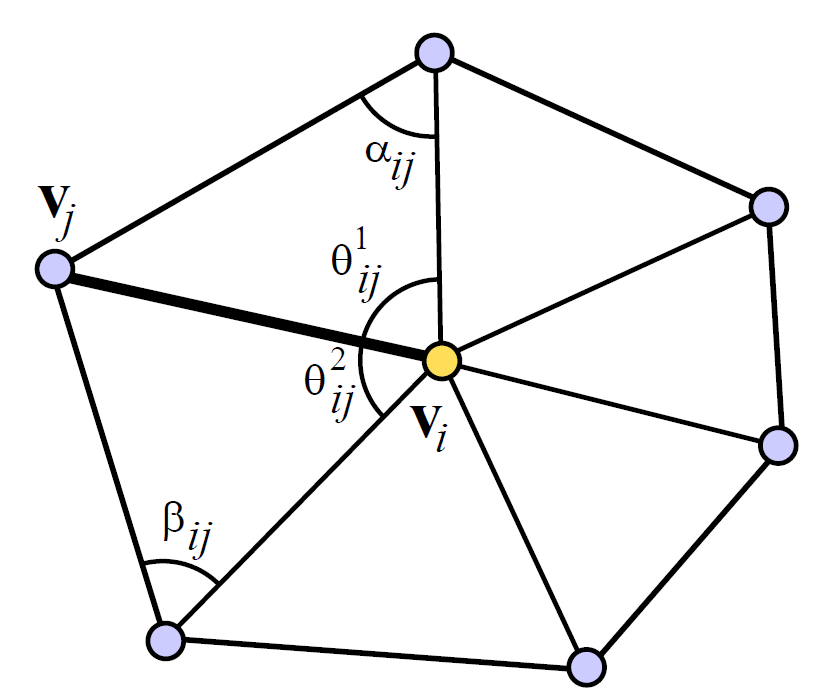
\includegraphics[width=0.5\linewidth]{cot_weight}
  \caption[Angles in cotangent weights]{Angles in cotangent weights (courtesy of \cite{Sorkine:EG:2005}).}
\label{fig:cotweights}
\end{figure}

To faithfully approximate smooth Laplacian on arbitrary meshes, we need to take
into account geometric information such as the distances between neighboring
vertices and the angles between contiguous edges. Such defined Laplacian is
called the \emph{geometric Laplacian}.

Constructing discrete Laplace-Beltrami operator on general meshes is not a trivial task.
In fact, it is impossible to make discrete Laplacian to simultaneously converge to smooth
Laplacian and be symmetric on general meshes~\cite{Rustamov:2007:LEF}. Many different
versions of geometric discrete Laplacian have been proposed
~\cite{pinkall1993computing, Desbrun1999, Xu:2004:GMP, Levy2006, Vallet2008, Belkin:2008:SCG}.
One of the most popular scheme was proposed by Meyer et al.~\cite{Meyer2003}.
It uses the cotangents of the two angles opposite to an edge to weight the edge,
and the area of the Voronoi cell size surrounding a vertex to weight the vertex.
Its action on vertex-based function $f$ on mesh $M$ is

\begin{equation}
\Delta f(v_i)=\frac{1}{a_i}\sum_{j\in N(i)}w_{ij}\frac{f(v_i)-f(v_j)}{d_i}.
\end{equation}

Here $a_i$ is the area of the Voronoi cells around vertex $v_i$, and the weights

\begin{equation}
w_{ij}:=\frac{\cot\alpha_{ij}+\cot\beta_{ij}}{2},
\end{equation}

where $\alpha_{ij}$ and $\beta_{ij}$ denote the two angles opposite to the edge $(v_i,v_j)$
(See Fig.~\ref{fig:cotweights}).

Let us define the area matrix $A=diag(a_i)$ and weight matrix $W$ as
\begin{equation*}
W(i,j)=\left\{
       \begin{array}{lc}
        \sum_{k\in N(i)}w_{ik}\quad & i=j \\
        -w_{ij}\quad & (v_i,v_j)\in E \\
        0\quad & \text{otherwise}
    \end{array}
\right.
\end{equation*}
The geometric Laplacian matrix then can be written as $L=A^{-1}W$.

Generally, such defined $L$ is not symmetric. However, we can rewrite the the
equation $L\mathbf{\phi}=\lambda\mathbf{\phi}$ as the generalized eigenvalue
problem

\begin{equation}
\label{eq:geneigen}
W\mathbf{\phi}=\lambda A\mathbf{\phi}.
\end{equation}

Since $W$ is symmetric and $A$ is symmetric positive-definite, the generalized
eigenvectors $\mathbf{\phi_i}$ corresponding to different generalized eigenvalues
$\lambda_i$ are orthogonal, and all of the generalized eigenvalues/eigenvectors
are real. We should note that the orthogonality is with respect to the inner product
induced by $A$

\begin{equation}
\langle\mathbf{\phi_i},\mathbf{\phi_j}\rangle=\mathbf{\phi_i}^T A \mathbf{\phi_j}=0,\quad i\neq j.
\end{equation}

If the mesh vertices are evenly distributed, i.e., each vertex has the same Voronoi
cell size, we can make $A=I$ by proper normalization. In this case, the $A$-inner
product becomes the standard dot product ($I$-inner product). This is unfortunately
not valid for general meshes whose vertices are not distributed uniformly over the
surface area. We may adopt the symmetric version of mesh Laplacian $L_s = A^{-1/2}WA^{-1/2}$,
which will give the same eigenvalues~\cite{Vallet2008}. The original eigenvectors can be
obtained by $\mathbf{\phi_i}=W^{-1/2}\mathbf{\phi^s_i}$. However, this symmetrization is not
preferable since solving the generalized eigenvalue problem is more stable than
inverting $W$~\cite{Reuter:CG:2009}.

Let $\{\lambda_i\}_{i=0}^{N-1}$ be the set of generalized eigenvalues of
$\Delta_M=A^{-1}W$, and $\{\mathbf{\phi_i}\in\mathbb{R}^N\}$ their corresponding
eigenvectors. A square-integrable scalar function $\mathbf{f}$ defined on $V$ can
be expanded as the linear combination of the eigenvectors

\begin{equation}
\mathbf{f}(p)=\sum_{k=0}^{N-1}\langle \mathbf{f},\mathbf{\phi_k}\rangle_A \mathbf{\phi_k}(p),
\end{equation}

where the inner-product is the $A$-induced scalar product

\begin{equation}
\langle \mathbf{f},\mathbf{g}\rangle_A = \mathbf{f}^T A\mathbf{g}=\sum_{i=0}^{N-1}a_i \mathbf{f}(i)\mathbf{g}(i).
\end{equation}

Unlike classic Fourier basis functions which are simply fixed sinusoids, the
manifold harmonic basis differ with the connectivity, geometry, and the type
of Laplacian operator that is adopted~\cite{Zhang:2010:CGF}. As a result, the
mesh Laplacian eigenvectors and eigenvalues actually encode substantial topological
and geometric information and can help characterize the global shape property and
reveal intrinsic structure of the original mesh. In addition, Laplace-Beltrami
operator is globally defined and is completely determined by the metric tensor,
which is itself an isometry invariant. Hence, the Laplacian eigenvalues and eigenfunctions
encode meaningful global intrinsic information about the shape and they are invariant
under isometric deformations up to a change in sign~\cite{Rustamov:2007:LEF,Sun:2009:CGF}.
This lends to the popularity of spectral methods in the area of geometry processing
and analysis.

Directly employing the eigenstructures of mesh Laplacian, a great diversity of spectral
methods have been developed for shape modeling problems including compression~\cite{Karni2000},
segmentation~\cite{Liu2007}, deformation~\cite{Rong2008}, remeshing~\cite{dong2006spectral},
paramterization~\cite{Zhou2004}, shape indexing~\cite{Reuter:2006:CAD, Rustamov:2007:LEF},
and retrieval~\cite{Lavoue:2012}. We refer readers to \cite{Zhang:2010:CGF} for a more thorough
review of the theories and applications of mesh Laplacian spectra.

\section{Kernels and Spectral Graph Wavelets}

\subsection{Kernel Functions}

The concept of manifold/graph Fourier transform can be extended to the 
bivariate case to define kernels. Suppose we have a bivariate kernel
$\theta:\mathcal{M}\times\mathcal{M}\to\mathbb{R}$ which corresponds to a
self-adjoint operator $\Theta$. The bivariate kernel $\theta$ can be expanded
on the manifold Fourier basis

\begin{equation}
\theta(x,y)=\sum_{k=0}^\infty \hat{\theta}(k)\phi_k(x)\phi_k(y),
\end{equation}

where

\begin{equation}
\hat{\theta}(k)=\langle\langle\theta(x,y),\phi_k(x)\rangle,\phi_k(y)\rangle.
\end{equation}

$\hat{\theta}(k)$ can be deemed as the Fourier transform of the bivariate kernel
with a slight abuse of language.

For example, the Laplace-Beltrami operator itself can be expanded as
\begin{equation}
\Delta_\mathcal{M}(x,y)=\sum_{i=0}^\infty \lambda_k\phi_k(x)\phi_k(y).
\end{equation}

Hence, its Fourier transform is $\widehat{\Delta_\mathcal{M}}(k)=\lambda_k$.

The kernel function $\theta(x,y)$ describes the relations between each pair of
points on the manifold, and its diagonal $\theta(x,x)$ affords a
signature function for the characterization of individual points.

One well known kernel function is the heat kernel $K(t,x,y)$, which is
the fundamental solution to the heat equation with appropriate boundary condition. 
For example, the heat kernel for the Dirichlet problem is solution to the equation

\begin{equation}
\left\{
  \begin{array}{ll}
    \frac{\partial K}{\partial t}(t,x,y) = \Delta_{\mathcal{M}} K(t,x,y) &\forall t>0 ~\text{and}~ \forall x,y\in\mathcal{M}\\
    \lim_{t\rightarrow 0}K(t,x,y)=\delta_x(y) &\forall x,y\in\mathcal{M} \\
    K(t,x,y)=0. & x\in\partial\mathcal{M} ~\text{or}~ y\in\partial\mathcal{M}
  \end{array}
\right.
\end{equation}

Expanded on the manifold harmonic functions, the heat kernel with time parameter
$t$ has the following expression:

\begin{equation}
K(t,x,y)=\sum_{k=0}^{\infty} e^(-\lambda_k t) \phi_k(x)\phi_k(y).
\end{equation}

On the mesh domain, the heat kernel affords a multi-scale, stable and intrinsic
characterization of the geometric shape~\cite{Sun:2009:CGF}, and have been
the foundation for many shape analysis applications including shape matching~\cite{Ovsjanikov2010}
and shape retrieval~\cite{Bronstein2011}.


\subsection{Wavelets on Graphs}

Wavelet is a powerful analytical tool in signal processing. Intuitively speaking,
a wavelet is just a wave-like pulse in time (or space). By scaling and translating
a single mother wavelet, we may obtain a family of wavelet functions that cover
the entire domain in question. Similar to Fourier analysis in which a function $f$
can be decomposed into a series of component harmonics, in wavelet analysis $f$
can be expanded by a family of component wavelets. Nevertheless, there are some
fundamental differences between the Fourier and wavelet analysis:

\begin{itemize}
\item In Fourier analysis, each component harmonic is globally defined in space/time. In wavelet analysis, the component wavelet are all locally defined at different locations.
\item In Fourier analysis, each component harmonic has an exclusive frequency. In wavelet analysis, we use multiple wavelets localized at different locations to represent the information of a single frequency. Generally, for large scale information (low frequency), we use fewer wavelets; whereas for small scale information (high frequency), we use more wavelets.
\item The component harmonics in Fourier analysis are all orthogonal to each other. In fact, the Fourier basis functions form an orthonormal basis of the space of square-integrable functions. This is not necessarily true for wavelet functions.
\end{itemize}

In a nutshell, wavelet functions can be simultaneously localized in both time/space and frequency domain,
in contrast to the Fourier transform in which the basis harmonic functions are all globally defined
in time/space. For signals whose primary information lies in localized singularities, such as edges
in images or step discontinuities in time series signals, wavelet transform affords a more compact
representations than a transform with global basis such as the Fourier transform.

There have been many efforts to introduce wavelet methods to the field of visual computing.
Representative applications include image segmentation \cite{Figueiredo:2005:CVPR},
image-based rendering \cite{Overbeck:2009:TOG}, volume rendering \cite{Lippert:1995},
scientific visualization \cite{Cracium:2005:TVCG}, spectral rendering \cite{Iehl:2000:CGF},
animation compression \cite{Payan:2007:CG}, etc.

Classical wavelets are constructed by translating and scaling a mother wavelet in Euclidean
space, however, transplanting wavelets to graphs (specifically, triangular meshes) is not
straightforward due in part to the fact that it is unclear how to apply the scaling operation
on a signal that is defined on the mesh vertices, so early studies using wavelet mostly
relied on the spherical parameterization~\cite{Werghi:2002,Liu:2007}.

One popular scheme to imitate scaling on meshed surfaces is achieved via explicit subdivision,
which iteratively refines the mesh geometry, and at the same time, also refines the functions
defined on the mesh. The constructed wavelets are biorthogonal and locally supported.
The subdivision wavelets rely on the subdivision connectivity of the mesh, which restricts the
application scope to data compression and level-of-detail rendering. The idea of subdivision
wavelets was first proposed by Schr\"{o}der and Sweldens \cite{Schroder:1995:SIGGRAPH}, in
which the lifting scheme was used to construct wavelets on sphere.
Lounsbery et al. \cite{Lounsbery:1997:TOG} studied MRA of wavelets constructed on surfaces
of arbitrary topology type. In \cite{Bertram:2000:vis}, Bertram et al. utilized bicubic
B-spline subdivision to construct wavelet transform that affords boundary curves and sharp
features. As a drawback, the subdivision wavelet
requires the meshes to have subdivision connectivity, where remeshing process is frequently
needed. To avoid remeshing, Valette and Prost \cite{Valette:2004:TVCG} extended the subdivision
wavelet for triangular meshes using irregular subdivision scheme that can be directly computed
on irregular meshes. On spherical domains, Haar wavelets \cite{Nielson:1997:vis,Bonneau:1999:vis}
were constructed over nested triangular grids generated by subdivision. Recently, the spherical
Haar wavelet basis was improved to the SOHO wavelet basis \cite{Lessig:2008:TOG} that is both
orthogonal and symmetric.

Another method to construct graph and mainfold wavelets is
through diffusion~\cite{Coifman2006, Hou2013}.
In sharp contrast to the aforementioned subdivision wavelets, the diffusion
wavelets adopt a bottom-up philosophy starting from the fine input data.
The \emph{Diffusion wavelets} ~\cite{Coifman2006} use a diffusion operator
and its powers to expand the nested subspaces, where scaling functions and
wavelet functions are obtained by orthogonalization and rank-revealing
compression. This diffusion-driven methodology naturally dilates the
functions associated with the underlying heat diffusion process, which solely
depends on manifold geometry. It allows flexible construction directly from data.
However, the constructed scaling and wavelet functions are not locally-supported,
which limits the functionality of space localization. In fact, it is impossible
to construct wavelets that are simultaneously fully orthogonal, locally supported,
and symmetric \cite{Lounsbery:1997:TOG}. As an improvement, the biorthogonal
diffusion wavelets (BDW) \cite{Maggioni:2005:SPIE} were introduced, relieving the
excessively-strict orthogonality property of scaling functions.
In \cite{Mahadevan2005}, diffusion wavelets were adopted to approximate
scalar-valued functions based on analyzing the structure and topology of the
state space. Rustamov \cite{Rustamov:2009:ICMS} studies the relation between
mesh editing and diffusion wavelets by introducing the generalized linear
editing (GLE). However, neither the DW nor the BDW have achieved localization
in both manifold and frequency domain.

In \cite{Hou2013}, an admissible diffusion wavelets (ADW) on meshed surfaces and point clouds is proposed.
The ADW are constructed in a bottom-up manner that starts from a local operator in a high frequency,
and dilates by its dyadic powers to low frequencies. By relieving the orthogonality and enforcing normalization,
the wavelets are locally-supported and admissible.

It is attractive to be able to define wavelet transform directly on 3D
shapes without the need of parameterization. Various schemes of
manifold wavelets have been proposed via different
approaches~\cite{Antoine2010189}. Diffusion wavelets, introduced by
Maggioni and Coifman~\cite{Coifman2006}, use diffusion as a
scaling tool to achieve multiscale analysis. Wavelet and scaling
functions are constructed by repeatedly applying a diffusion operator
$T$ on the graph or manifold space. After applying dyadic powers of
$T$ at each scale, a localized orthogonalization procedure is
performed to yield nested approximation spaces, and then wavelets are
produced by locally orthogonalizing vectors spanning the difference of
these approximation spaces. The derived diffusion wavelets are
orthogonal, compact, and multiscale in nature, and have been employed
in 3D mesh compression
in~\cite{mahadevan2007AdaMesCom3DComGraUsiMulManLea}.
In~\cite{gavish2010multiscale,ram2012redundant}, tree-based,
data-adaptive wavelet transforms are developed for high-dimensional
Euclidean data sets and weighted graphs, under the assumption that the
data have a rich geometrical structure that can be captured by a
hierarchical tree.

\subsection{Spectral Graph Wavelets}

The primary reason that classical wavelet transforms cannot be directly adapted to graph or manifold is
that for a mother function $\psi(x)$ defined on a manifold,
there is no obvious definition for $\psi(sx)$. One approach to solve this problem is appealing to the Fourier domain,
with the help of aforementioned manifold harmonics. Although scaling cannot be explicitly expressed on manifold domain,
it can be easily defined on the frequency domain. The idea of spectral wavelet transform was introduced in \cite{Hammond2011}
on the graph domain, denoted as the Spectral Graph Wavelet Transform (SGWT). Here we extend the concept to general manifold,
denoted as the Spectral Graph Wavelet Transform (SGWT)

Given manifold $\mathcal{M}$ with appropriate boundary condition. Assume its Laplace-Beltrami operator $\Delta_\mathcal{M}$ has the eigen-decomposition $\{\lambda_k,\phi_k\}$. The eigenvectors $\{\phi_k\}$ form a complete and orthonormal basis of $L^2(\mathcal{M})$, commonly known as the manifold harmonics. The corresponding eigenvalues $\{\lambda_k\}$ satisfy
\begin{equation}
0=\lambda_0 < \lambda_1 \leq \lambda_2 \leq \cdots
\end{equation}

For any function $f$ defined on $\mathcal{M}$, its generalized Fourier transform $\hat{f}$ is defined as
\begin{equation}
\hat{f}(k)=\langle \phi_k, f \rangle=\sum_{k=0}^\infty \phi_k(x)f(x)
\end{equation}

And the inverse Fourier transform is
\begin{equation}
f(x)=\sum_{k=0}^\infty\hat{f}(k)\phi_k(x)
\end{equation}

The Parseval relations holds for the manifold harmonics transform
\begin{equation}
\label{eq:parseval}
\langle f,g\rangle=\langle\hat{f},\hat{g}\rangle
\end{equation}

\begin{figure}[!to]
\begin{center}
\includegraphics[width=\linewidth]{4_SGW}
\end{center}
\caption[Spectral graph wavelets on the wolf model.]{Spectral Graph Wavelets centered at one vertex on the wolf model.
  From left to right are wavelets from high frequency to low frequency with
  scale 1, 3 and 5.}
\label{SGW}
\end{figure}

We generate SGWT from a special wavelet operator that acts on functions defined on the manifold. Given a real-valued transfer function $g$, the wavelet operator $T_g$ is defined by how it modulate on $f:\mathcal{M}\to\mathbb{R}$ on Fourier domain
\begin{equation}
\widehat{T_g f}(k)=g(\lambda_k)\hat{f}(k)
\end{equation}

Employing the inverse Fourier transform, we obtain the spectral representation of $T_g f$
\begin{equation}
\label{eq:waveletop}
(T_g f)(\cdot)=\sum_{k=0}^\infty g(\lambda_k)\hat{f}(k)\phi_k(\cdot)
\end{equation}

To obtain spectral wavelets, we need localized and scaled versions of $T_g f$. The scaling is defined by dilating the transfer function as $g(t\lambda_k)$. The localization at point $x\in\mathcal{M}$ is realized by applying wavelet operators to unit impulse at $x$, represented by the Dirac delta function $\delta_x(\cdot)$

Since
\begin{equation}
\delta_x(\cdot)=\sum_{k=0}^\infty\phi_k(x)\phi_k(\cdot)
\end{equation}
We have the Fourier transform of $\delta_x$
\begin{equation}
\hat{\delta_x}(k)=\phi_k(x)
\end{equation}

Set $f=\delta_x$ in (\ref{eq:waveletop}), we have the spectral wavelet at scale $t$ and localized at point $x$
\begin{equation}
\psi_{t,x}(\cdot)=(T^t_g\delta_x)(\cdot)=\sum_{k=0}^\infty g(t\lambda_k)\phi_k(x)\phi_k(\cdot)
\end{equation}

The spectral wavelet can also be represented as a bivariate kernel
\begin{equation}
\Psi_t(x,y)=\psi_{t,x}(y)=\sum_{k=0}^\infty g(t\lambda_k)\phi_k(x)\phi_k(y)
\end{equation}

For a real-valued function $f$ defined on $\mathcal{M}$, the spectral wavelet transform is
\begin{equation}
\mathcal{W}^\psi_f(x,t)=\langle\psi_{x,t},f\rangle
\end{equation}

Applying the Parseval relation (\ref{eq:parseval}), we obtain the spectral representation of continuous spectral wavelet transform
\begin{equation}
\mathcal{W}^\psi_f(x,t)=\langle\hat{\psi_{x,t}},\hat{f}\rangle=\sum_{k=0}^\infty\hat{\psi_{x,t}}(k)\hat{f}(k)=\sum_{k=0}^\infty g(t\lambda_k)\hat{f}(k)\phi_k(x)
\end{equation}

If seen as a function of $x$, the Fourier transform of the above spectral wavelet transform is
\begin{equation}
\widehat{\mathcal{W}^\psi_f}(k)=g(t\lambda_k)\hat{f}(k)
\end{equation}

Similar to classical wavelet transform, the spectral wavelet transform is invertible only if the transfer function $g$ satisfies the admissibility condition
\begin{equation}
C_\psi=\int_0^\infty\frac{g^2(a)}{a}da<\infty
\end{equation}
and the zero-mean condition $g(0)=0$.

%Then we consider the summation of wavelets $\psi_{t,x}$ multiplied by corresponding wavelet coefficient $\mathcal{W}^\psi_f(t,x)$, subject to a non-constant weight $dt/t$
%\begin{align*}
%  & \sum_{x\in\mathcal{M}}\int_0^\infty\frac{\mathcal{W}^\psi_f(x,t)\psi_{x,t}(y)}{t}dt \\
%= & \int_0^\infty\frac{dt}{t}\sum_{x\in\mathcal{M}}\mathcal{W}^\psi_f(x,t)\psi_{y,t}(x) \\
%= & \int_0^\infty\frac{dt}{t}\sum_{k=0}^\infty\hat{\mathcal{W}}^\psi_f(k)\hat{\psi}_{y,t}(k) \\
%= & \int_0^\infty\frac{dt}{t}\sum_{k=0}^\infty(g(\lambda_k t)\hat{f}(k))(g(\lambda_k t)\phi_k(y)) \\
%= & \sum_{k=0}^\infty(\int_0^\infty\frac{|g(\lambda_k t)|^2 dt}{t})\hat{f}(k)\phi_k(y) \\
%= & (\int_0^\infty\frac{|g(a)|^2da}{a})\sum_{k=1}^\infty\hat{f}(k)\phi_k(y) \\
%= & C_\psi(f(y)-\hat{f}(0)\phi_0(y))
%\end{align*}

%This yields the formula of inverse continuous spectral wavelet transform
%\begin{equation}
%f(y)=\frac{1}{C_\psi}\int_0^\infty\frac{\mathcal{W}_f^\psi(x,t)\psi_{x,t}(y)}{t}dt+\hat{f}(0)\phi_0(y)
%\end{equation}

\begin{figure}
  \centering
  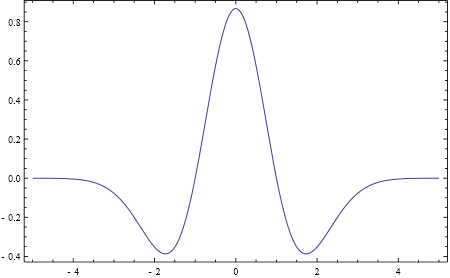
\includegraphics[width=0.5\linewidth]{1DMexicanHat}\\
  \caption{1D Mexican-hat Wavelet}
  \label{fg:1DMexicanHat}
\end{figure}

\begin{figure}
  \centering
  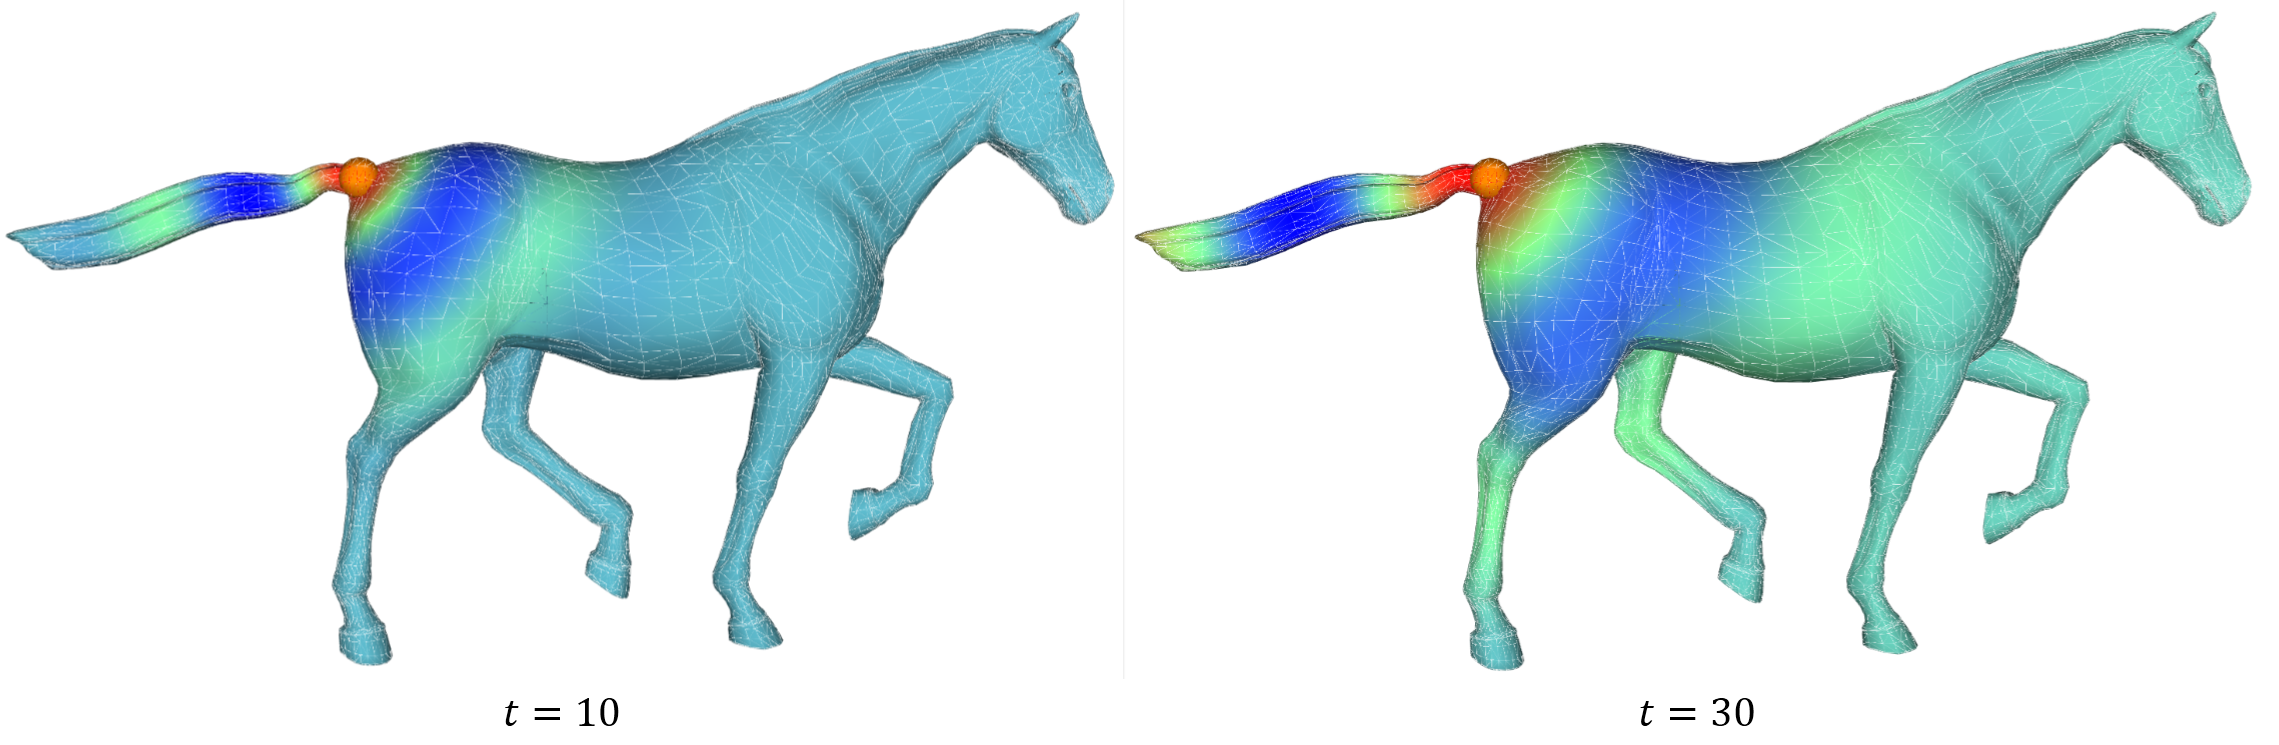
\includegraphics[width=\linewidth]{MexicanHatWavelet}\\
  \caption[Color plots of the spectral Mexican-hat wavelets.]
  {Color plots of the spectral Mexican-hat wavelet with scales of 10 and 30. The reference point is denoted by the orange ball. We can easily spot the function values oscillate around the reference point. When t is larger, the period of oscillation also increases.}
  \label{fg:MexicanHatWavelet}
\end{figure}

\begin{figure}
  \centering
  \includegraphics[width=0.8\linewidth]{WaveletFrequency}\\
  \caption[Transfer function of the Mexican-hat wavelet.]
  {The Mexican-hat wavelet transfer function in the frequency domain. }\label{fg:WaveletFrequency}
\end{figure}

In classical wavelets defined on real line, the space localization is apparent. If the mother wavelet $\psi(x)$ is localized in the interval $[-\epsilon,\epsilon]$, then the wavelet $\psi_{a,b}(x)$ will be localized with $[b-a\epsilon,b+a\epsilon]$. in the limit as $b\to 0$, $\psi_{a,b}(x)\to 0$ for $x\neq b$.

For spectral wavelets, the localization property is less straightforward since the scaling is defined implicitly in the Fourier domain. For $g$ sufficiently regular, the normalized spectral wavelet $\psi_{t,x}/\|\psi_{t,x}\|$ will vanish on vertices sufficiently far from $x$ in the limit of fine scales, i.e. as $t\to 0$. We should expect $\psi_{t,x}(y)$ to be small if $x$ and $y$ are separated and $t$ is small.

If two transfer functions $g$ and $g'$ are close to each other, then the derived spectral wavelets should be close to each other in the manifold domain.

As an example, we consider the Mexican hat wavelet. In 1D Euclidean space, the Mexican hat wavelet is defined as
\begin{equation}
\psi(t)=\frac{2}{\sqrt{3\sigma}\pi^{\frac{1}{4}}}(1-\frac{t^2}{\sigma^2})e^{\frac{-t^2}{2\sigma^2}}.
\end{equation}
Its graph is shown in Fig.~\ref{fg:1DMexicanHat}, which exhibits clear localization in space. In manifold space, we may analogously define the spectral Mexican hat wavelet as
\begin{equation}
\psi_{t,x}(\cdot)=\sum_{k=0}^\infty t^2\lambda_k^2 e^{-t^2\lambda_k^2}\phi_k(x)\phi_k(\cdot),
\end{equation}
with the transfer function $g(t\lambda)=t^2\lambda^2 e^{-t^2\lambda^2}$.

Fig.~\ref{fg:MexicanHatWavelet} visualizes the value of the wavelet functions over the surface, with the scale $t=10$ and $t=30$. Fig.~\ref{fg:WaveletFrequency} shows the Fourier transform of the wavelet functions in frequency domain. It is easy to see that

\begin{itemize}
\item The spectral wavelet function is localized both in manifold and frequency domain.
\item On manifold, the values of the spectral wavelet functions attenuate and oscillate as the distance from the reference point increases.
\item For a larger scale, the Mexican hat wavelet has a wider windows in space, but a narrower window in frequency.
\end{itemize}

By construction, the spectral wavelets $\psi_{t,x}$ are all orthogonal to the the null eigenvector $\phi_0$,
and nearly orthogonal to $\phi_l$ for $\lambda_l$ near zero \cite{Hammond2011}.

Spectral scaling functions are determined by a single real valued function $h:\mathbb{R}^+\to\mathbb{R}$,
which acts as a low-pass filter and satisfies $h(0)>0$ and $\lim_{x\to\infty}h(x)\to 0$.
Introducing the scaling functions helps ensure stable recovery of the original signal $f$ from the wavelet
coefficients when the scale parameter $t$ is sampled at discrete values ${t_j}$.
Stable recovery will be assured if $G(\lambda)=h(\lambda)^2+\sum_{j=1}^J g(t_j\lambda)^2$ is
bounded away from zero. The design of the scaling function generator $h$ is uncoupled from the choice $g$.

The spectral wavelets depend on the continuous scale parameter $t$. For practical computation,
$t$ must be sampled at a finite number of scales $\{t_j\}_{j=1}^J$, which generates
$NJ$ wavelets $\psi_{t_j,n}$ along with $N$ scaling functions $s_n$. It can be proven~\cite{Hammond2011}
that the set $\Gamma=\{\phi_n,n=0,\ldots,N-1\}\cup\{\psi_{t_j,n},j=1,\ldots,J,n=1,\ldots,N\}$
form a frame with bounds
\begin{equation*}
A=\min_{\lambda\in[0,\lambda_{N-1}]}G(\lambda)
\end{equation*}
and
\begin{equation*}
B=\max_{\lambda\in[0,\lambda_{N-1}]}G(\lambda),
\end{equation*}
where $G(\lambda)=h^2(\lambda)+\sum_j g(t_j\lambda)^2$. That is to say, for all $f$ defined on the manifold, the following inequality holds
\begin{equation}
A\|f\|^2\leq\sum_k|\langle f,\Gamma_k\rangle|^2\leq B\|f\|^2,
\end{equation}
where $\Gamma=\{\Gamma_k\}$.

The spectral wavelet transform is an overcomplete transform, mapping
an input vector $f$ of size $N$ to $N(J+1)$ coefficients $c=Wf$.
Given a set of coefficients $c$, the synthesis/reconstruction of $f$ can be given by solving the matrix equation
\begin{equation}
(W^*W)f=W^*c.
\end{equation}

Because of its attractive and powerful properties such as spatial localization,
multiscale, and geometry awareness, SGW has already been adopted as a descriptor
for a handful of shape analysis applications. Kim et al.~\cite{Kim:2012,Kim:2014}
introduced a wavelet-based multi-scale descriptor for the analysis of
cortical surface signals using the SGWT and Li et al.~\cite{Li:2013}
proposed a SGWT-based descriptor and utilized the intrinsic spatial
pyramid matching (ISPM) for global shape retrieval. Though these
researches discover the potentials of SGWs, they all concentrate on
global shape analysis based on point signatures, ignoring the SGWs'
power in integrating the local-to-global geometrical and topological information.

\section{Sparse Representation Modeling}

In recent years, sparse modeling techniques have become
increasingly popular in various fields of signal processing and
analysis, especially in image processing and computer vision. Its
widespread applications include data compression, signal denoising,
pattern recognition, etc.

The fundamental idea of sparse modeling is to decompose or approximate the
signal in question as the linear combination of a very small subset of vectors
selected from a large number of candidate elementary vectors. These candidate
elementary vectors, also called \emph{atoms}, constitute a set called the
\emph{dictionary}. With a given dictionary, the signal is encoded by the
coefficients w.r.t. the selected atoms and can be easily reconstructed. The
rationale of sparse modeling is that most meaningful high-dimensional signals probably
have some intrinsic structures or patterns, which can be exploited for
efficient representation in a subspace of much lower dimension. Because of
the versatility of the input signals, it is often desirable for dictionaries to
be redundant or overcomplete, allowing greater freedom and flexibility in
design to accommodate a sparse set of atoms that can better capture
an input signal's intrinsic characteristics.

\subsection{Sparse Modeling Problems}

Consider signal $\mathbf{b}\in\mathbb{R}^n$ and dictionary matrix
$\mathbf{D}\in\mathbb{R}^{n\times m}$ with $n<m$. If the dictionary constitutes an
overcomplete basis of $\mathbb{R}^n$, the linear systems of
equations $A\mathbf{x}=\mathbf{b}$ is underdetermined and has infinite solutions.

To make the solution $\mathbf{x}$ unique, we could introduce an objective function
$J(\mathbf{x})$ to govern the desired properties of the solution vector $\mathbf{x}$.
The general optimization problem subject to linear equality constraints is as follows:

\begin{equation}
\label{eq:constrained-inverse}
\min_\mathbf{x} J(\mathbf{x}) \quad \mathrm{subject\,to} \quad \mathbf{b}=\mathbf{D}\mathbf{x}.
\end{equation}

Alternatively, the objective function can be used as a regularization term, giving rise to
the following regularized least square problem:

\begin{equation}
\label{eq:regularized-ls}
\min_\mathbf{x} \|\mathbf{b}-\mathbf{D}\mathbf{x}\|_2^2 + \lambda J(\mathbf{x}).
\end{equation}

The regularization term can be viewed as imposing certain priors distributions on
the solution $\mathbf{x}$. Comparing with Eq.~\ref{eq:constrained-inverse}, regularization
allows users to control the tradeoff between the reconstruction fidelity and the
desired property (e.g., smoothness) of the solution and avoids overfitting.

Eq.~\ref{eq:constrained-inverse} and Eq.~\ref{eq:regularized-ls} are commonly encountered in different
areas, including signal processing, machine learning, and statistics. One common choice for $J(\mathbf{x})$
is the function of squared $l_2$-norm $\|\mathbf{x}\|_2^2$, which aims to minimize the ``energy'', or Euclidean
norm of the solution vector. Eq.~\ref{eq:constrained-inverse} then has the closed-form

\begin{equation}
\hat{\mathbf{x}}=\mathbf{D}^T(\mathbf{D}\mathbf{D}^T)^{-1}\mathbf{b}=\mathbf{D}^{+}\mathbf{b},
\end{equation}
where $\mathbf{D}^{+}=\mathbf{D}^T(\mathbf{D}\mathbf{D}^T)^{-1}$ is the pseudo-inverse
of $\mathbf{D}$. Let $J(\mathbf{x})=\mathbf{\Gamma}\mathbf{x}$, where $\mathbf{\Gamma}\in\mathbb{R}^{m\times m}$,
Eq.~\ref{eq:regularized-ls} then becomes the famous Tikhonov regularization~\cite{Golub1999}, which has the
explicit solution
\begin{equation}
\hat{\mathbf{x}} = (\mathbf{D}\mathbf{D}^T + \lambda \mathbf{\Gamma}\mathbf{\Gamma}^T)^{+}\mathbf{D}^T\mathbf{b}.
\end{equation}

Due to its computational simplicity, the $l_2$ norm is commonly used as the or penalty term. However, for
many applications, minimizing the total energy of solutions is not very meaningful.

If we know that the signal $\mathbf{b}$ has a very sparse coefficient representation $\mathbf{x'}$ with respect
to $\mathbf{D}$, i.e., $ \mathbf{b} \approx \mathbf{D}\mathbf{x'}, \|\mathbf{x'}\|_0 \ll m$,
then we can specify $J(\mathbf{x})$ such that the objective to minimize the number of non-zero coefficients
in solution $\mathbf{x}$. The resultant optimization problem is called sparse decomposition and can be
formulated as follows:

\begin{equation}
\label{eq:sparse-decompose}
\min_\mathbf{x} \|\mathbf{x}\|_0 \quad \mathrm{subject\,to} \quad \mathbf{b}=\mathbf{D}\mathbf{x}.
\end{equation}

Here $\|\mathbf{x}\|_0$ denotes the pseudo norm of $\mathbf{x}$ which counts the number
of non-zero elements in $\mathbf{x}$.

For real life signals, exact sparsity w.r.t. a fixed dictionary is elusive; instead, natural
signals tend to be \emph{compressible}, meaning that the representation coefficients decay rapidly
when sorted in order of decreasing magnitude. Hence, a more practical formulation is to allow a bounded
error of the sparsely reconstructed signal $\mathbf{D}\mathbf{x}$, giving rise to the best
subset selection problem:
\begin{equation}
\label{eq:sparse-approx}
\min_\mathbf{x} \|\mathbf{x}\|_0 \quad \mathrm{subject\,to} \quad \|\mathbf{b}-\mathbf{D}\mathbf{x}\|_2^2<\epsilon.
\end{equation}
or written as a regularization problem,
\begin{equation}
\label{eq:regularized-sparse-approx}
\min_\mathbf{x}  \|\mathbf{b}-\mathbf{D}\mathbf{x}\|_2^2 + \lambda \|\mathbf{x}\|_0
\end{equation}

Clearly, the approximation quality and the sparsity of the coefficient vector depend both on the signal itself
and the dictionary $\mathbf{D}$. We can expect more concise and accurate coefficient representations if the atoms
in $\mathbf{D}$ can better capture properties of concerned signal. Take the 2D image domain as example. The global
Fourier basis vectors are suitable for representing global signal trends, while wavelets, with its local support,
can better represent isotropic features of different scales. To efficiently encode anisotropic image feature
such as lines and curves, various extensions to wavelets have been proposed
including contourlet~\cite{Do2005}, ridgelets~\cite{Emmanuel1999}, curvelets~\cite{Candes1999}, etc. By incorporating
new design parameters such as directions, these new shape basis afford more effective characterization of images
dominated with different features.

\subsection{Computational Methods}
The $l_0$ optimization problems (Eq.~\ref{eq:sparse-decompose} and Eq.~\ref{eq:sparse-approx}) are NP-hard,
so searching through all possible support sets by brute force is intractable except for problems of very small
sizes. A variety of methods have been developed for finding near-optimal solution to $l_0$ optimization, and
the most important two classes are \emph{greedy pursuit} and \emph{convex relaxation}~\cite{Tropp2010}.

\subsubsection*{Greedy Pursuit Methods}
One of the most commonly-used approaches to sparse approximation is
the greedy pursuit method. The central idea is to iteratively refine a
sparse solution in a greedy manner. More specifically, in each
iteration one or more atoms of the dictionary are chosen
and the corresponding coefficients are modified
such that the greatest improvement in approximation quality can be achieved.
Representative greedy pursuit algorithms include matching pursuit
(MP)~\cite{Mallat1993}, orthogonal matching pursuit
(OMP)~\cite{Pati1993}, and simultaneous orthogonal matching pursuit (S-OMP)~\cite{Tropp2006a}.
The latter is suitable for solving the simultaneous sparse approximation problem where
the input signal have multiple correlated channels and the same subset of atoms is to be used
for every channel.


The basic idea of greedy pursuit methods is to iterative refine the estimation of the coefficient vector
$\mathbf{x}$. In each step, one or several coefficients are modified to yield biggest possible improvement
in approximating the signal. The simplest greedy pursuit algorithm is \emph{matching pursuit (MP)}~\cite{Mallat1993},
described as follows
\begin{enumerate}
\item Set the index set $\Omega=\emptyset$, the residual $\mathbf{r_0} = \mathbf{b}$, and the counter $k=1$.
\item Find an index $n_k$ such that atom $\mathbf{\alpha}_{n_k}$ is most correlated with the residual
\begin{equation*}
n_k = \argmax_n |\langle \mathbf{r}_{k-1},\mathbf{\alpha}_{n} \rangle|,
\end{equation*}
and add $n_k$ to $\Omega$. The coefficient corresponding to $\mathbf{\alpha}_{n_k}$ is denoted as $x_{n_k}$.

\item Update the residual $\mathbf{r}_k = \mathbf{r}_{k-1} - x_{n_k} \mathbf{\alpha}_{n_k}$.
\item Increment $k$. Repeat (2)-(4) until stopping criterion is met.
\end{enumerate}

The possible stopping criteria can be that a fixed number of atoms have been selected, the magnitude of residual is
smaller than a threshold, or no remaining atoms have strong correlation with the residual.

A much improved version of MP is the algorithm known as \emph{orthogonal matching pursuit (OMP)}~\cite{Pati1993}.
The major difference with MP is an additional step of coefficients update. After a new index (that is most strongly
correlated with the residual) is identified and added to the index set $\Omega$,
the coefficients calculated in previous steps are replaced with new coefficients which approximate the original signal
in the least square sense. Contemporary greedy pursuit methods have more sophisticated mechanism for selecting and
pruning the set of active atoms, including the stagewise orthogonal matching pursuit (StOMP)
~\cite{Donoho2012}, regularized orthogonal matching pursuit~\cite{Tropp2007}, and compressive sampling matching
pursuit (CoSaMP)~\cite{Needell2009}. Apart from greedy selection, another method to achieve greedy pursuit is
iterative thresholding, or \emph{shrinkage} ~\cite{Daubechies2004, Blumensath2009}. The basic idea is to
iterative updating the coefficients with thresholding applied in each step to enforce sparsity.

Theoretically, it has been proved that greedy pursuit methods can produce near-optimal sparse approximations
if the dictionary is sufficiently incoherent~\cite{Tropp2004}. If the dictionary is sufficient random and the
signal is sparse enough, simple pursuit methods can provably recover the sparse representation with high probability~\cite{Tropp2007}.


\subsubsection*{Convex Relaxation Methods}
Another approach to sparse approximation problems is to replace the highly discontinuous $l_0$ norm
with $l_1$ norm, yielding $l_1$ optimization problems which are convex and tractable.
This convex relaxation is generally reasonable, as it has been proved that for most large underdetermined system,
$l_1$ and $l_0$ minimization will produce the same unique solution, provided the signal is sufficiently
sparse~\cite{donoho2006most}.

The two most common $l_1$ optimization problems are \emph{basis pursuit}
\begin{equation}
\label{eq:basis-pursuit}
\min_\mathbf{x} \|\mathbf{x}\|_1 \quad \mathrm{subject\,to} \quad \mathbf{b}=\mathbf{D}\mathbf{x},
\end{equation}
and \emph{basis pursuit denoising (BPDN)}
\begin{equation}
\label{eq:bpdn}
\min_\mathbf{x} \frac{1}{2}\|\mathbf{b}-\mathbf{D}\mathbf{x}\|_2^2 + \lambda \|\mathbf{x}\|_1,
\end{equation}
where the parameter $\lambda$ is a regularization parameter which governs the sparsity of the solution.

Practical methods for solving $l_1$ optimization include \emph{interior point methods}~\cite{Chen2001,Candes2005,Kim2007},
iteratively reweighted least squares (IRLS) algorithm~\cite{Rao2003,Chartrand2008,Daubechies2010}, and stepwise algorithms
~\cite{Osborne2000, Plumbley2005, Efron2004}. We refer readers to \cite{Bruckstein2009} and \cite{Tropp2010} for more detailed review of the algorithms for sparse solution of underdetermined linear system.


\subsection{Applications}

Sparsity-drive signal processing have numerous applications, and the following
are the most commonly encountered.

\begin{itemize}

\item \textbf{Analysis.} Given signal $\mathbf{y}$ which is generated from a sparse
coefficient vector $\mathbf{x}_0$ with respect to dictionary $\mathbf{A}$, i.e.,
$\mathbf{y}=\mathbf{A}\mathbf{x}_0$, we can compute a sparse approximation of
$\mathbf{y}$ by solving Eq.~\ref{eq:regularized-sparse-approx}. Under certain
incoherent and sparsity conditions, the sparse solution $\mathbf{x}$ can well
recover the true underlying vector $\mathbf{x}_0$.

\item \textbf{Compression.} With greedy pursuit algorithms such as OMP, a
 nonlinear approximation of the original signal can be easily
 computed, yielding a compressive coefficient representation that can best
 approximate the original signal.

\item \textbf{Denoising.} Suppose the observation of the original sparse
signal $\mathbf{y}=\mathbf{A}\mathbf{x}_0$ is the noisy version $\mathbf{\tilde{y}}=\mathbf{y}+\mathbf{v}$.
When $\mathbf{x}_0$ is sufficiently sparse, it can often be reliably recovered
by solving the sparse approximation problem, which subsequently yields a
denoised signal.

\item \textbf{Compressed sensing.} Let $P\in\mathbb{R}^{j\times n}$ be a
measurement matrix of the original sparse signal
$\mathbf{y}=\mathbf{A}\mathbf{x}, \mathbf{y}\in\mathbb{R}^n$
and $j < n$. Given measure $\mathbf{c}=P\mathbf{y}$, the sparse coefficient vector
$\mathbf{x}$ can be recovered by solving
\begin{equation}
\min_\mathbf{x} \|\mathbf{x}\|_0 \quad \mathrm{subject\,to} \quad \|\mathbf{c}-\mathbf{P}\mathbf{A}\mathbf{x}\|_2 \leq \epsilon,
\end{equation}
as long as the original signal is sufficiently sparse and the sensing matrix $\mathbf{P}$ conforms to restricted isometry property.
The original signal then can be recovered from the coefficient representation.

\item \textbf{Source separation.} Suppose the observed signal $\mathbf{y}$ is the superposition of
two different sub-signals $\mathbf{y_1}$, $\mathbf{y_2}$, which are sparsely generated with dictionaries
$\mathbf{A}_1$ and $\mathbf{A}_2$, respectively. The sparse coefficient vectors of the two sub-signals
can be estimated by solving the following optimization problem
\begin{equation}
\hat{\mathbf{x}}_1,\hat{\mathbf{x}}_2 = \min_{\mathbf{x}_1,\mathbf{x}_2} \|\mathbf{x}_1\|_0 + \|\mathbf{x}_2\|_0 \quad \mathrm{s.t.} \quad \|\mathbf{y}-\mathbf{A_1 x_1} - \mathbf{A_2 x_2}\|_2^2 \leq \epsilon_1^2 + \epsilon_2^2,
\end{equation}
and the separate sub-signals can be reconstructed as $\hat{\mathbf{y}}_1=\mathbf{A}_1\hat{\mathbf{x}}_1$ and $\hat{\mathbf{y}}_2=\mathbf{A}_2\hat{\mathbf{x}}_2$.

\end{itemize}



\graphicspath{{fig-approximation/}}
\chapter{Mesh Approximation and Compression}

Most of the existing works on sparse approximation are focusing mainly
on the regular domain of 2D images, while approximating/compressing
signals defined over graphs or manifolds are much less investigated
due to the irregularity of underlying domains. This chapter takes an
initiative to explore the challenging problem of sparse approximation
of discrete 3D shapes for compressive shape representation.

\section{Introduction}
\label{sec:approx:intro}

Conventional Fourier analysis decomposes a signal into mutually
independent components with the multiscale and orthogonal Fourier
bases. Compression is achieved by discarding certain number of
high-frequency Fourier coefficients. This scheme has been transplanted
to mesh compression, using the eigenbases of mesh Laplacian, i.e, the
manifold harmonic basis (MHB), as the Fourier
bases~\cite{Karni2000}. The key disadvantage of Fourier
compression is that the Fourier bases are only localized in the
frequency domain yet having global support in the spatial domain, and
thus are not efficient in encoding local signal information. A popular
and powerful solution is to use wavelet bases, which are functions
localized in both location and frequency and can capture local signal
information in a more compact and efficient way.

In this chapter, we propose to use the spectral graph wavelets (SGW),
pioneered by Hammond et al.~\cite{Hammond2011}, for mesh
compression. To the best of our knowledge, we believe that it is the
first attempt to exploit the SGW in sparse representation, with a
unique application in 3D geometric compression. The SGW has many
attractive properties such as spatial localization, being smooth,
multi-scale, and shape-aware, and being flexible and versatile for 3D
shapes of arbitrary topology and complicated geometry, hence is well
suited for encoding shapes with many local details. We employ the SGW
as shape bases to construct redundant dictionary with multiscale
wavelets centered around each vertex, and employ the simultaneous
orthogonal matching pursuit (S-OMP) algorithm to find a sparse coding
of the original shape geometry. This chapter's primary contributions are
hinging upon the unique integration of the spectral graph wavelets
(SGW) and sparse representation and its powerful application in 3D
shape compression.

Through our extensive experiments, we wish to demonstrate that our
compression method outperforms the MHB-based Fourier compression in
terms of compression quality at different compression ratio settings.
Since our sparse shape approximation framework is independent of any
data-specific dictionary design, other formulations of bases or
dictionaries, as well as other powerful sparse approximation
algorithms, can all be migrated into our system with very little extra
workload. So we are expecting further computational improvement in
compression performance in the near future.

\section{Background}

Harmonic analysis techniques such as Fourier transform and wavelet
transform have achieved tremendous success in compressing images,
audio, and video signals. Prominent applications include the
JPEG~\cite{wallace1992jpeg} and JPEG2000~\cite{skodras2001jpeg} image
compression standards, which are based on 2D discrete cosine transform
and discrete wavelet transform, respectively. The key idea of harmonic
compression is to decompose the original signal into a set of harmonic
basis and reduce the representation size by discarding coefficients
that correspond to much less noticeable signal components.

While traditional harmonic analysis oftentimes uses orthogonal basis,
such as the Fourier basis, recent years have witnessed the increasing
popularity of sparse approximation methods, which enable the utility
of redundant or over-complete dictionaries for signal representation.
From the dictionary of elementary signals, a small subset that can
best capture the structure of the input signal is selected, and the
input signal is approximated by a linear combination of the selected
signals.

One of the most commonly-used approaches to sparse approximation is
the greedy pursuit method. The central idea is to iteratively refine a
sparse solution in a greedy manner. More specifically, in each
iteration one or more atoms of the dictionary are chosen
and the corresponding coefficients are modified
such that the greatest improvement in approximation quality can be achieved.
Representative greedy pursuit algorithms include matching pursuit
(MP)~\cite{Mallat1993}, orthogonal matching pursuit
(OMP)~\cite{Pati1993}, and simultaneous orthogonal matching pursuit (S-OMP)~\cite{Tropp2006a}.
The latter is suitable for solving the simultaneous sparse approximation problem where
the input signal have multiple correlated channels and the same subset of atoms is to be used
for every channel.

A 3D mesh can be expressed as the connectivity information of the mesh
topology plus the 3D mesh coordinates. The mesh connectivity defines
the domain of coordinate functions and have several efficient,
lossless coding \cite{Rossignac1999,Gumhold:1998}. To compress the
mesh coordinates, traditional Fourier and wavelet compression
techniques for images can not be directly applied, since 3D meshes
generally do not have a fixed regular graph structure. Consequently,
there is no universally feasible Fourier basis and the dictionary
should be derived from specific object's graph topology.
In~\cite{Karni2000}, Karni and Gotsman employed the mesh
Laplacian eigenbases to encode the mesh geometry, and the compression
is achieved by discarding high-frequency coefficients. Later, Karni
and Gotsman extended the spectral compression method by using fixed
eigenbases derived from a 6-regular mesh to approximate the eigenbases
of the non-regular input meshes, avoiding the cost of Laplacian
decomposition on the decoder side~\cite{karni20013d}.

It is attractive to be able to define wavelet transform directly on 3D
shapes without the need of parameterization. Various schemes of
manifold wavelets have been proposed via different
approaches~\cite{Antoine2010189}. Diffusion wavelets, introduced by
Maggioni and Coifman~\cite{Coifman2006}, use diffusion as a
scaling tool to achieve multiscale analysis. Wavelet and scaling
functions are constructed by repeatedly applying a diffusion operator
$T$ on the graph or manifold space. After applying dyadic powers of
$T$ at each scale, a localized orthogonalization procedure is
performed to yield nested approximation spaces, and then wavelets are
produced by locally orthogonalizing vectors spanning the difference of
these approximation spaces. The derived diffusion wavelets are
orthogonal, compact, and multiscale in nature, and have been employed
in 3D mesh compression
in~\cite{mahadevan2007AdaMesCom3DComGraUsiMulManLea}.
In~\cite{gavish2010multiscale,ram2012redundant}, tree-based,
data-adaptive wavelet transforms are developed for high-dimensional
Euclidean data sets and weighted graphs, under the assumption that the
data have a rich geometrical structure that can be captured by a
hierarchical tree.

One particularly interesting type of graph wavelets is the spectral
graph wavelet (SGW), proposed by Hammond et
al~\cite{Hammond2011}. SGW functions are locally defined in
the vicinity of each point by their spectral representations using
the Laplacian basis, and the scaling is carried out in the frequency
domain. . To the best extent of our
knowledge, our current work is the first attempt to employ the SGW in
the task of 3D mesh compression.

\section{Mesh Compression via Sparse Approximation}

\subsection{Mesh Laplacian and Manifold Harmonic Basis}
\label{sec:mhb}

Consider a 3D mesh represented as a graph $M=(V,E)$ with vertices $V$
and edges $E$, where $V=\{v_1,v_2,\ldots,v_n\}$. A vector-valued
function $\mathbf{f}:V\to\mathbb{R}^c$ defined on $V$ can be
represented as an $n\times c$ matrix, where the $i$-th row represents
the function value at $v_i$.

The Laplace matrix of mesh $M$ can be defined by the result of applying it to a function
$\mathbf{f}$ defined on $V$:
\begin{equation}
  (L\mathbf{f})_i=\frac{1}{a_i}\sum_{j\in N(i)} w_{ij}(\mathbf{f}_i-\mathbf{f}_j),
\end{equation}
where $N(i)$ denotes the index set of the 1-ring neighbors of $v_i$,
and $a_i$ are the masses associated with each vertex and $w_{ij}$
represents the weight of each edge.

Depending on the choice of $a_i$ and $w_{ij}$, mesh Laplacian may have
many different forms and can be classified as either
\emph{combinatorial} or \emph{geometric}~\cite{Zhang:2010:CGF}. A
combinatorial Laplacian is determined solely by the connectivity of
the mesh. A geometric Laplacian, on the other hand, takes into account
both the topological and geometric information.

Although a geometric Laplacian affords much more precise description
of the mesh geometry, it is not a feasible choice in mesh compression
applications because the geometric information is unknown on the
decoder side. On the other hand, a combinatorial Laplacian can be
easily reconstructed in the decoder size since the mesh connectivity
can be efficiently encoded and transmitted independent of the
geometric coordinates. In this work, we use the graph Laplacian
defined as
\begin{equation}
L_{ij} =
\begin{cases}
1 & \text{if } j \in N(i),\\
-d(i) & \text{if } i=j,\\
0 & \text{otherwise,}
\end{cases}
\end{equation}
where $d(i)$ represents the valence of $v_i$.

The graph Laplacian is symmetric and negative semi-definite, and by
solving the eigenvalue problem $L_s\mathbf{\chi}_k=-\lambda_k\chi_k$
we obtain the eigensystem $\{\lambda_k,\mathbf{\chi}_k\}_{k=0}^{n-1}$,
where $\{\lambda_k,\mathbf{\chi}_k\}$ denotes the $k$-th eigenvalue
and eigenfunction. According to the spectral theorem, the
eigenfunctions $\{\mathbf{\chi}_k\}$ form an complete and orthonormal
basis, called the \emph{Laplacian eigenbasis}, or, in the context of
shape analysis, the manifold harmonic basis
(MHB).  Fig.~\ref{fig:mhb} visualizes the MHB
on an example mesh. It is straightforward to see that the values of
MHB oscillate between negative and positive on the surface, and the
larger the associated eigenvalues, the more frequent the oscillation
becomes, similar to the behaviors of regular Fourier basis functions
in the Euclidean domain.
\begin{figure}
        \centering
        \begin{subfigure}[b]{0.3\linewidth}
                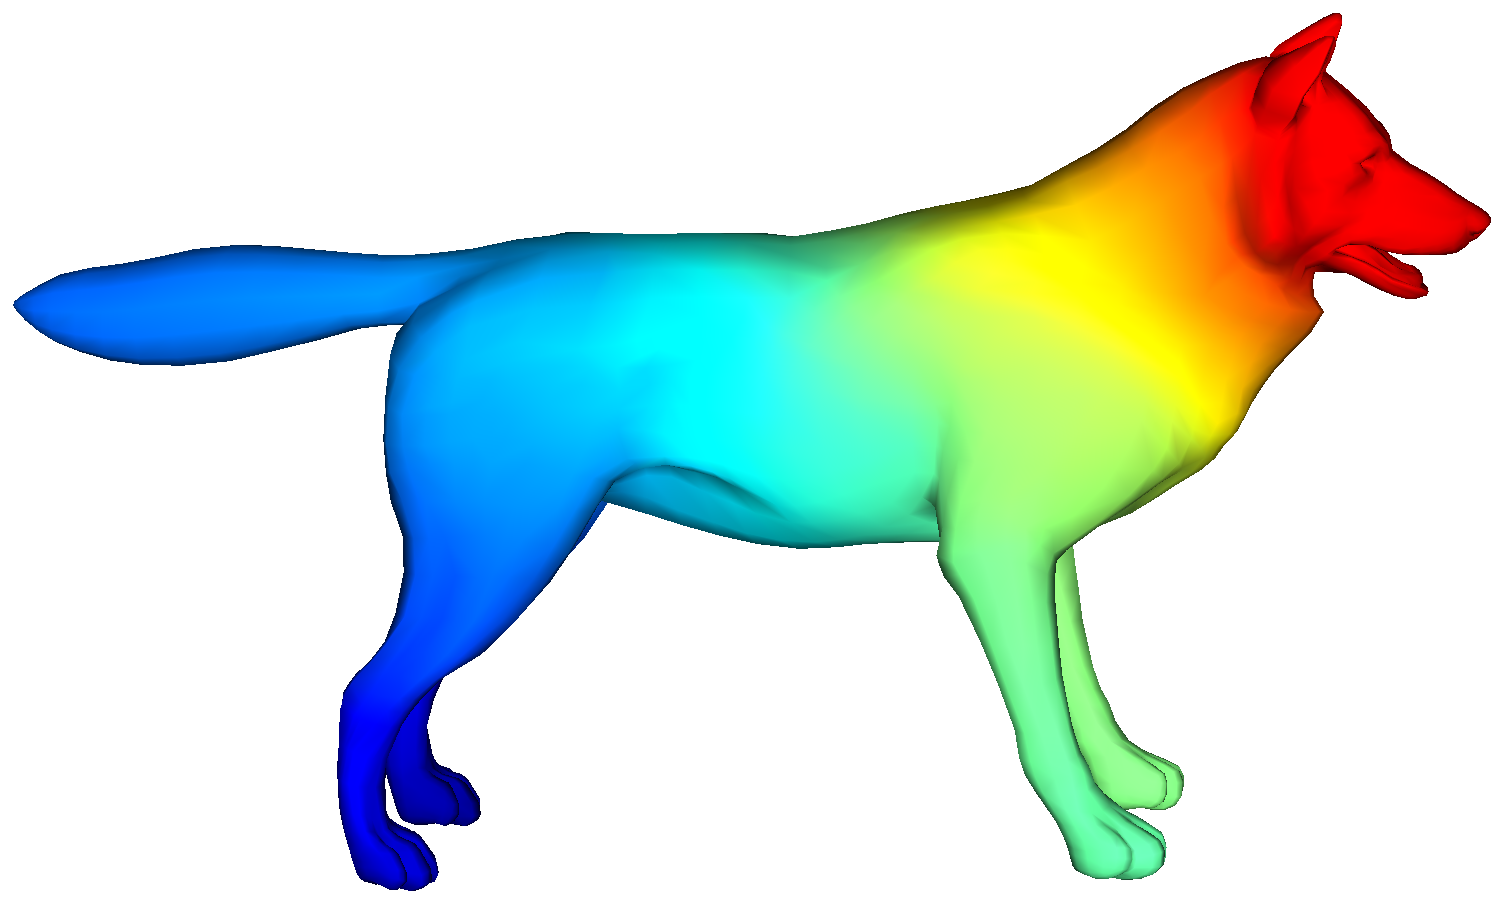
\includegraphics[width=\linewidth]{1}
                \caption{$\chi_1$}
                \label{fig:wolf_mhb_1}
        \end{subfigure}%
        ~
        \begin{subfigure}[b]{0.3\linewidth}
                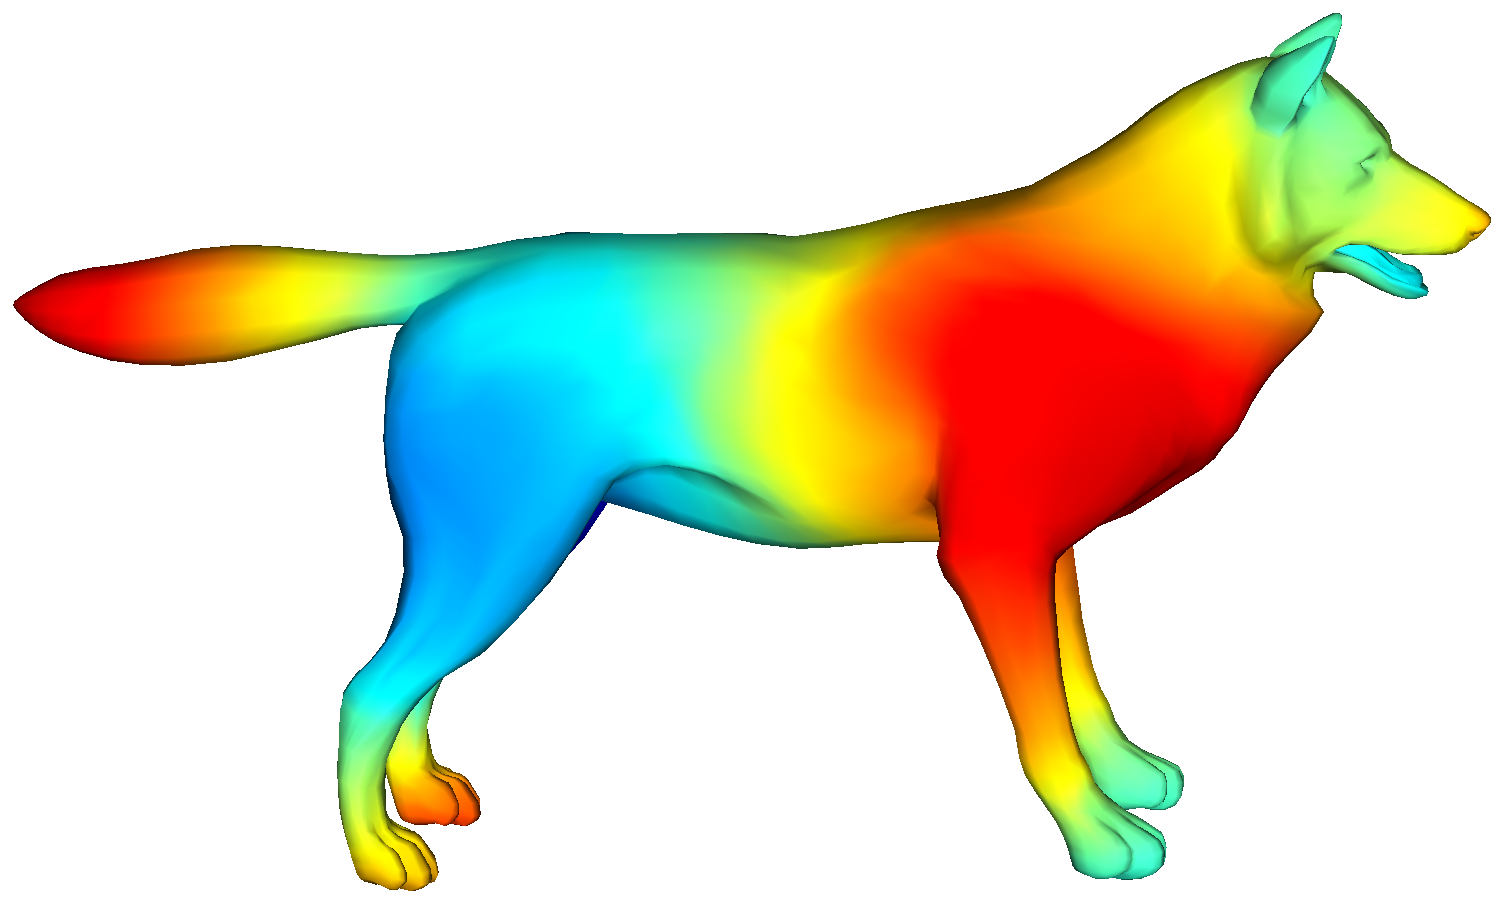
\includegraphics[width=\linewidth]{2}
                \caption{$\chi_{10}$}
                \label{fig:wolf_mhb_10}
        \end{subfigure}
        ~
        \begin{subfigure}[b]{0.3\linewidth}
                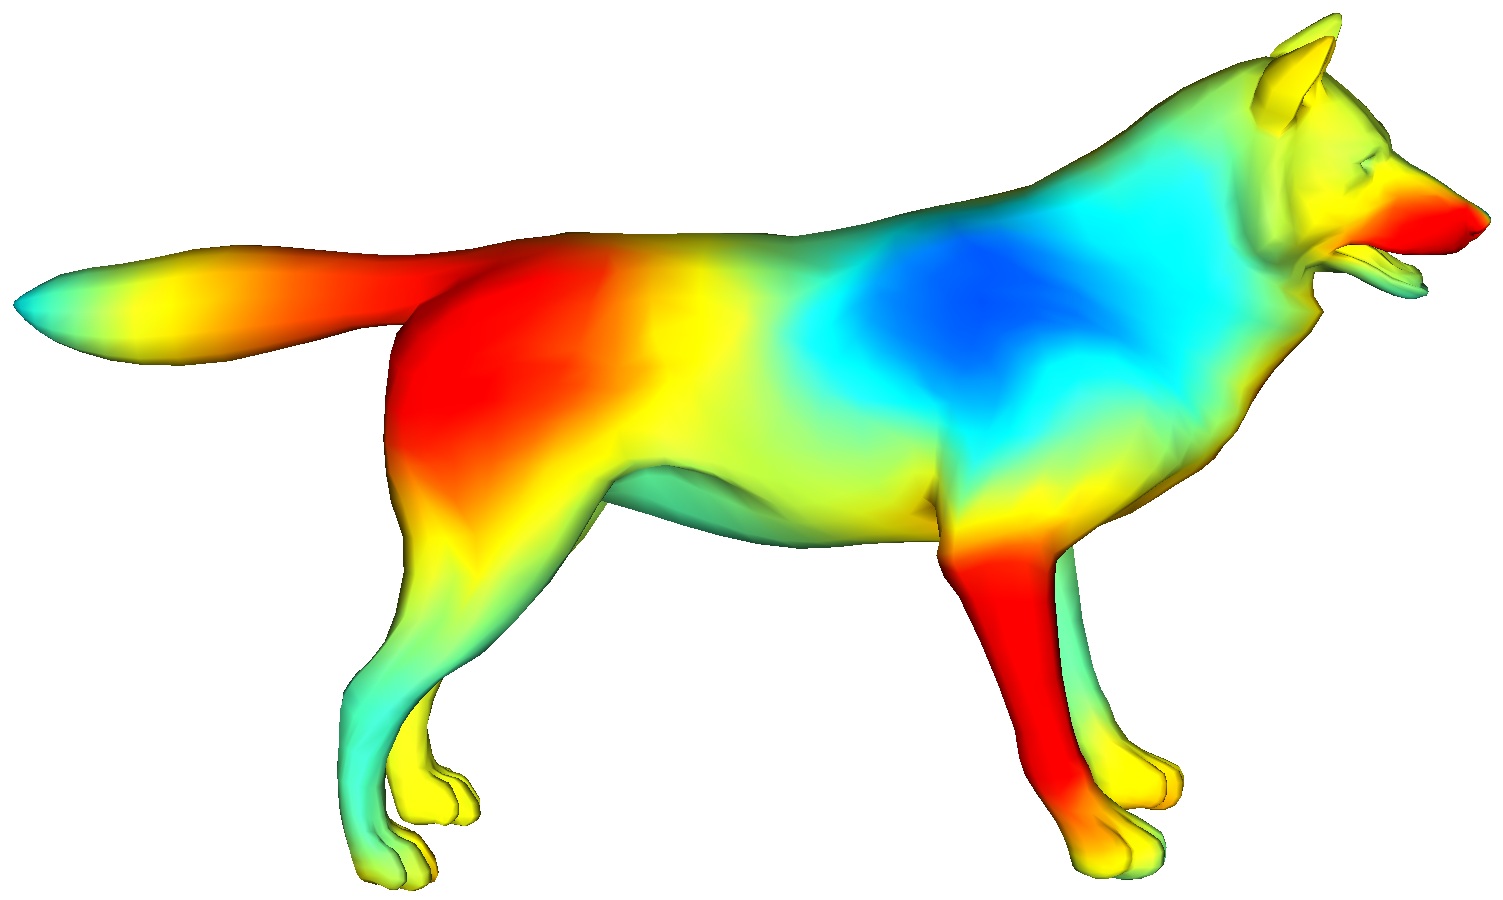
\includegraphics[width=\linewidth]{3}
                \caption{$\chi_{20}$}
                \label{fig:wolf_mhb_20}
        \end{subfigure}
        \caption[Visualization of MHBs.]
        {Visualization of the Laplacian eigenfunctions (MHB).
         From left to right, the first, tenth, and twentieth
         eigenfunctions are highlighted.}
        \label{fig:mhb}
\end{figure}

\subsection{Spectral Mesh Approximation via MHB}
\label{sec:mhbapprox}

The MHB can be employed to define the graph Fourier transform, also
known as the \emph{manifold harmonic transform} (MHT), which converts
a function between spatial domain and frequency domain. Any $f\in
L^2(M)$ can be expanded by MHB as
\begin{equation}
\label{eq:mht}
f = \sum_{k=0}^{n-1}\widehat{f}_k\phi_k = \sum_{k=0}^{n-1}\langle f,\phi_k\rangle\phi_k,
\end{equation}
in which $\widehat{f}_k$ is the $k$-th MHT coefficient of $f$.

The MHT is the theoretical foundation of the spectral mesh compression
proposed by Karni and Gotsman~\cite{Karni2000}. Viewing the
Euclidean mesh coordinates $\mathbf{x}$, $\mathbf{y}$ and $\mathbf{z}$
as functions defined on vertices, the basic idea of spectral
compression is to compute the MHT of the coordinate function and then
truncate out certain number of high-frequency coefficients. Take the
x-coordinate function $\mathbf{x}$ as an example. The original
coordinates can be perfectly recovered as in Eq.~(\ref{eq:mht}) if all
$n$ MHT coefficients $\{\widehat{x}_0,\ldots,\widehat{x}_{n-1}\}$ are
used. If we only retain the first $n'<n$ coefficients, the
reconstructed x-coordinate function $\mathbf{x'}=\sum_{k=0}^{n'-1}
\widehat{x}_k\phi_k$ is a low-pass-filtered version of $\mathbf{x}$
and can be regarded as an acceptable approximation. The reconstructed
mesh is smooth and the overall appearance tends to be very similar to
the original mesh, since low-frequency components, which correspond to
large-scale shape information, are prioritized to be preserved, and
our visual observations tend to be more forgiving to the loss of
high-frequency information.

Fig.~\ref{fig:fourier_approx} shows an example result of
spectral approximation using different number of MHB.
\begin{figure}
 \centering
 \begin{subfigure}[b]{0.23\linewidth}
  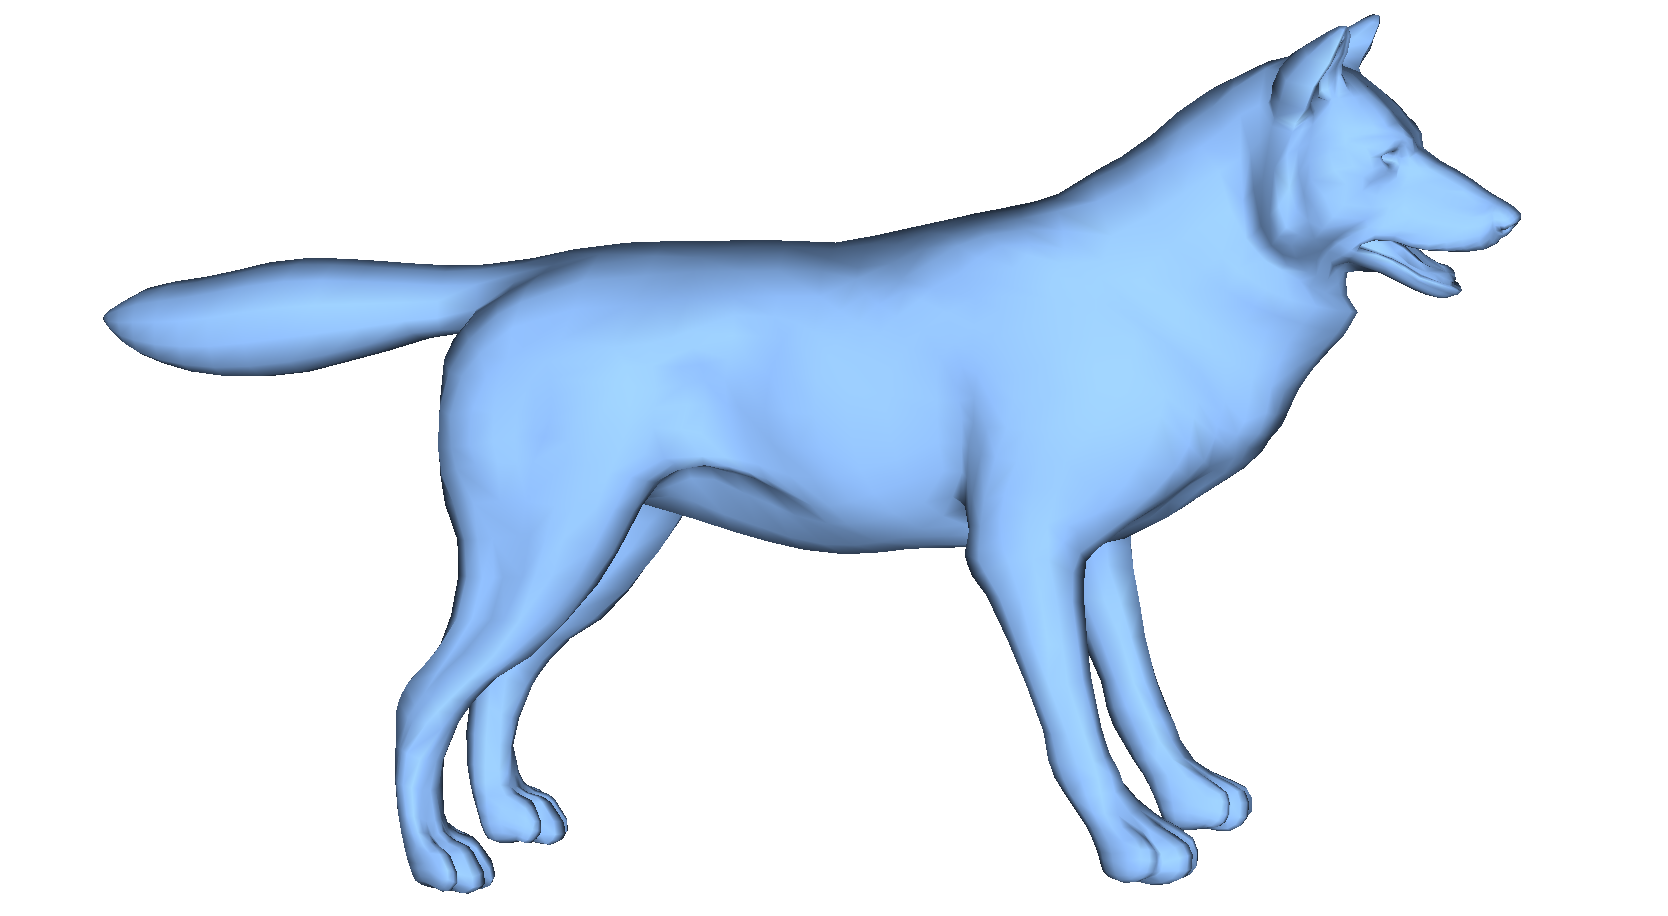
\includegraphics[width=\linewidth]{4}
  \caption{}
  \label{fig:fourier1}
 \end{subfigure}
 ~
 \begin{subfigure}[b]{0.23\linewidth}
  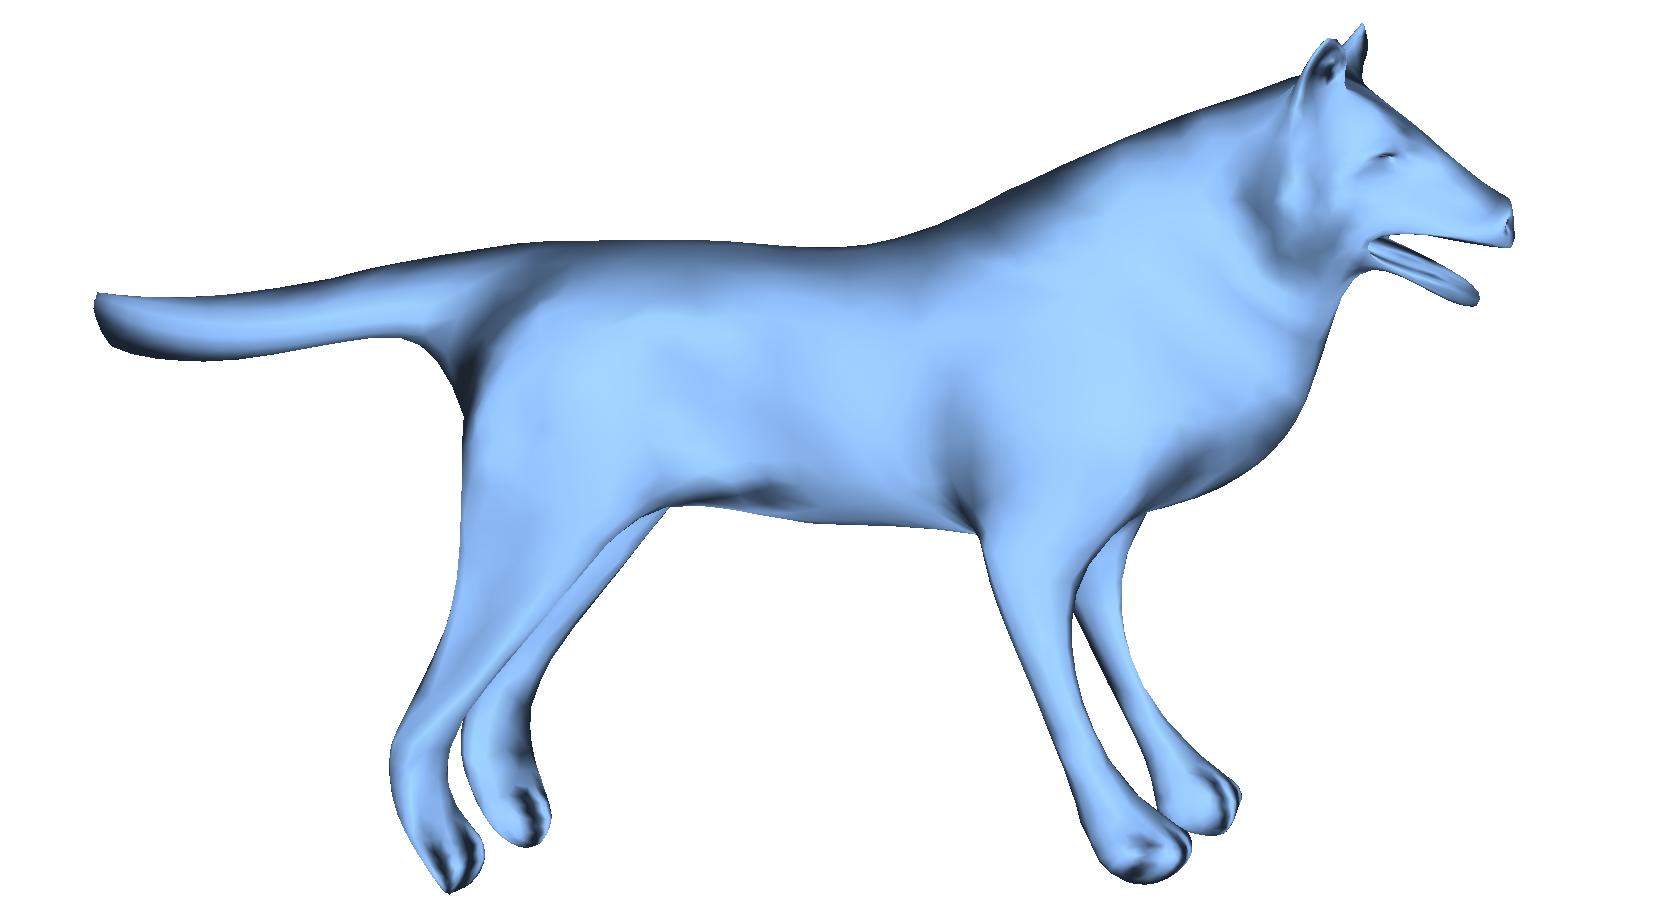
\includegraphics[width=\linewidth]{5}
  \caption{}
  \label{fig:fourier2}
 \end{subfigure}
 ~
 \begin{subfigure}[b]{0.23\linewidth}
  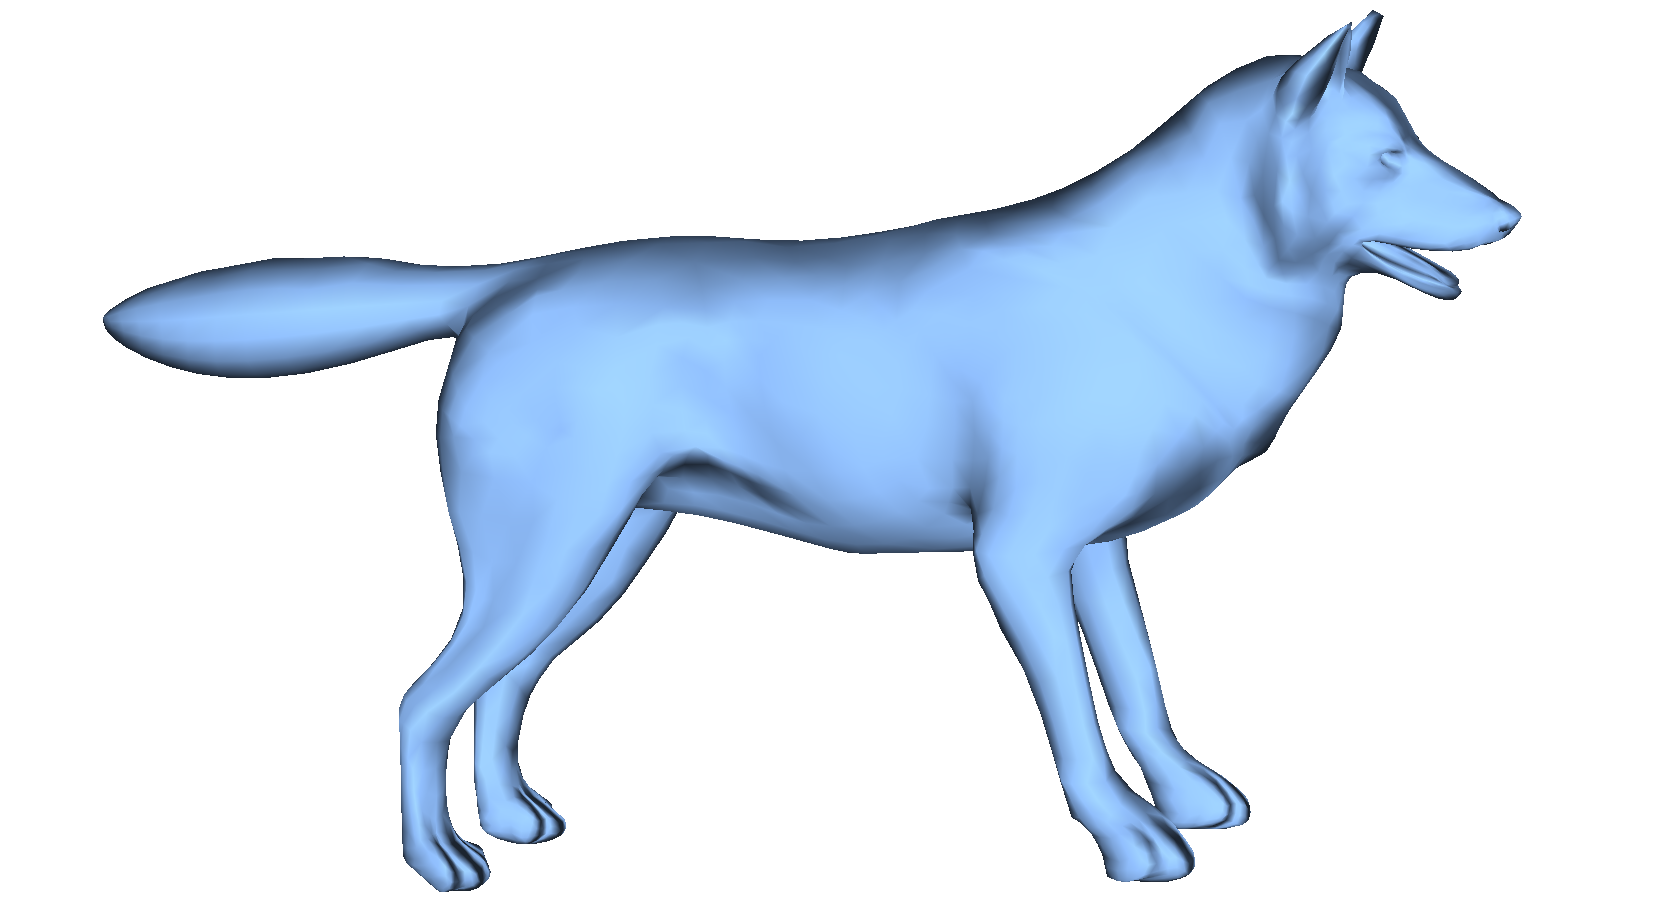
\includegraphics[width=\linewidth]{6}
  \caption{}
  \label{fig:fourier3}
 \end{subfigure}
 ~
 \begin{subfigure}[b]{0.23\linewidth}
  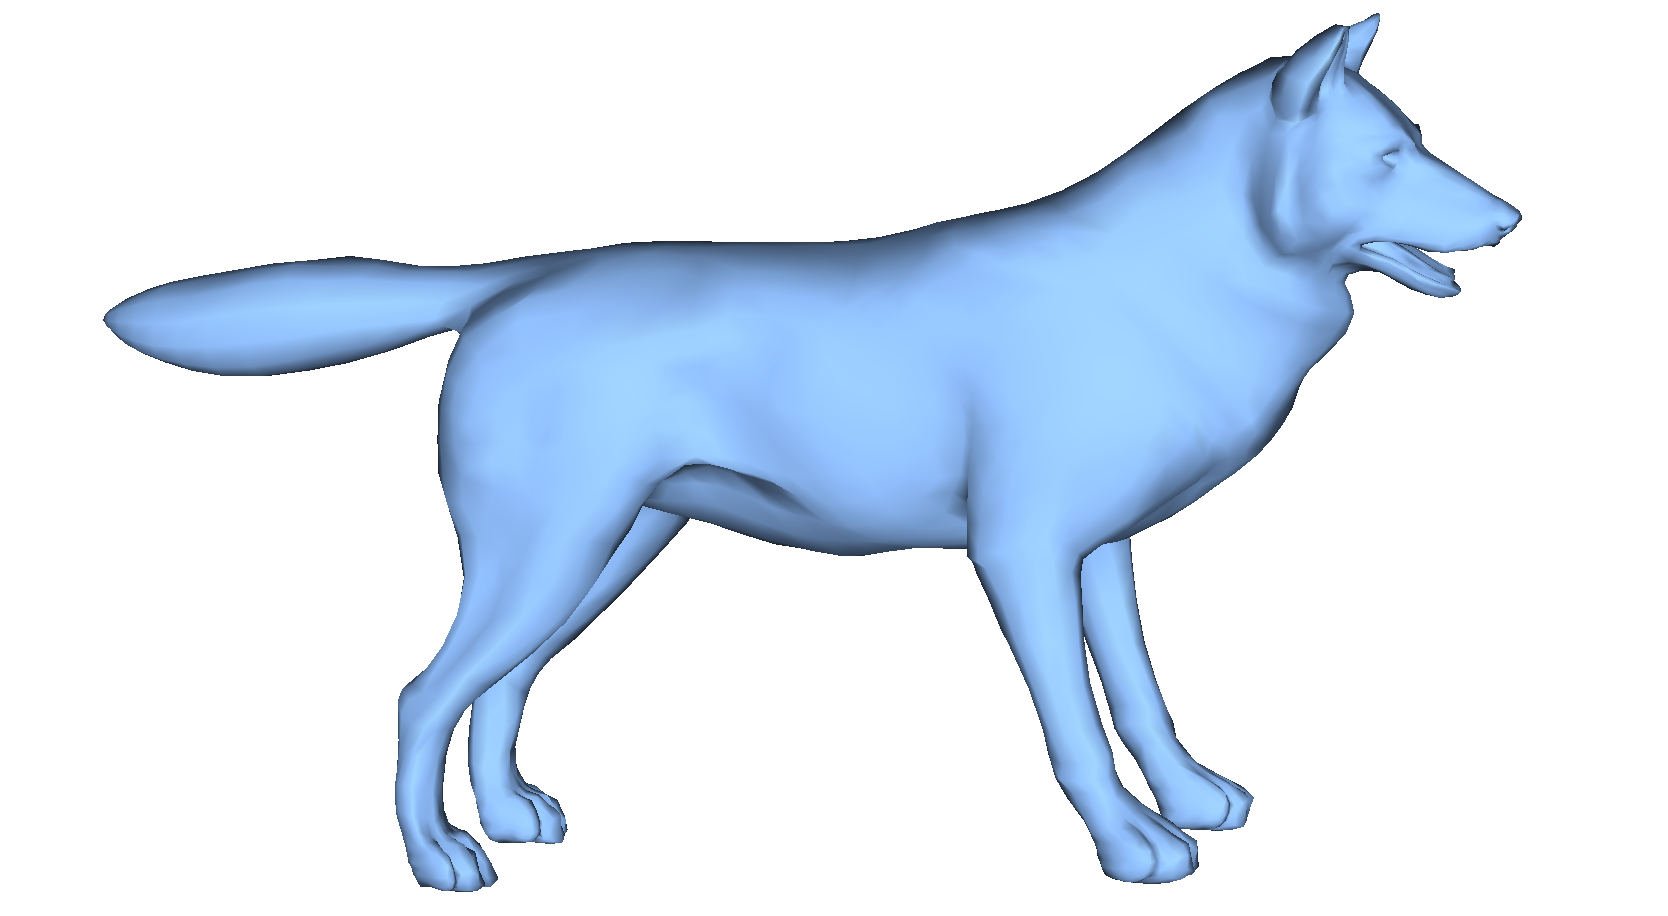
\includegraphics[width=\linewidth]{7}
  \caption{}
  \label{fig:fourier4}
 \end{subfigure}
 \caption[Spectral approximation of wolf model.]
 {Spectral approximation~\cite{Karni2000} of a 3D
  wolf model containing 4,344 vertices. (a) The original mesh. (b)
  Reconstruction using 100 eigenbases. (c) Reconstruction using 300
  eigenbases. (d) Reconstruction using 1000 eigenbases.}
 \label{fig:fourier_approx}
\end{figure}

\subsection{Spectral Graph Wavelets}
\label{sec:sgw}

The spectral graph wavelets (SGW), as described
in~\cite{Hammond2011}, are expressed as bivariate kernel
functions expanded on the MHB
\begin{equation}
\mathbf{\Psi_t}(i,j)=\sum_{k=0}^{n-1}g(t\lambda_k)\chi_k(i)\chi_k(j),
\end{equation}
where $g$ is the real-valued wavelet generator function and $t$ is the
scale parameter. The generator function $g$ modulates the spectral
wavelets in the frequency domain, and should satisfy the admissibility
condition
\begin{equation}
C_g=\int_0^{\infty}\frac{g^2(x)}{x}dx < \infty
\end{equation}
and $g(0)=0$. The $i$th row of $\Psi_t$
\begin{equation}
\psi_{t,i}(\cdot)=\sum_{k=0}^{n-1} g(t\lambda_k)\chi_k(i)\chi_k(\cdot)
\end{equation}
is the spectral wavelet spatially-localized at $v_i$, and in the
frequency domain, localized at scale $t$.

In practice, the scale parameter $t$ is discretized. The
spectral graph wavelets $\psi_{t,i}$ are near orthogonal to
$\chi_k$ for $\lambda_k$ near 0, i.e., low-frequency eigenbasis,
for any discrete scale $t$. Hence, to better capture low-frequency signal
information, \cite{Hammond2011} also introduced the \emph{spectral
scaling functions} which have similar constructions with SGW but act like low-pass filters
\begin{equation}
  \mathbf{\Phi}_t(i,j)=\sum_{k=0}^{n-1} h(t\lambda_k)\chi_k(i)\chi_k(j),
\end{equation}
in which the scaling generator function $h$ should satisfy $h(0)>0$
and $h(x)\rightarrow 0|_{x\rightarrow\infty}$.

Suppose we compute the spectral wavelets at $J$ different scales
$\{t_1,t_2,\ldots,t_J\}$, the constructed SGW then comprises
$(J+1)\times n$ functions in $\mathbb{R}^n$. In this chapter, we adopt
the same formulation of wavelet and scaling functions used
in~\cite{Hammond2011} with the generator function
\begin{equation}
g(x)=
\begin{cases}
        x^2 & \text{if } x<1\\
        -5+11x-6x^2+x^3 & \text{if } 1\leq x \leq 2\\
        4x^{-2} & \text{if } x>2.
    \end{cases}
\end{equation}
The $J$ scales are selected to be logarithmically equally spaced
between the minimum scale $t_J=2/\lambda_{max}$ and the maximum scale
$t_1=40/\lambda_{max}$, where $\lambda_{max}$ is the upper bound of
the Laplacian eigenvalues. For the scaling function, the generator is
$h(x)=\gamma\exp(-(\frac{20x}{0.6\lambda_{max}})^4)$, in which
$\gamma=h(0)$ equals the maximum value of $g$.

Fig.~\ref{fig:sgw} visualizes multiscale spectral graph wavelets on a
3D mesh. It may be noted that, the values of wavelets are attenuated
and oscillating on the mesh, and wavelets with a larger scale have a
wider oscillating window.
\begin{figure}
\centering
\begin{subfigure}[b]{0.3\linewidth}
    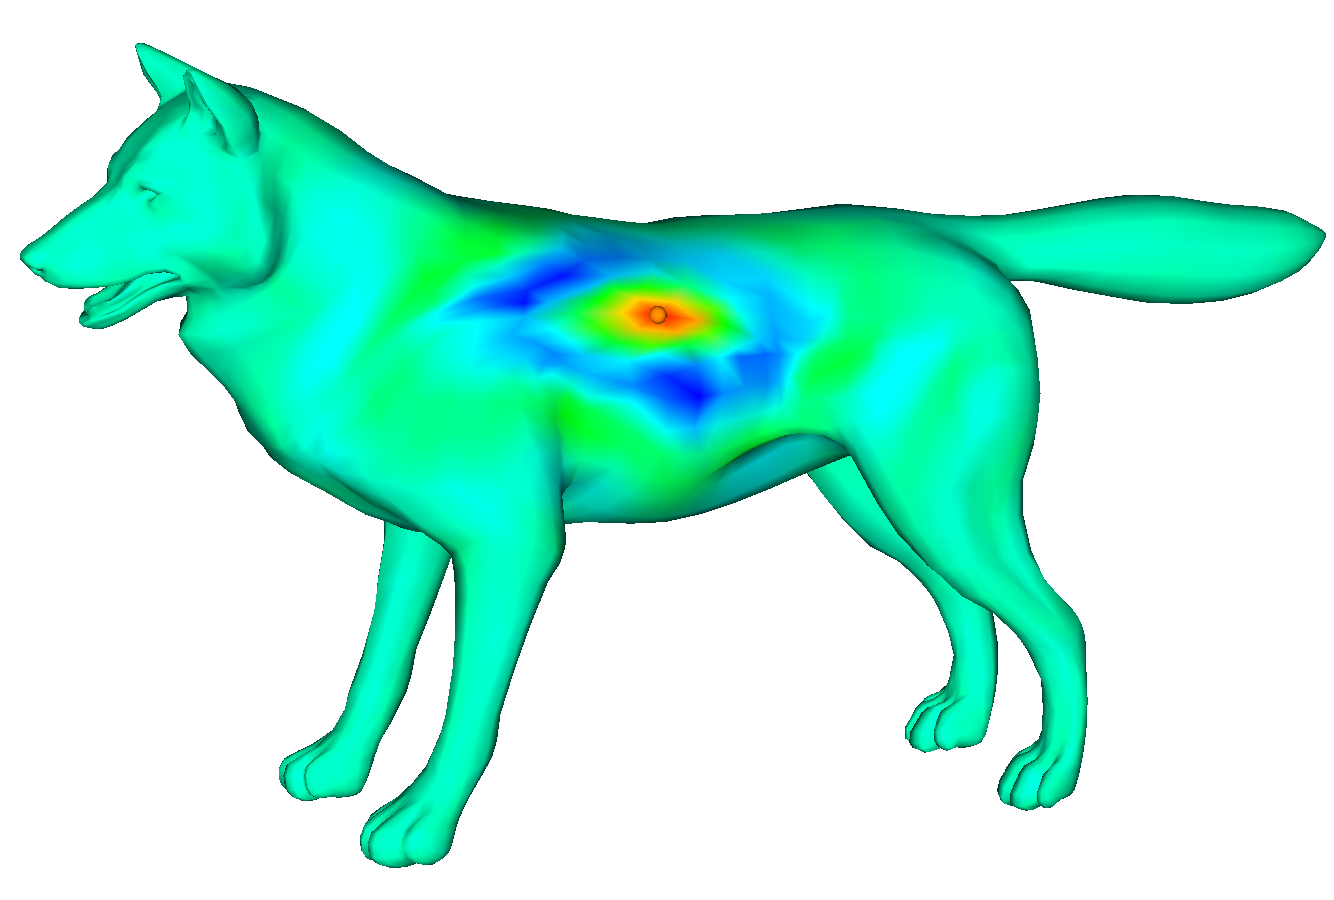
\includegraphics[width=\linewidth]{8}
    \label{fig:sgw1}
\end{subfigure}%
~
\begin{subfigure}[b]{0.3\linewidth}
    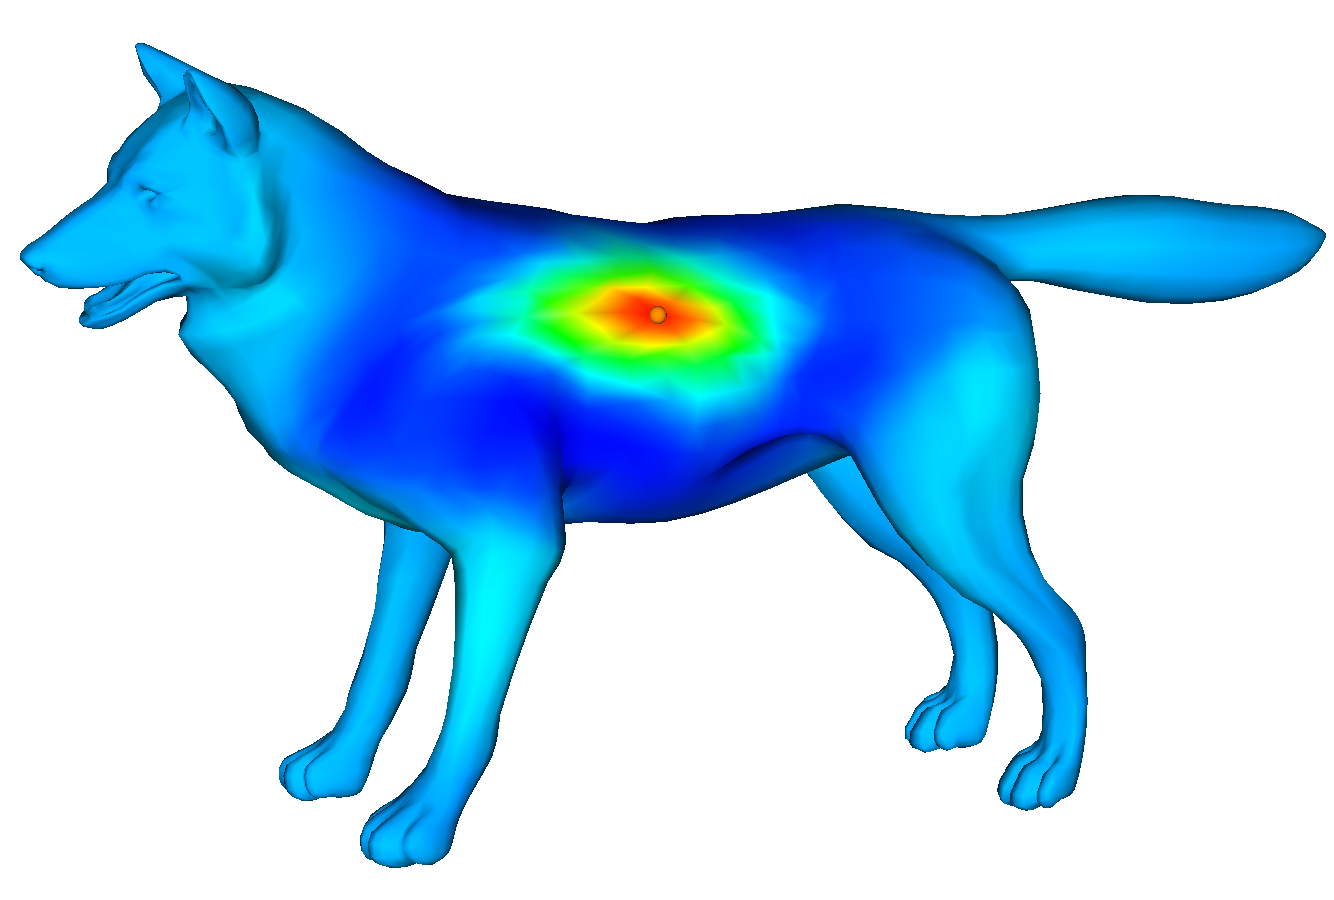
\includegraphics[width=\linewidth]{9}
    \label{fig:sgw2}
\end{subfigure}
~
\begin{subfigure}[b]{0.3\linewidth}
    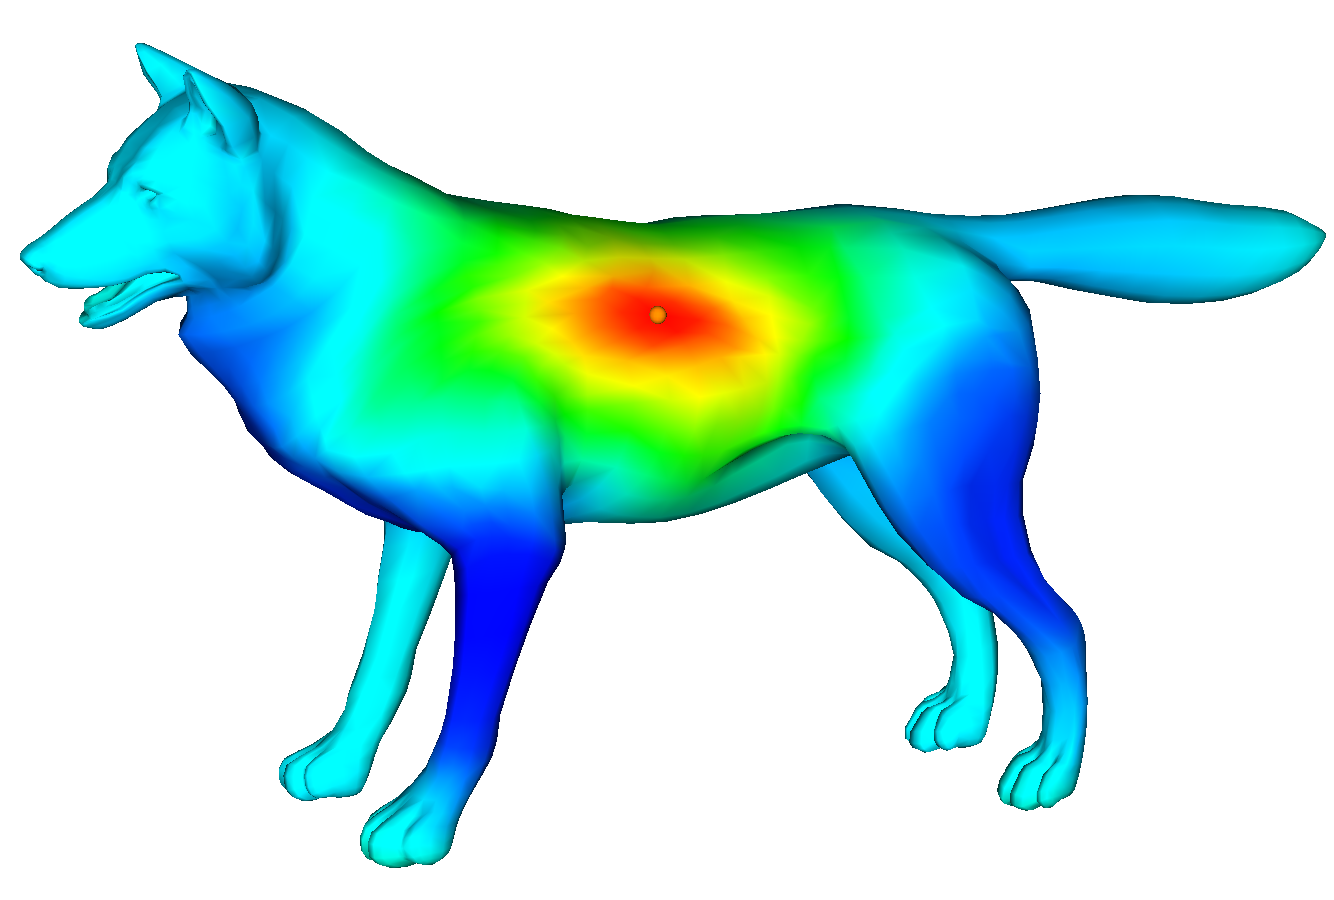
\includegraphics[width=\linewidth]{10}
    \label{fig:sgw3}
\end{subfigure}%
\caption[Visualization of spectral graph wavelets with different scales.]
{Visualization of spectral graph wavelets localized at the
 same point but with different scales. From left to right, the
 spectral wavelets at scale 1, 3, and 5 are highlighted.}
\label{fig:sgw}
\end{figure}

In Sec.~\ref{sec:mhbapprox} we have shown that the mesh coordinates
can be transformed into the frequency domain via MHT using the
Laplacian eigenbasis, and compression can be achieved by trimming out
a user-specified number of high-frequency coefficients. The main
drawbacks of this naive and simple low-pass spectral compression
method are: (1) It innately favors low-frequency information while
most high-frequency geometric details are compromised; (2) The
Laplacian eigenbasis, which serve as the compression dictionary, all
have global support and therefore are not efficient in encoding local
geometry.

In this chapter, we propose to use SGW to construct a redundant
dictionary. Because of its powerful property of spatial localization,
the multiscale SGW functions are much more efficient in representing
local mesh geometry around individual vertices than the Laplacian
eigenbasis. Since the size of SGW dictionary is much larger than the
number of mesh vertices, we employ powerful sparse approximation
algorithms to find a compact representation which selects the most
appropriate basis in the procedure.

\subsection{Sparse Approximation of Mesh Coordinates}

For mesh $M$, let $\mathbf{D}$ be a dictionary of $L^2(M)$ containing
$m$ normalized basis vectors. The dictionary can be written as a
$n\times m$ matrix $\mathbf{D} = \begin{pmatrix} \mathbf{a_1} &
  \mathbf{a_2} & \ldots & \mathbf{a_m} \end{pmatrix}$, where
$\mathbf{a_i} \in \mathbb{R}^{n\times 1}$. Our aim is to approximate
function $\mathbf{y}\in L_2(M)$ with a linear combination of the atoms
in $\mathbf{D}$, expressed in the matrix form as
$\widehat{\mathbf{y}}=\mathbf{D}\mathbf{x}=\sum_{i=1}^m
x_i\mathbf{a_i}$. Here the vector $\mathbf{x}\in\mathbb{R}^m$ is the
coefficient representation of the input signal $\mathbf{y}$ w.r.t. the
dictionary $\mathbf{D}$.

An effective compression of the original signal $\mathbf{y}$ requires
the number of elementary signals that participate in the linear
combination to be small and the reconstructed result
$\widehat{\mathbf{y}}$ to be as close to $\mathbf{y}$ as possible. In
principle, the number of non-zero elements of the coefficient vector
$\mathbf{x}$, denoted by the pseudo-norm $\|\mathbf{x}\|_0$, should
satisfy $\|\mathbf{x}\|_0 \ll n$ in order to achieve significant
reduction in storage. Fixing the number of participating atoms in the
sparse approximation to be $n'$, the problem to produce the optimal
sparse representation $\mathbf{x}$ can be formulated as:
\begin{equation}
  \min_{\mathbf{x}} \|\mathbf{y}-D\mathbf{x}\|_2^2\ \textrm{subject\ to}\ \|\mathbf{x}\|_0 = n'.
\label{eq:sa}
\end{equation}

If the input signal has $c$ channels, denoted as a $n\times c$ matrix
$\mathbf{Y}=(\mathbf{y_1},\mathbf{y_2},\ldots,\mathbf{y_c})$, the
coefficient representation should be a $m\times c$ matrix
$\mathbf{X}=(\mathbf{x_1},\ldots,\mathbf{x_c})$ satisfying $\mathbf{Y}
\approx \mathbf{D}\mathbf{X}$. We may either treat each channel
(column) of $\mathbf{Y}$ independently and select different subsets of
participating atoms for each channel, or use the same subset for all
the channels and minimize the combined approximation errors. The
latter one is called the \emph{simultaneous sparse approximation} problem
\begin{equation*}
  \min_{\mathbf{X}} \|\mathbf{Y}-\mathbf{D}\mathbf{X}\|_F^2
\end{equation*}
subject to
\begin{equation}
\begin{cases}
    support(\mathbf{x_1})=\cdots=support(\mathbf{x_c})\\
    \|\mathbf{x_1}\|_0=\cdots=\|\mathbf{x_c}\|_0=n',
\end{cases}
\label{eq:simulsa}
\end{equation}
where $\|\cdot\|_F$ is the Frobenius norm, and $support(\mathbf{x_i})$
denotes the index set of non-zero elements in $\mathbf{x_i}$.

The vertex coordinates of a mesh can be treated as a 3-channel signal
$p(\mathbf{v})=(\mathbf{v_x}, \mathbf{v_y}, \mathbf{v_z})$. Since the
three coordinate functions are correlated, it is preferable to
formulate the mesh compression as the simultaneous sparse
approximation problem. Determining the optimal solution to
Eq.~(\ref{eq:simulsa}) is NP-hard, but we can find approximate
solutions using greedy pursuit algorithms such as the
\emph{simultaneous orthogonal matching pursuit} (S-OMP)
\cite{Tropp2006a}. The key idea is to iteratively select
from the dictionary a new atom that has the best correlation with the
residual shape, and then project the original mesh onto the space
spanned by the selected atoms to obtain a new approximate shape.
Please refer to Algorithm~\ref{alg:somp} for details.
\begin{algorithm}
\caption{S-OMP on 3D mesh coordinates.}
\label{alg:somp}
\begin{algorithmic}
\STATE \textbf{Input:}
\STATE \begin{itemize}
         \item 3D mesh coordinates $\mathbf{S}\in\mathbb{R}^{n\times 3}$.
         \item Dictionary $\mathbf{D}=\{\mathbf{a_1},\mathbf{a_2},\ldots,\mathbf{a_m}\}, \mathbf{a_i}\in\mathbb{R}^3$.
         \item The number of atoms to be selected $n'$.
       \end{itemize}
\STATE \textbf{Initialization:}
\STATE \begin{itemize}
         %\item The index set of all atoms $\Omega=\{1,2,\ldots,m\}$.
         \item The initial index set of selected atoms $\Lambda_0=\emptyset$.
         \item The initial residual $\mathbf{R_0}=\mathbf{S}$;
         \item The iteration counter $t=1$.
       \end{itemize}
\STATE \textbf{Procedure:}
\STATE (1) Find an index $i_t$ of $\mathbf{D}$ that satisfies
    $$ i_t = \argmax_{j\not\in\Lambda_{t-1}} \sum_{k=1}^3 |\langle \mathbf{R_{t-1}}\mathbf{e_k}, \mathbf{a_j} \rangle|, $$
    where $e_k$ denotes the $k$th canonical basis vector in $\mathbb{R}^3$.
\STATE (2) Set $\Lambda_t=\Lambda_{t-1}\bigcup\{i_t\}$.
\STATE (3) Compute the coefficient matrix $\mathbf{C_t}$ by solving the least-square problem
    $$ \mathbf{C_t}=\argmin_{\mathbf{X}}=\|\mathbf{S}-\mathbf{D}\mathbf{\mathbf{X}}\|_2^2$$
    subject to $support(X)=\Lambda_t.$
\STATE (4) Calculate the new approximation and residual:
    $$ \mathbf{\widehat{S}_t} = \mathbf{D}\mathbf{C_t}, $$
    $$ \mathbf{R_t} = \mathbf{S} - \mathbf{\widehat{S}_t}. $$
\STATE (5) Stop if $t=n'$. Otherwise, increment $t$ and go to (1).
\STATE \textbf{Output:}
\STATE \begin{itemize}
         \item The index set of selected atoms $\Lambda_{n'}$.
         \item Final coefficient matrix $\mathbf{C_{n'}}$.
        \end{itemize}
\end{algorithmic}
\end{algorithm}

We may also adopt the \emph{simultaneous matching pursuit} (S-MP) algorithm
which can be viewed as a simplification of S-OMP. The main difference from S-OMP is
the omission of the step to update all existing coefficients by orthogonal projection.
If all atoms in $\mathbf{D}$ are mutually orthogonal (e.g., Fourier dictionary), S-MP and S-OMP
will produce exactly the same result.

\subsection{Dictionary Design Strategies}
\label{sec:dictionary}

The key to effective sparse approximation is the selection of
elementary functions that form the dictionary. A natural choice is the
MHB dictionary composed entirely of Laplacian eigenbasis
$\{\chi_0,\chi_2,\ldots,\chi_{n-1}\}$. The MHB functions have global
support and multiple frequencies, making the MHB dictionary a good
choice for encoding a shape when global, periodical, and symmetric
information is prioritized to be preserved. In addition, since MHB are
orthogonal basis, we can replace orthogonal matching pursuit (OMP)
with the much faster matching pursuit (MP) and the approximation
results will be the same.

However, MHB dictionary is very inefficient in capturing
non-periodical, local details due to the global support. It is
desirable to have a dictionary with a class of functions that have
local support but are still smooth and multiscale. In this work, we
propose to use normalized multiscale SGW, as described in
Sec.~\ref{sec:sgw}, as atoms to construct the dictionary for sparse
approximation. The SGW dictionary has several advantages:
\begin{itemize}
\item The SGW atoms are compact and localized at vertices, suitable
  for encoding local geometric features.
\item The SGW atoms can cover multiple scales, enabling the efficient
  representation of both small-scale and large-scale shape information
  in the vincinity of each vertex.
\item The computation of SGW from MHB is straightforward, and can be
  done on the decoder side provided the mesh connectivity is known.
\end{itemize}

On the flip side, the SGW are less efficient than MHB for encoding
global shape structures. Moreover, since SGW functions always have
extreme values at their origin vertices, a mesh reconstructed from SGW
atoms may exhibit unpleasant protrudes at vertices where selected SGW
are centered, which can be further ameliorated by constructing a
dictionary that contains both MHB and SGW. The mixed dictionary
potentially inherits the advantages of both waveforms, at the cost of
increased dictionary size.

The SGW or SGW+MHB dictionary are non-orthogonal and redundant,
forcing us to use costly sparse approximation methods such as S-OMP.
The enlarged dictionary also increase the storage requirements for the
dictionary themselves and for the sparse coefficient representation
(see Sec.~\ref{sec:compratio}).

Fig.~\ref{fig:wolf} shows an example of sparse approximation results
using three methods: (1) Spectral mesh compression via MHB, as
described in Sec.~\ref{sec:mhbapprox}; (2) S-MP with the MHB
dictionary; (3) S-OMP with the SGW dictionary. In this example, the
S-MP method produces higher-quality shape approximation than the naive
low-pass spectral approximation using the same MHB dictionary.
Adopting the multiscale SGW dictionary in place of MHB further
improves the approximation results. In particular, the SGW dictionary
are more effective in preserving local geometric features, while
MHB-based approximations have the tendency to smooth out some body
parts such as the wolf's legs when the number of participating bases
is small.

\begin{figure}
    \centering
    \includegraphics[width=\linewidth]{11}
    \caption[Comparison of three approximation methods.]
    {Comparison of the approximation results of three
      different approximation methods. \emph{Top row}: Spectral
      compression by truncating MHB coefficients. \emph{Second row}:
      S-MP approximation with MHB bases. \emph{Bottom row}: S-OMP
      approximation with SGW bases. For each method, from left to
      right, the number of participating bases are 20, 50, and 100,
      respectively.}
    \label{fig:wolf}
\end{figure}

\subsection{Compression Ratio and Analysis}
\label{sec:compratio}

Now we analyze the compression ratio of the simultaneous sparse
representation using a simple coding scheme. Assume the dictionary $D$
are known in advance on both the encoder and decoder sides. The sparse
$m\times 3$ coefficient matrix $\mathbf{X}$ contains $n'$ non-zero
rows, and can be conveniently expressed by $3n'$ non-zero values and a
vector of size $n'$ specifying the indices of corresponding atoms. For
a dictionary containing $m$ atoms, each index occupies $\lceil\log_2
m\rceil$ bits, and the total cost to store the index vector is
$n'\lceil\log_2 m\rceil$. If the sparsity of $\mathbf{X}$, namely the
ratio of non-zero elements, is greater than $1/\lceil\log_2 m\rceil$,
it would be more efficient to represent the non-zero positions with a
bit-vector of size $m$. Assuming each signal element in $\mathbf{Y}$
takes up $k$ bits, and each coefficient in $\mathbf{X}$ requires $k'$
bits to store, the storage size of the original 3D coordinates is then
$3nk$ bits. The effective compression ratio is
\begin{equation}\label{eq:compress}
\Gamma = \frac{3n'k' + \min (m, n'\lceil\log_2 m\rceil}{3nk}.
\end{equation}

Assume that the dictionary contains $m=\alpha n$ atoms, and both the
coordinates and coefficients are stored in single-precision $k=k'=32$,
the compression ratio is then
\begin{equation}\label{eq:compress2}
  \Gamma = \frac{n'}{n} + \min(\frac{\alpha}{96}, \frac{n'\lceil\log_2\alpha n\rceil}{96n}).
\end{equation}
In comparison, the compression ratio of the coefficient truncation
method introduced in Sec.~\ref{sec:mhbapprox} is simply $n'/n$ with
$n'$ coefficients, since there is no need to store the indices of
non-zeros.

From Eq.~(\ref{eq:compress2}) we can easily see that enlarging the
dictionary (larger $\alpha$) increases the overhead ratio for a given
mesh. In addition, when the coefficient matrix is very sparse, the
overhead ratio becomes smaller for larger meshes, since $log_2\alpha
n$ increases slower than $n$.

\subsection{Mesh Partitioning}
\label{seq:partition}

The most time-consuming part of S-OMP is to compute the maximum inner
product between the residual and available atoms, which costs $O(mn)$
in each iteration. In principle, the required number of iterations
$n'$ and the size of dictionary $m$ are linearly proportional to the
mesh size $n$, hence the total time complexity is $O(n^3)$, which is
unacceptable for very large meshes. In addition, all the dictionaries
we use are constructed from the eigenvectors of mesh Laplacian, but
the full Laplacian eigendecomposition of a large mesh is very time
consuming and can be numerically instable. Hence, when the input mesh
is very large, it is necessary to perform graph partitioning and carry
on the compression algorithm on each individual sub-mesh. As suggested
in~\cite{Karni2000}, we use the METIS package~\cite{karypis1998fast}
which implements several fast graph partitioning algorithms.

On the other hand, as mentioned in Sec.~\ref{sec:compratio}, the
overhead for storing the indices of selected atoms is smaller when the
mesh size becomes larger. Moreover, increasing the number of
sub-meshes also increases the occurrences of unpleasant artifacts
along sub-mesh boundaries. Thus, a tradeoff needs to be made between
the compression time and quality. In our implementation, a large mesh
is decomposed into a number of patches containing approximately equal
number of vertices, with the maximum patch size set to be 1,000.


\section{Experimental Results}

\subsection{Evaluation Method}

To evaluate the effectiveness of lossy mesh compression methods, we
adopt the mesh comparison metric proposed
in~\cite{Karni2000} to measure the errors between the
original mesh geometry and approximate ones. Let $M_1$ and $M_2$ be
two meshes to be compared, both containing $n$ vertices, and
$\mathbf{v^1_i}$ and $\mathbf{v^2_i}$ denote the 3D coordinates of the
$i$-th vertex in $M_1$ and $M_2$, respectively. The \emph{geometric
  error} between $M_1$ and $M_2$ is
\begin{equation}
  \|M_1-M_2\|_g = \sum_{i=1}^n \frac{1}{n}\|{\mathbf{v^1_i}-\mathbf{v^2_i}}\|_2.
\end{equation}
To better capture visual closeness such as smoothness,
\cite{Karni2000} introduces another metric which measures
the errors after applying the geometric Laplacian to mesh coordinates,
i.e., transforming the absolute coordinates to differential coordinates
\begin{equation}
  GL(\mathbf{v_i})=\mathbf{v_i}-\frac{\sum_{j\in N(i)}l_{ij}^{-1}\mathbf{v_j}}{\sum_{j\in N(i)}l_{ij}^{-1}},
\end{equation}
where $l_{ij}$ represents the edge length between $v_i$ and $v_j$. The
\emph{differential error} between $M_1$ and $M_2$ is then defined as
\begin{equation}
  \|M_1-M_2\|_d=\sum_{i=1}^n \frac{1}{n}\|GL(\mathbf{v^1_i})-GL(\mathbf{v^2_i})\|_2.
\end{equation}
The final error metric is the average of geometric error and
differential error
\begin{equation}
\|M_1-M_2\|=\frac{1}{2}(\|M_1-M_2\|_g + \|M_1-M_2\|_d).
\label{eq:metric}
\end{equation}

\subsection{Compression Performance}

\begin{figure}
    \centering
    \begin{subfigure}{0.4\linewidth}
        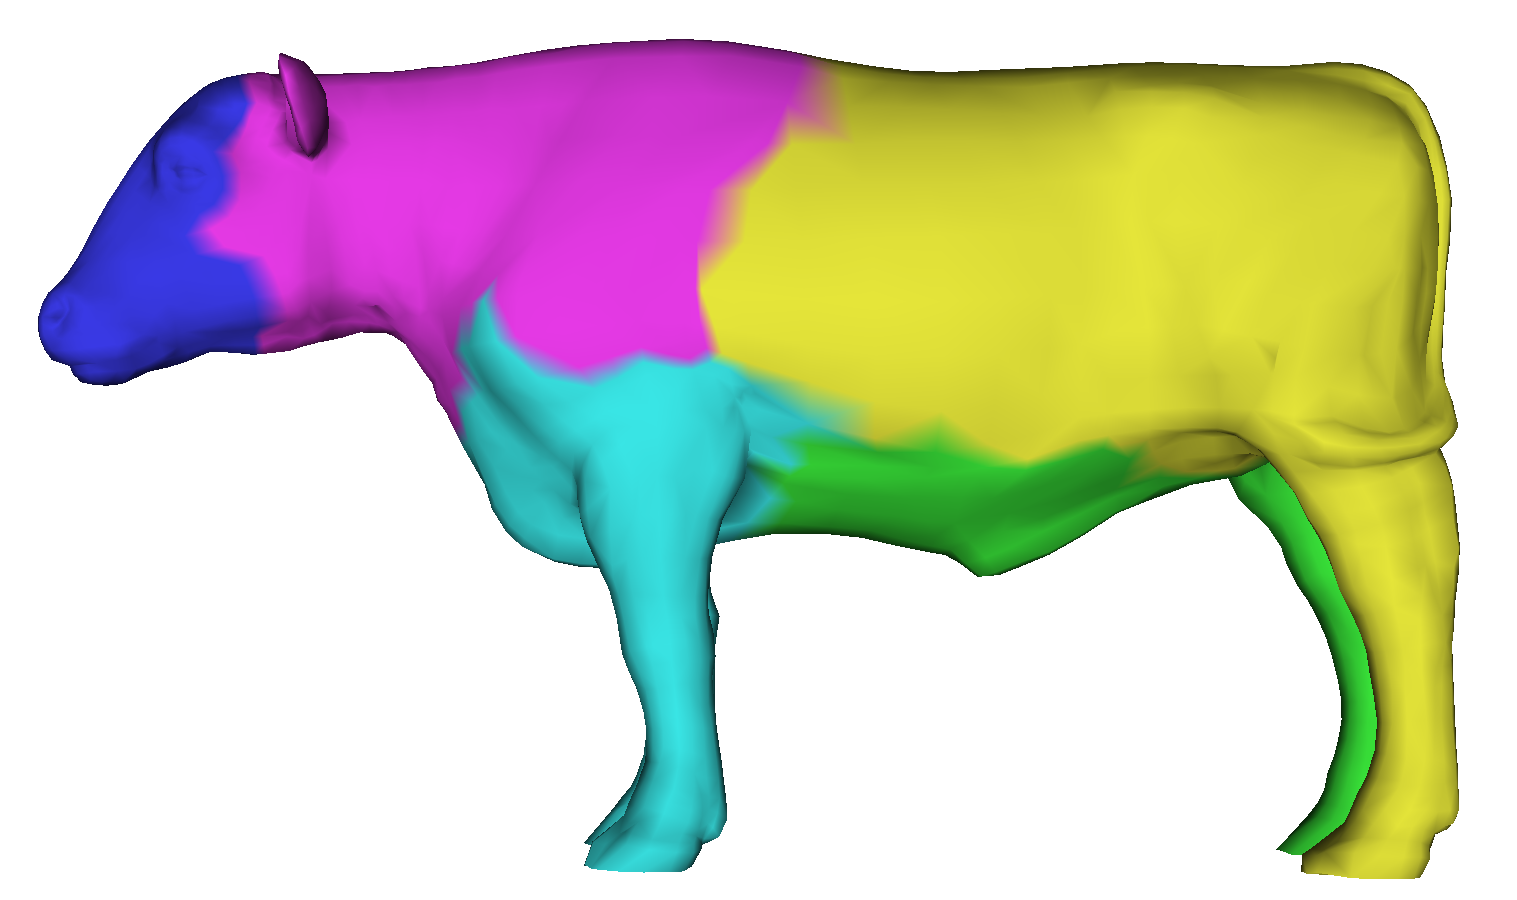
\includegraphics[width=\linewidth]{12}
        \caption{}
    \end{subfigure}
    ~
    \begin{subfigure}{0.4\linewidth}
        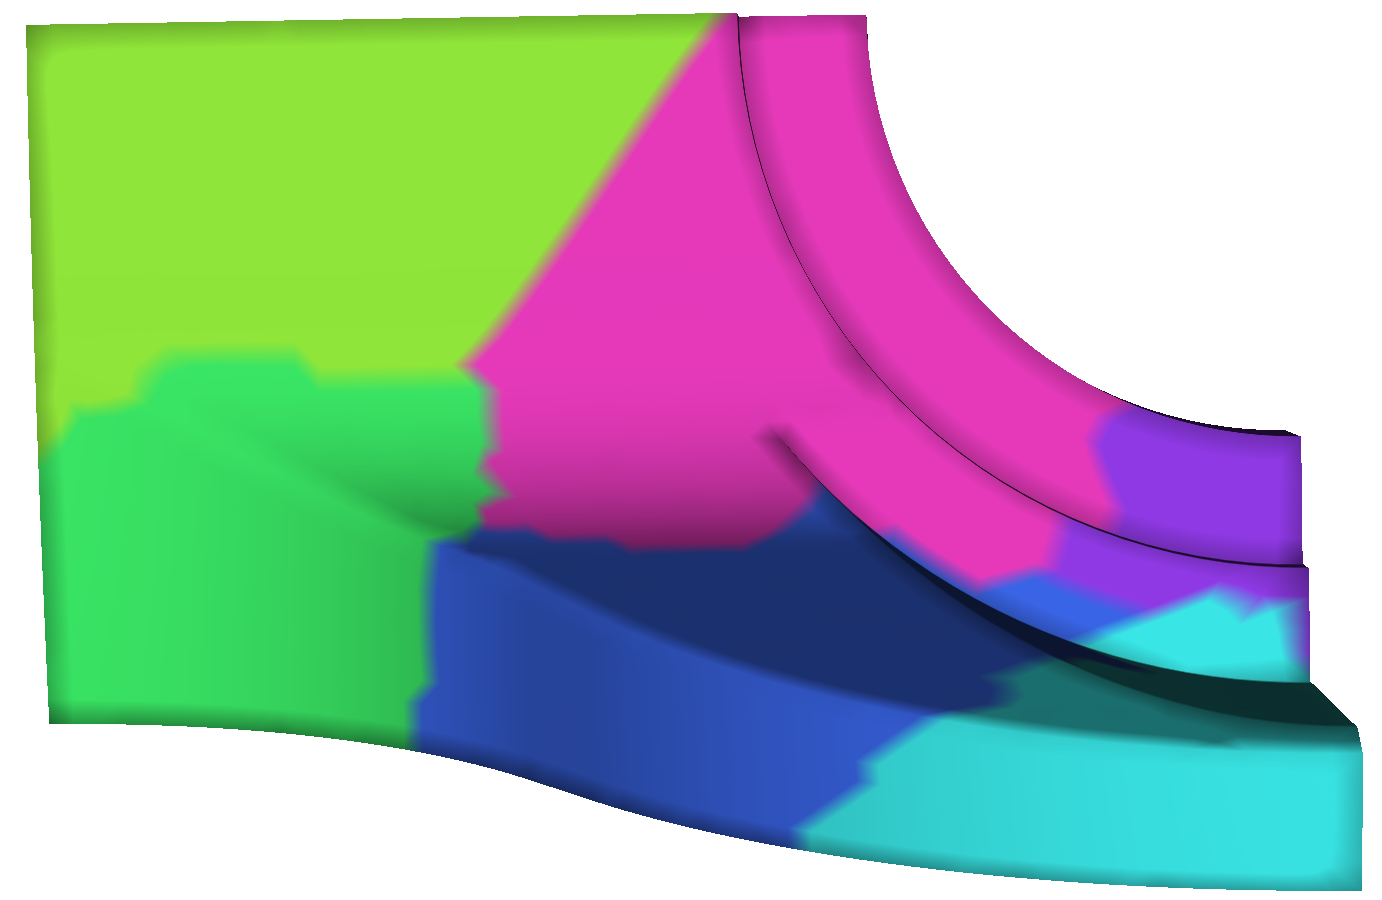
\includegraphics[width=\linewidth]{13}
        \caption{}
    \end{subfigure}
    ~
    \begin{subfigure}{0.4\linewidth}
        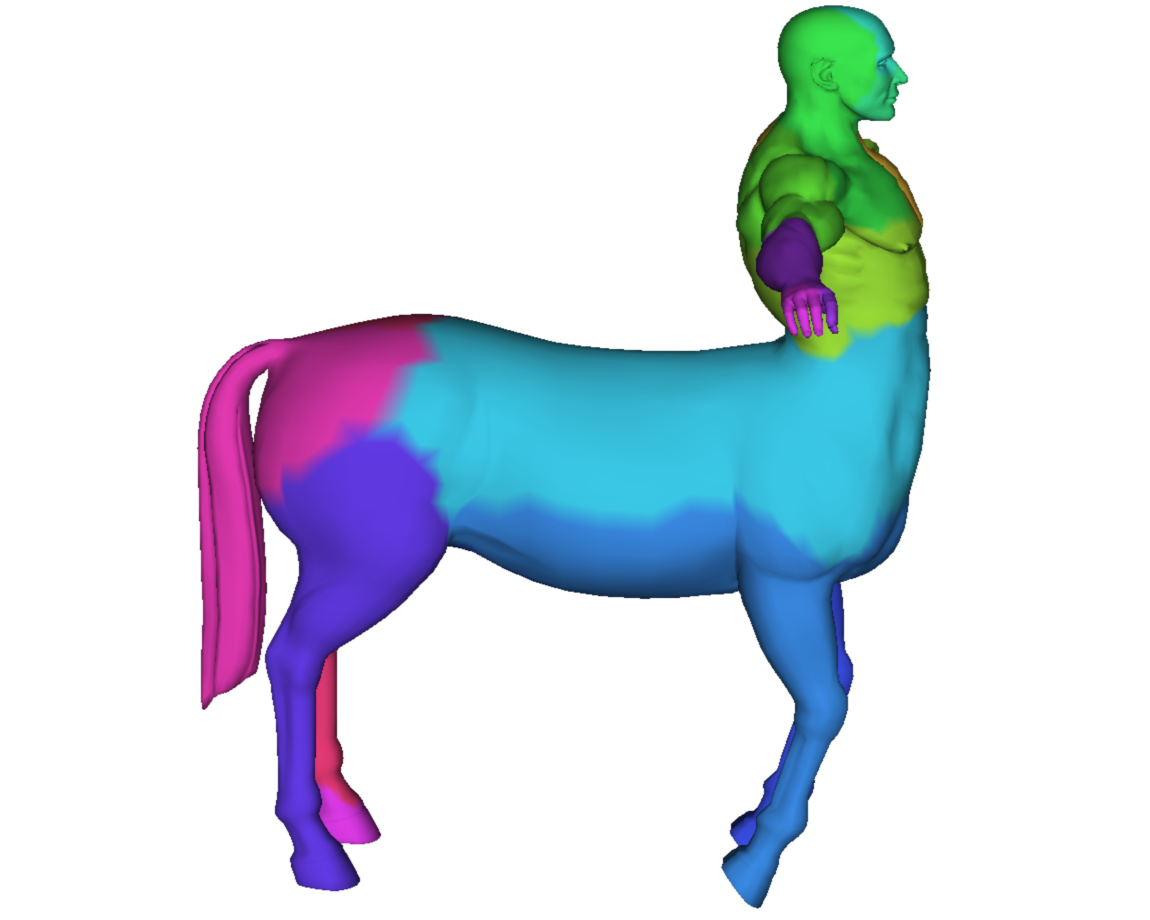
\includegraphics[width=\linewidth]{14}
        \caption{}
    \end{subfigure}
    ~
    \begin{subfigure}{0.4\linewidth}
        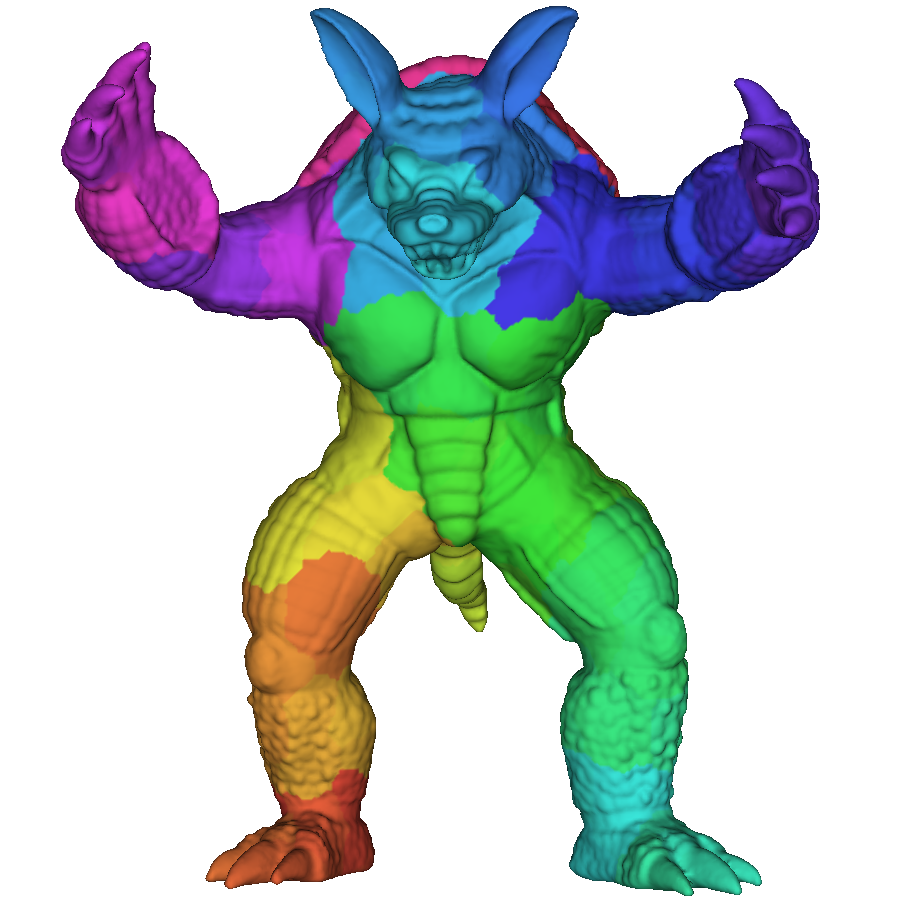
\includegraphics[width=\linewidth]{15}
        \caption{}
    \end{subfigure}
    \caption[Examples of Mesh partitioning.]
    {Models used in our experiments and their
     partitioning. (a) \emph{Cow}: 4,315 vertices. (b)
     \emph{Fandisk}: 6,475 vertices. (c) \emph{Centaur}: 15,768
     vertices. (d) \emph{Armadillo}: 172,974 vertices.}
    \label{fig:partitions}
\end{figure}

\begin{figure}
    \centering
    \begin{subfigure}{0.44\linewidth}
        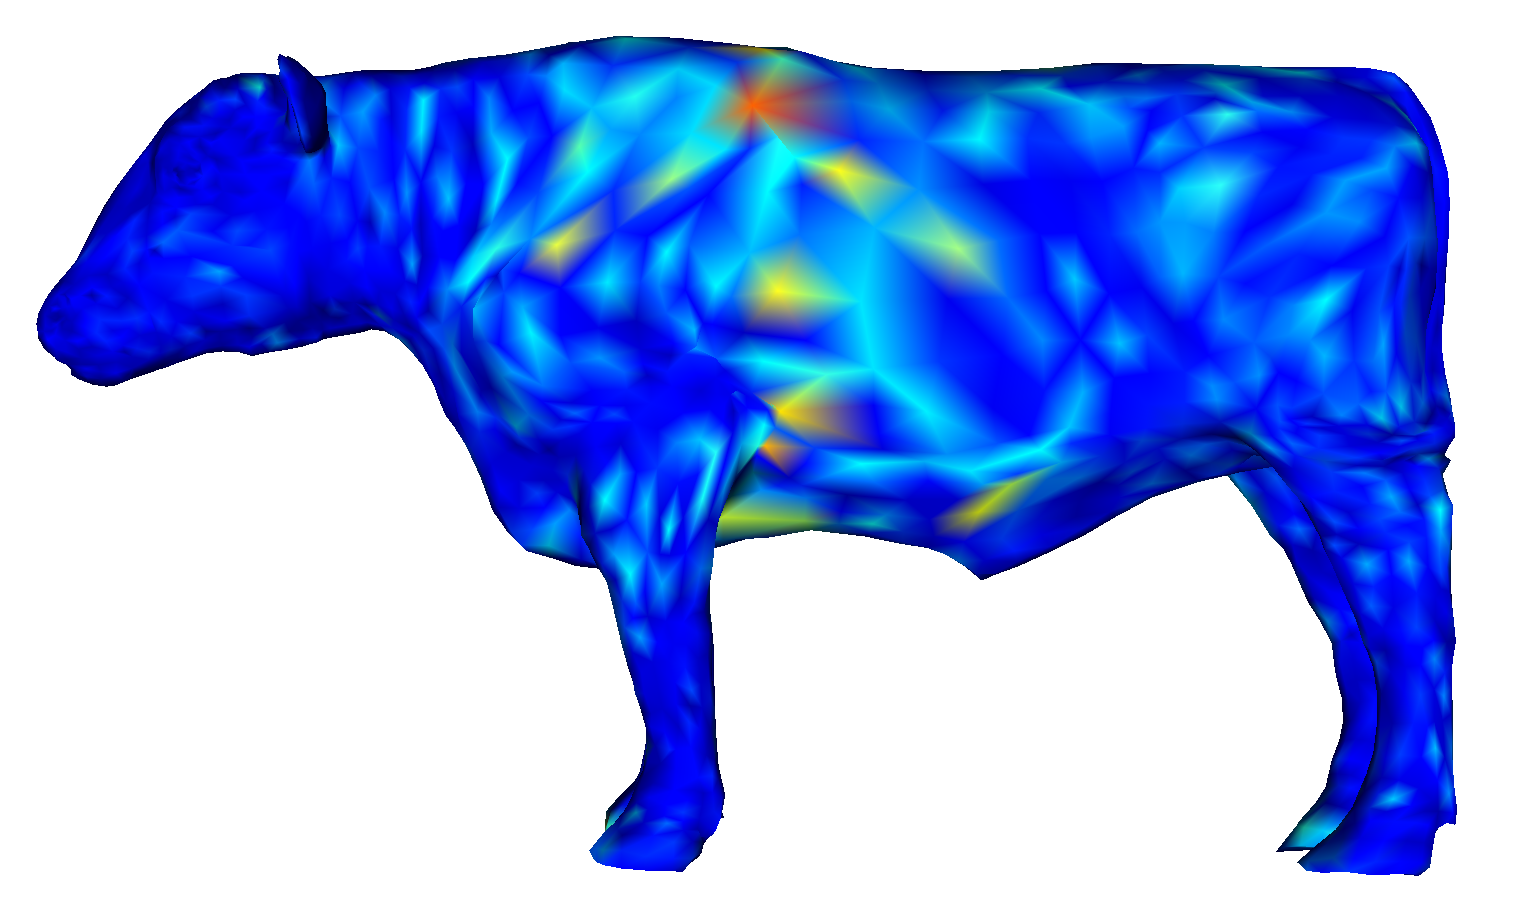
\includegraphics[width=\linewidth]{16}
        \caption{MHB, truncation}
    \end{subfigure}
    ~
    \begin{subfigure}{0.44\linewidth}
        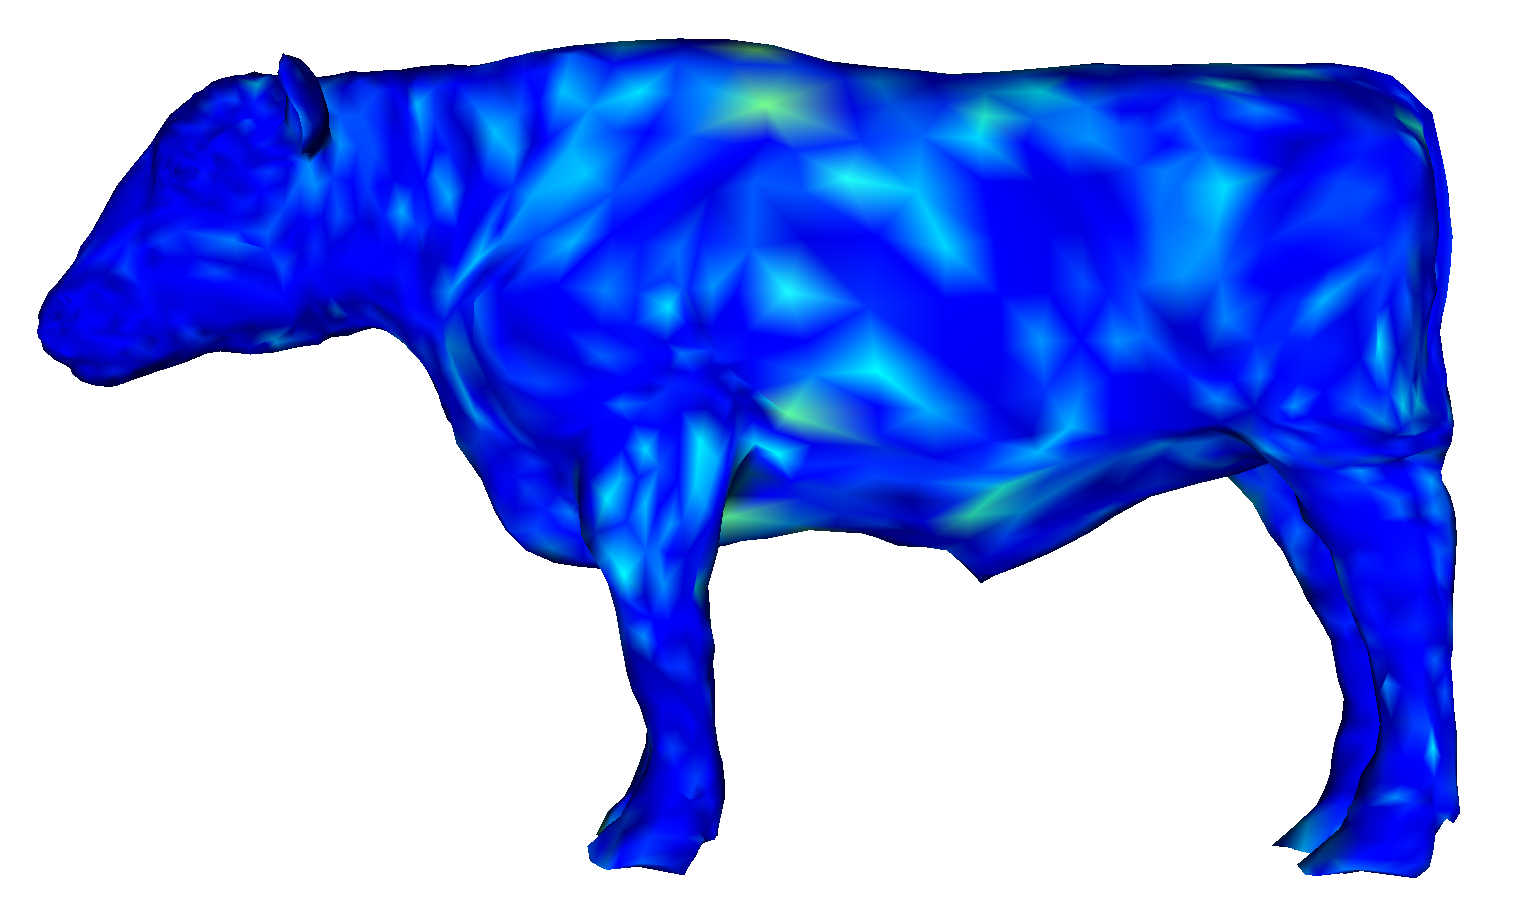
\includegraphics[width=\linewidth]{17}
        \caption{MHB, S-MP}
    \end{subfigure}
    \\
    \begin{subfigure}{0.44\linewidth}
        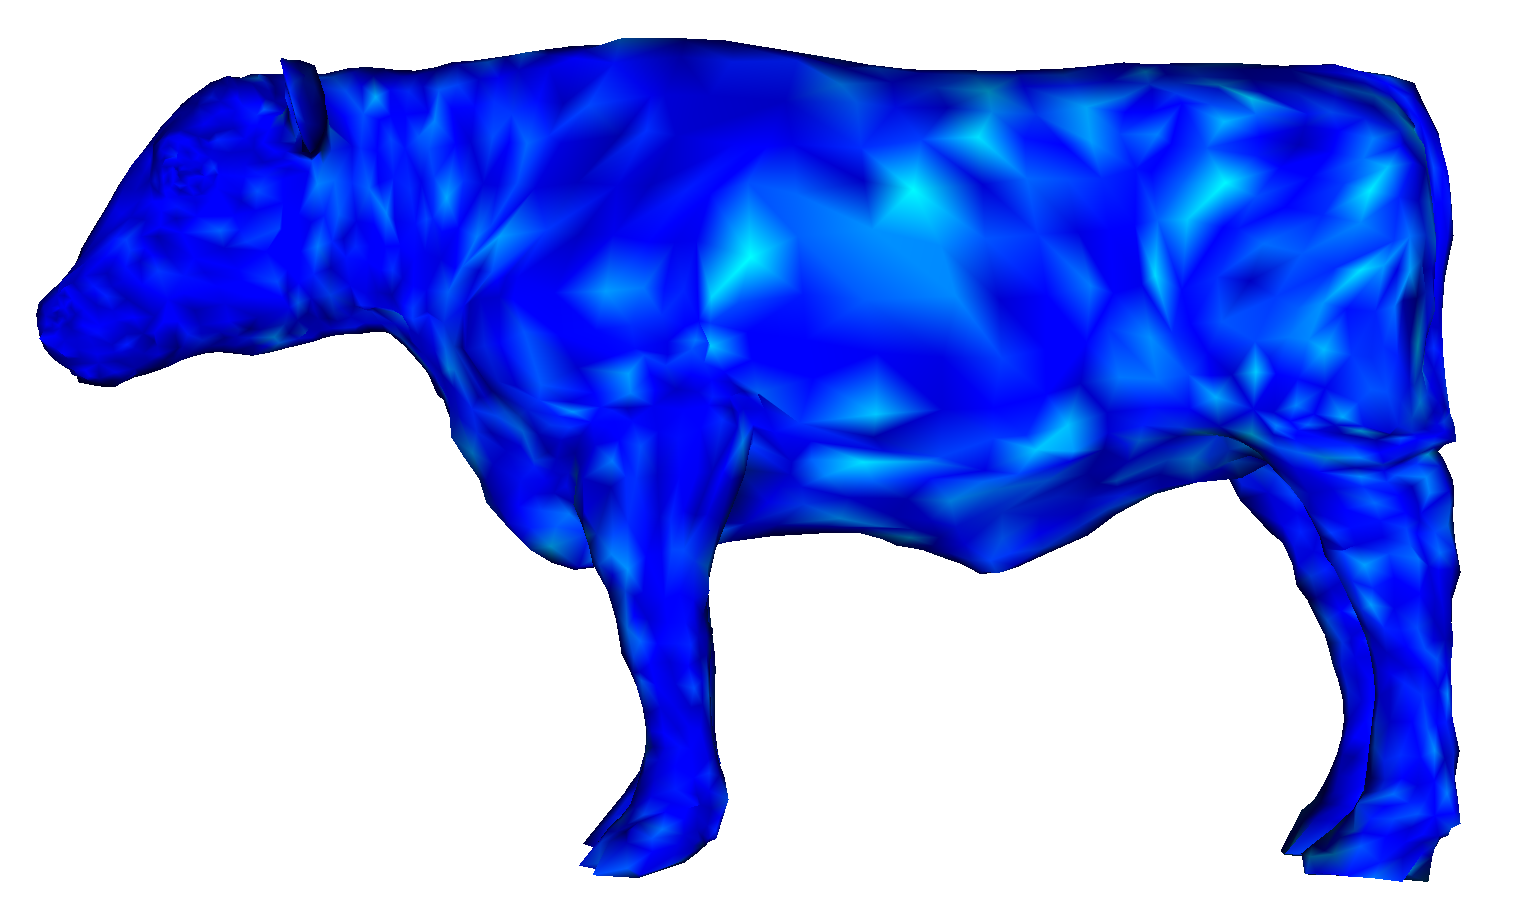
\includegraphics[width=\linewidth]{18}
        \caption{SGW, S-OMP}
    \end{subfigure}
    ~
    \begin{subfigure}{0.44\linewidth}
        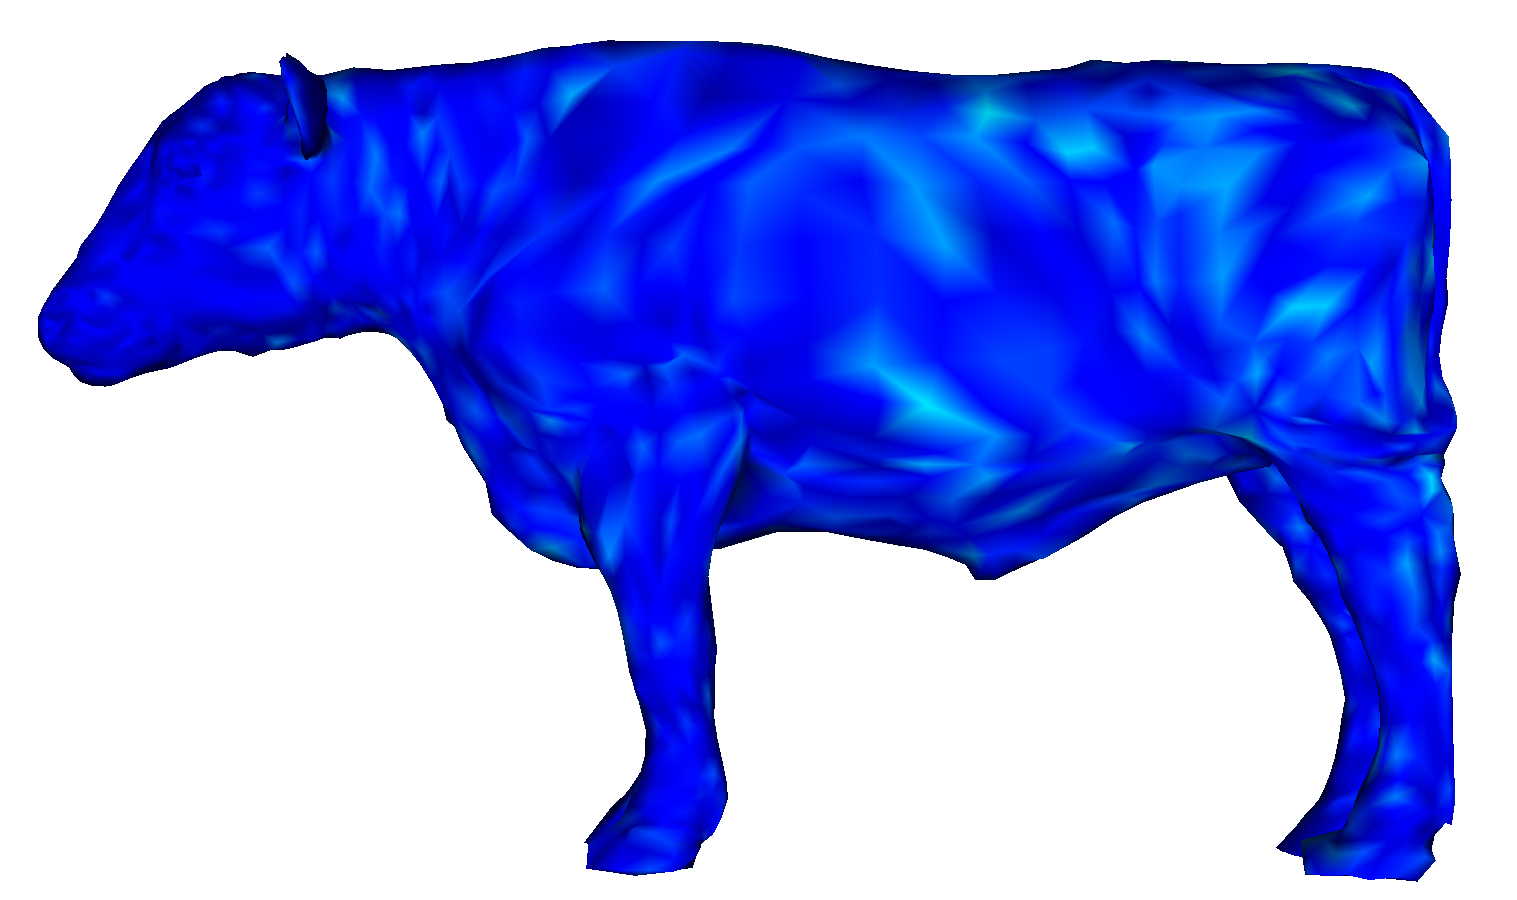
\includegraphics[width=\linewidth]{19}
        \caption{SGW+MHB, S-OMP}
    \end{subfigure}
    \\
    \begin{subfigure}{0.05\linewidth}
        (e)
    \end{subfigure}
    \begin{subfigure}{0.83\linewidth}
        \includegraphics[width=\linewidth]{20}
%        \caption{}
    \end{subfigure}
    \caption[Mesh compression performance on the cow model.]
    {Comparison of mesh compression performance
        for the cow model. (a-d) show the reconstructed meshes at 20\%
        compression ratio and visualize each vertex's positional error
        comparing with the original model. (e) shows how the
        compression errors change with the compression ratio.}
    \label{fig:coweval}
\end{figure}

\begin{figure}
    \centering
    \begin{subfigure}{0.45\linewidth}
        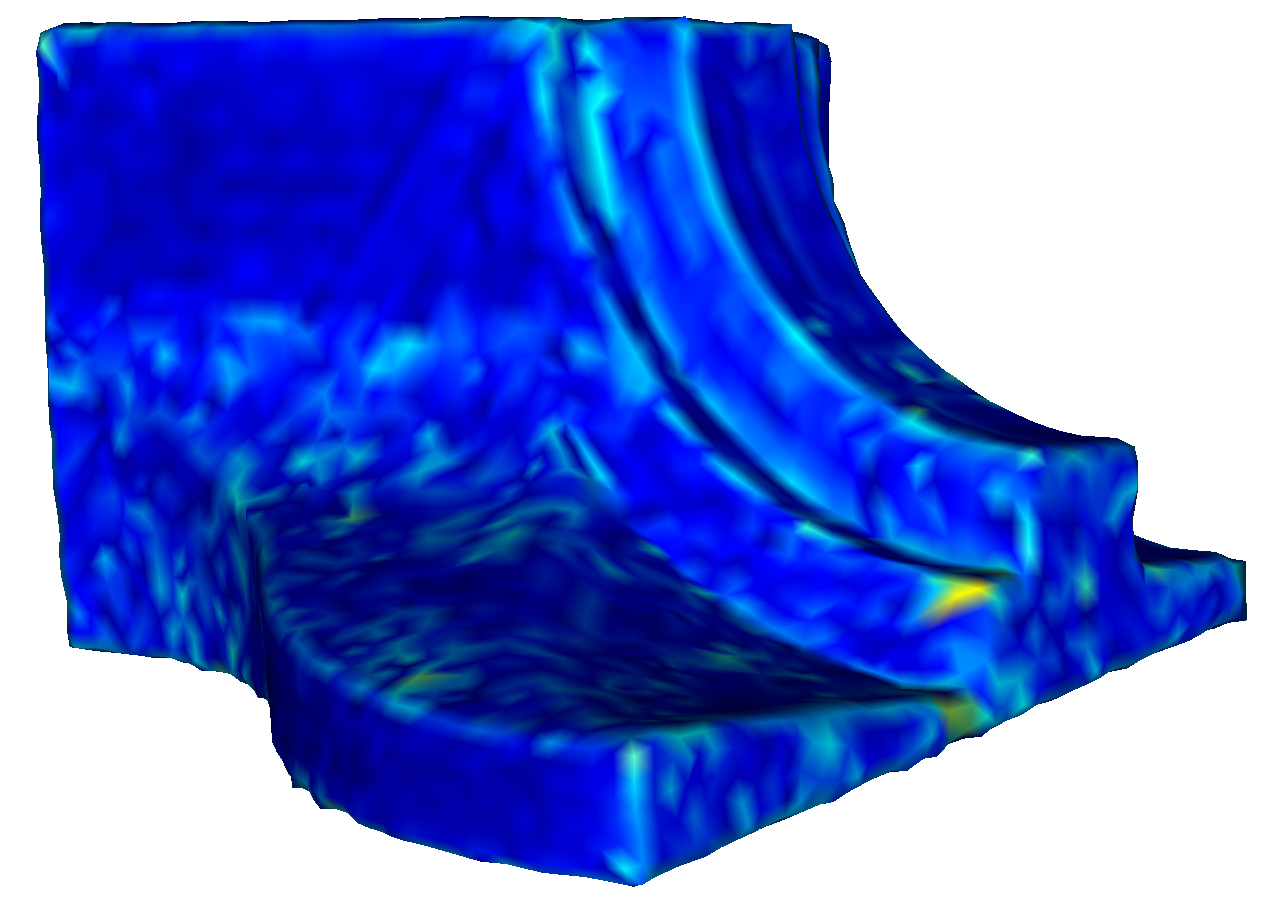
\includegraphics[width=\linewidth]{21}
        \caption{MHB, truncation}
    \end{subfigure}
    ~
    \begin{subfigure}{0.45\linewidth}
        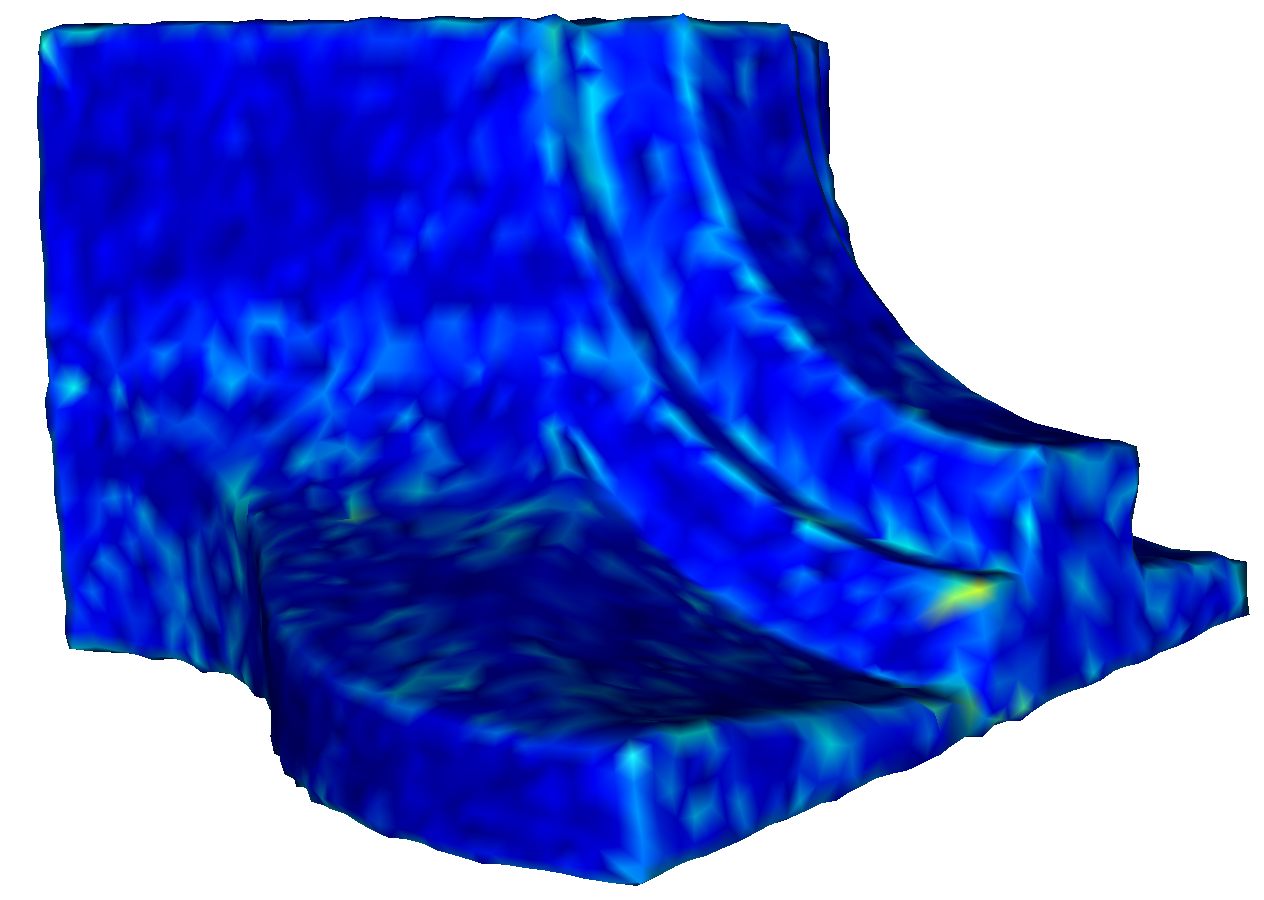
\includegraphics[width=\linewidth]{22}
        \caption{MHB, S-OMP}
    \end{subfigure}
    \\
    \begin{subfigure}{0.45\linewidth}
        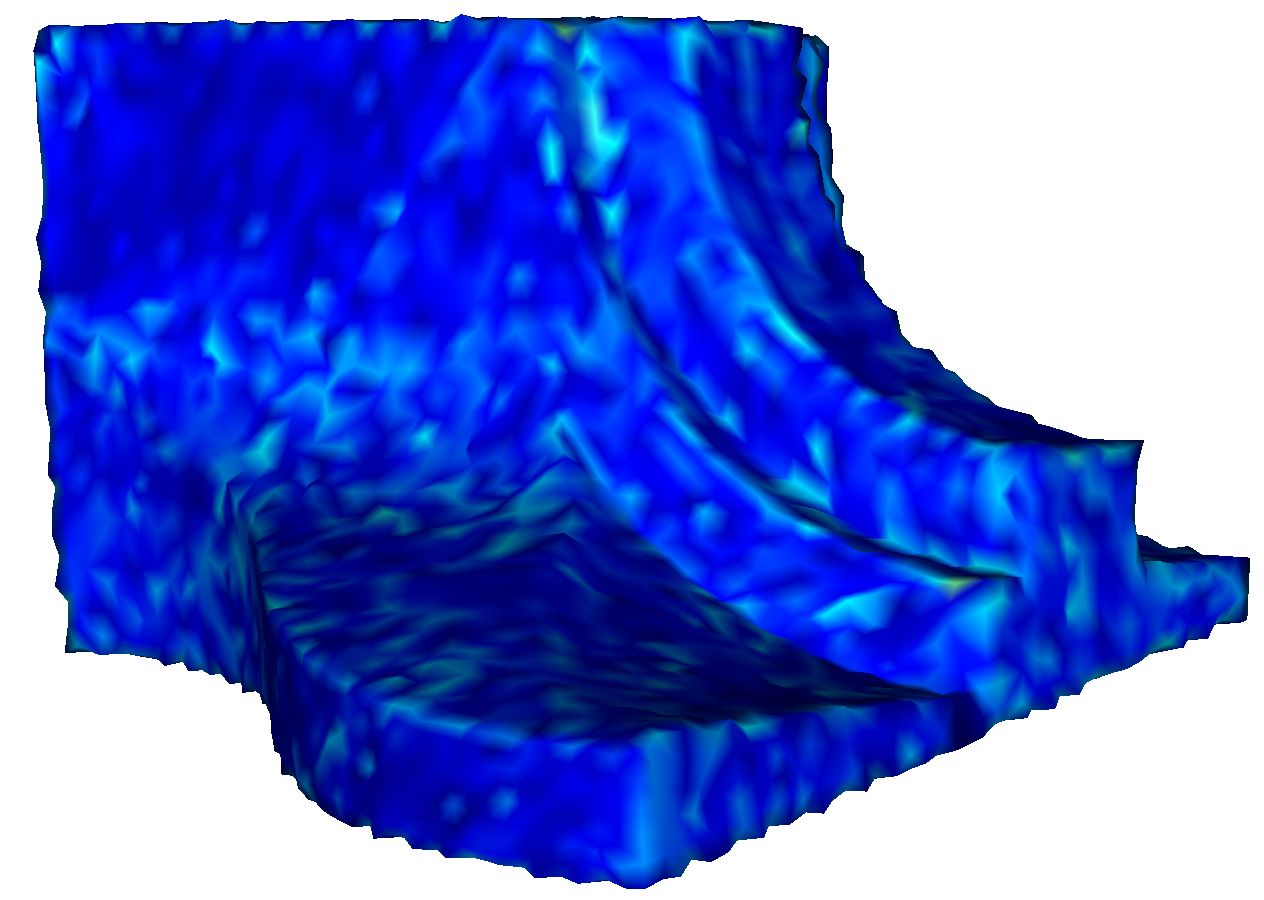
\includegraphics[width=\linewidth]{23}
        \caption{SGW, S-OMP}
    \end{subfigure}
    ~
    \begin{subfigure}{0.45\linewidth}
        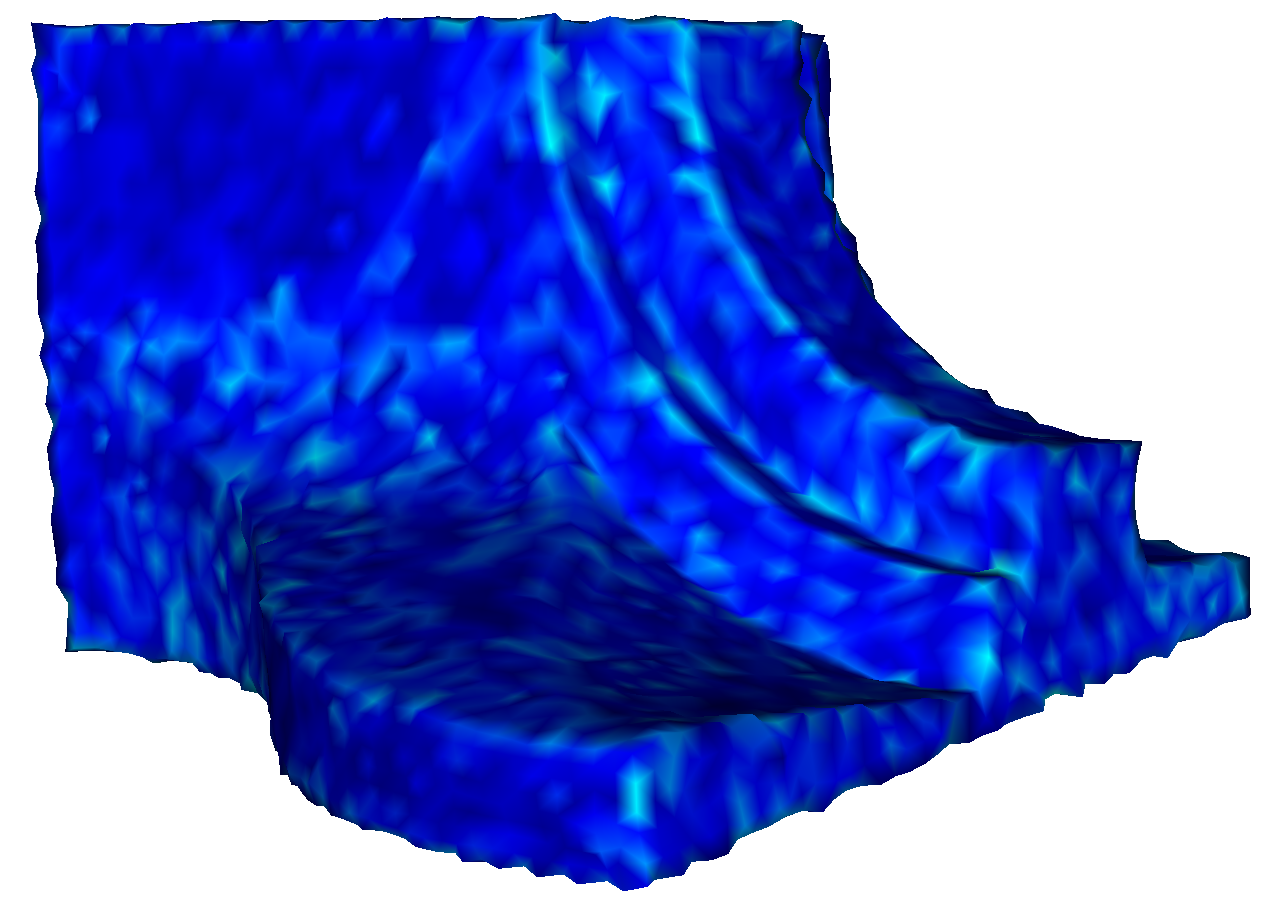
\includegraphics[width=\linewidth]{24}
        \caption{SGW+MHB, S-OMP}
    \end{subfigure}
    \\
    \begin{subfigure}{0.05\linewidth}
        (e)
    \end{subfigure}
    \begin{subfigure}{0.83\linewidth}
        \includegraphics[width=\linewidth]{25}
%        \caption{}
    \end{subfigure}
    \caption[Mesh compression performance on the fandisk model.]
    {Comparison of mesh compression performance
     for the fandisk model. (a-d) show the reconstructed meshes at
     20\% compression ratio and visualize each vertex's positional
     error comparing with the original model. (e) shows how the
     compression errors change with the compression ratio.}
    \label{fig:fandiskeval}
\end{figure}

\begin{figure}
    \centering
    \begin{subfigure}{0.45\linewidth}
        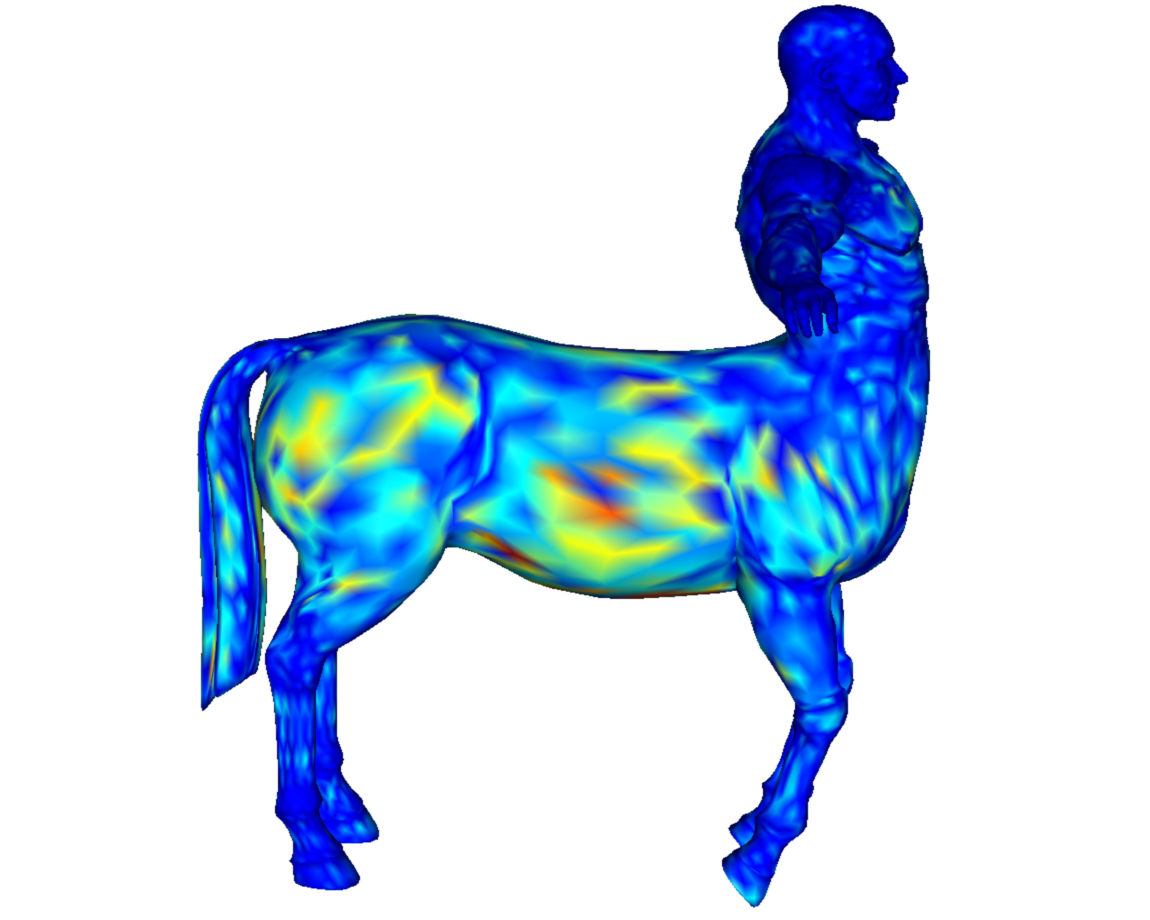
\includegraphics[width=\linewidth]{26}
        \caption{MHB, truncation}
    \end{subfigure}
    ~
    \begin{subfigure}{0.45\linewidth}
        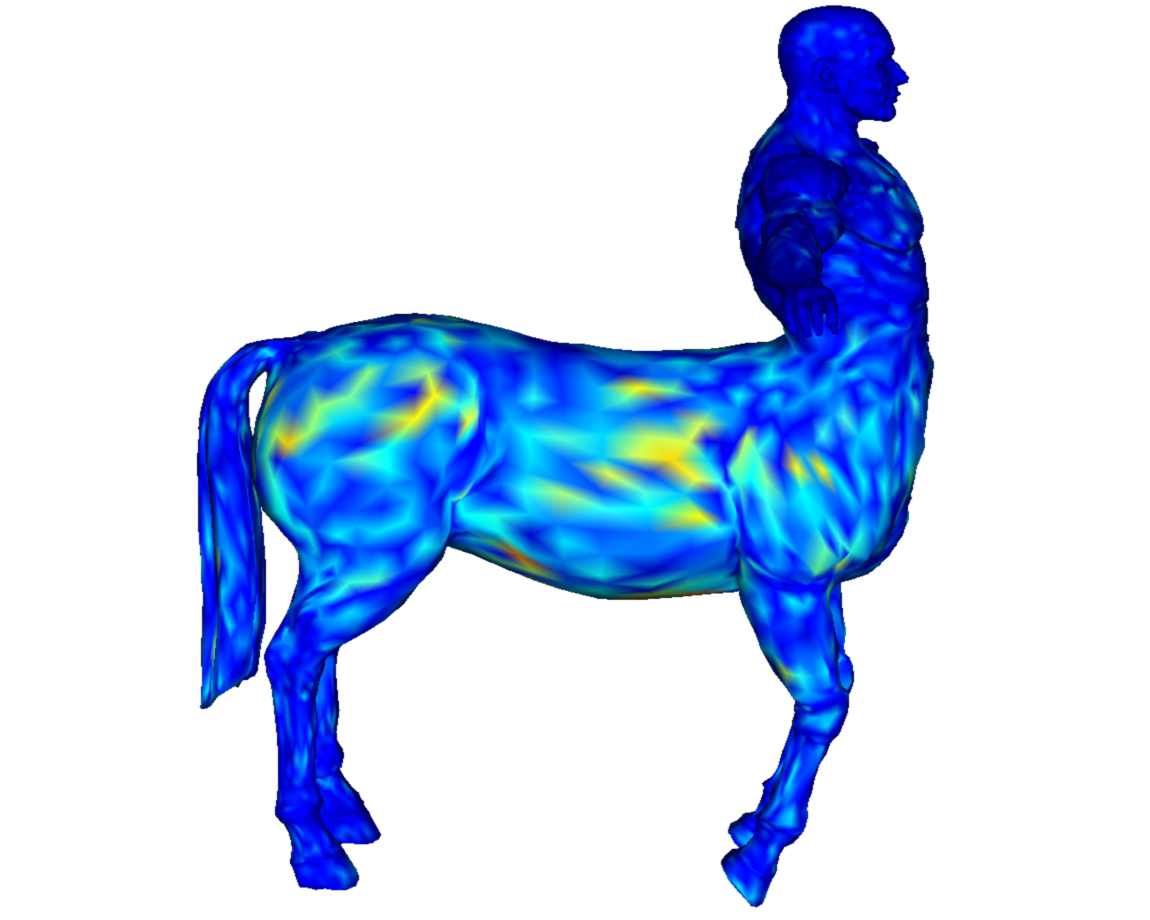
\includegraphics[width=\linewidth]{27}
        \caption{MHB, S-OMP}
    \end{subfigure}
    \\
    \begin{subfigure}{0.45\linewidth}
        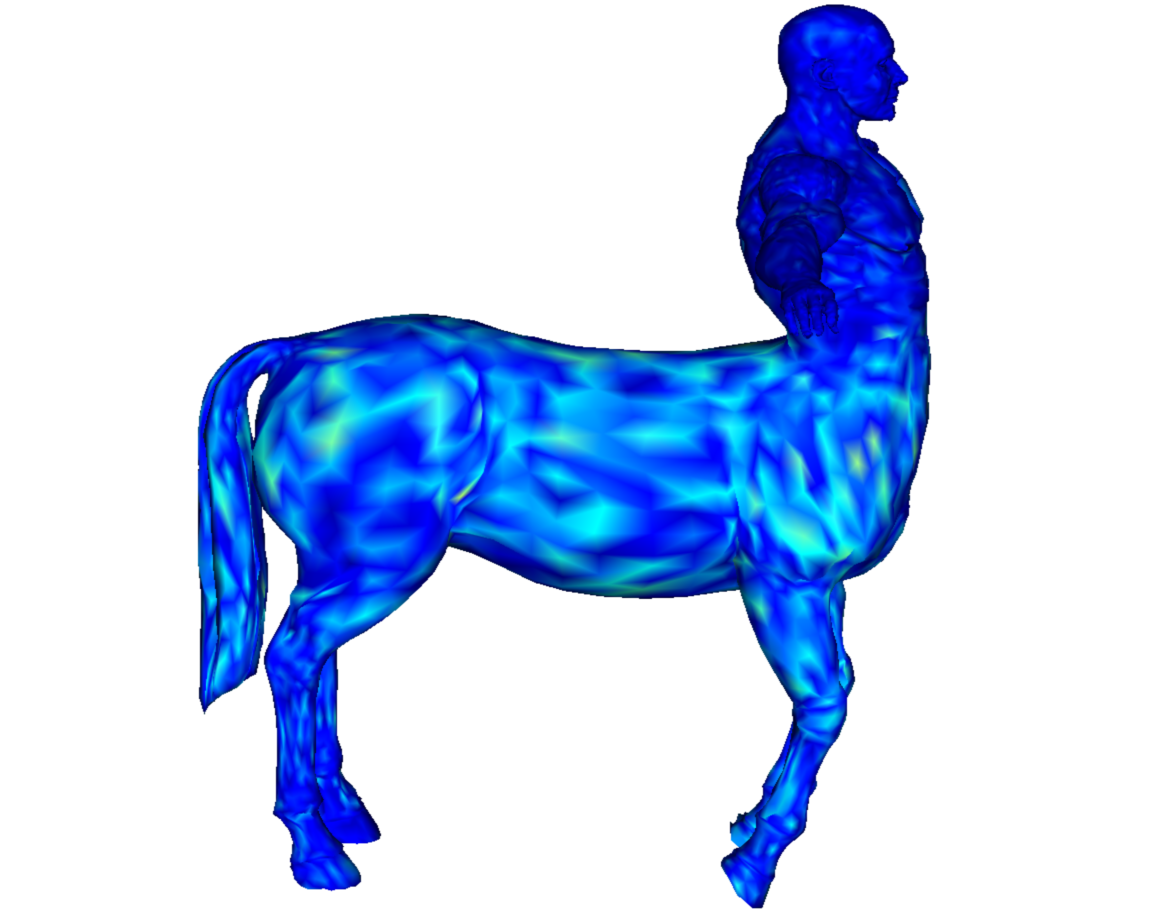
\includegraphics[width=\linewidth]{28}
        \caption{SGW, S-OMP}
    \end{subfigure}
    ~
    \begin{subfigure}{0.45\linewidth}
        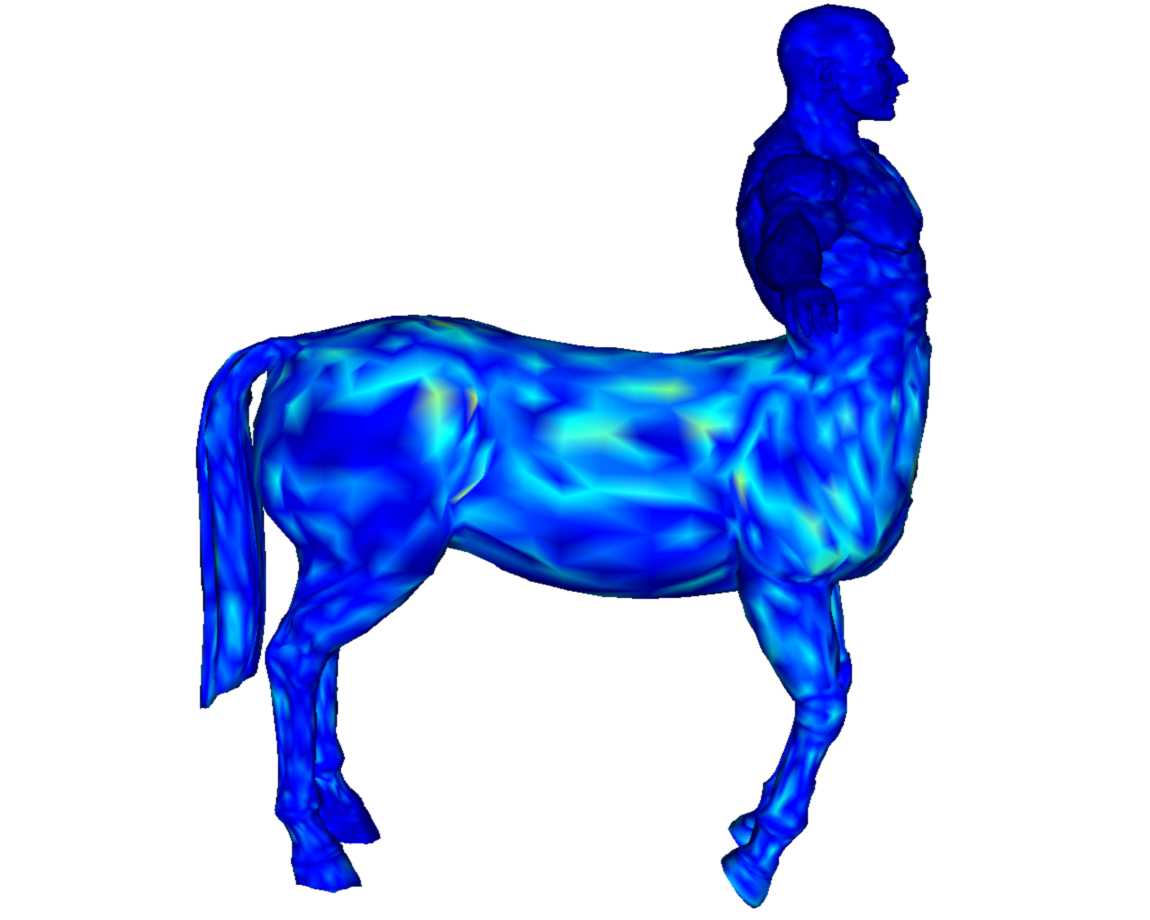
\includegraphics[width=\linewidth]{29}
        \caption{SGW+MHB, S-OMP}
    \end{subfigure}
    \\
    \begin{subfigure}{0.05\linewidth}
        (e)
    \end{subfigure}
    \begin{subfigure}{0.83\linewidth}
        \includegraphics[width=\linewidth]{30}
%        \caption{}
    \end{subfigure}
    \caption[Mesh compression performance on the centaur model.]
    {Comparison of mesh compression performance
     for the centaur model. (a-d) show the reconstructed meshes at
     20\% compression ratio and visualize each vertex's positional
     error comparing with the original model. (e) shows how the
     compression errors change with the compression ratio.}
    \label{fig:centaureval}
\end{figure}

\begin{figure}
    \centering
    \begin{subfigure}{0.44\linewidth}
        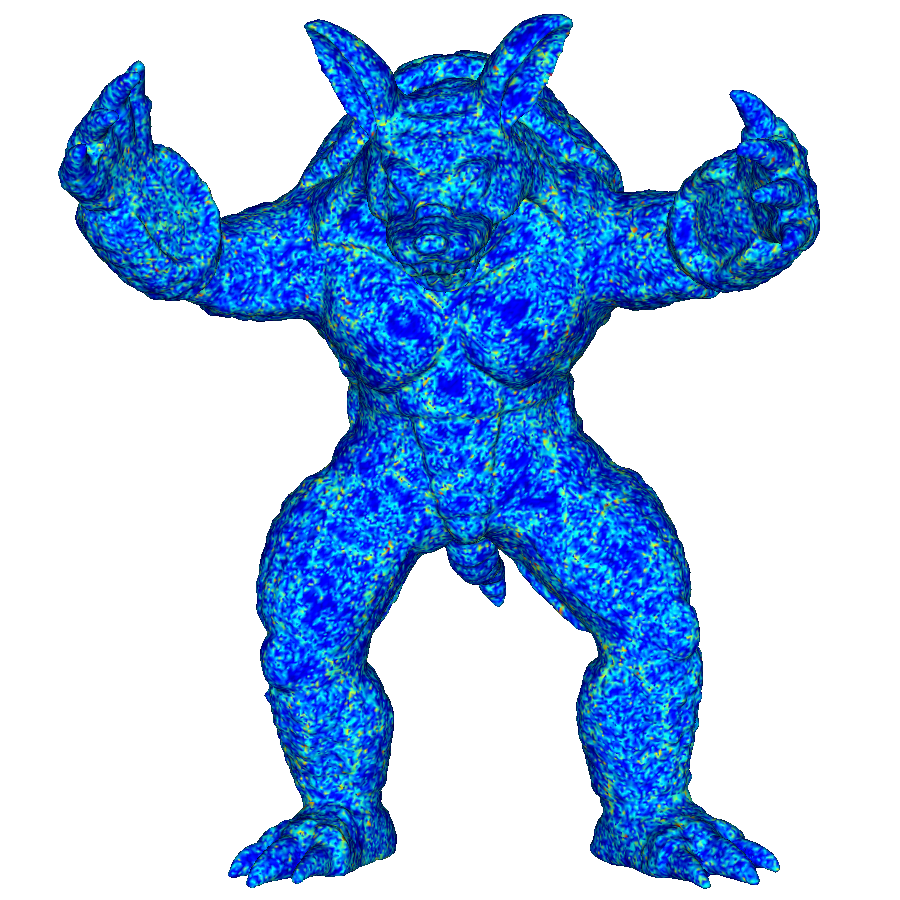
\includegraphics[width=\linewidth]{31}
        \caption{MHB, truncation}
    \end{subfigure}
    ~
    \begin{subfigure}{0.44\linewidth}
        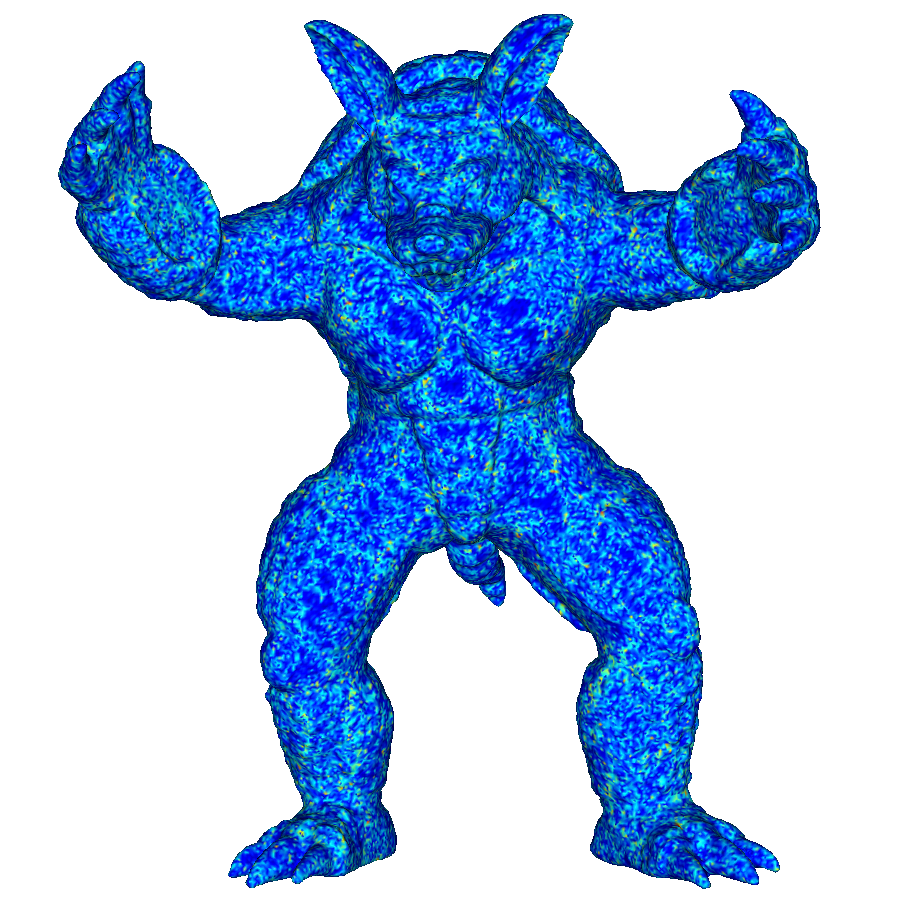
\includegraphics[width=\linewidth]{32}
        \caption{MHB, S-MP}
    \end{subfigure}
    \\
    \begin{subfigure}{0.44\linewidth}
        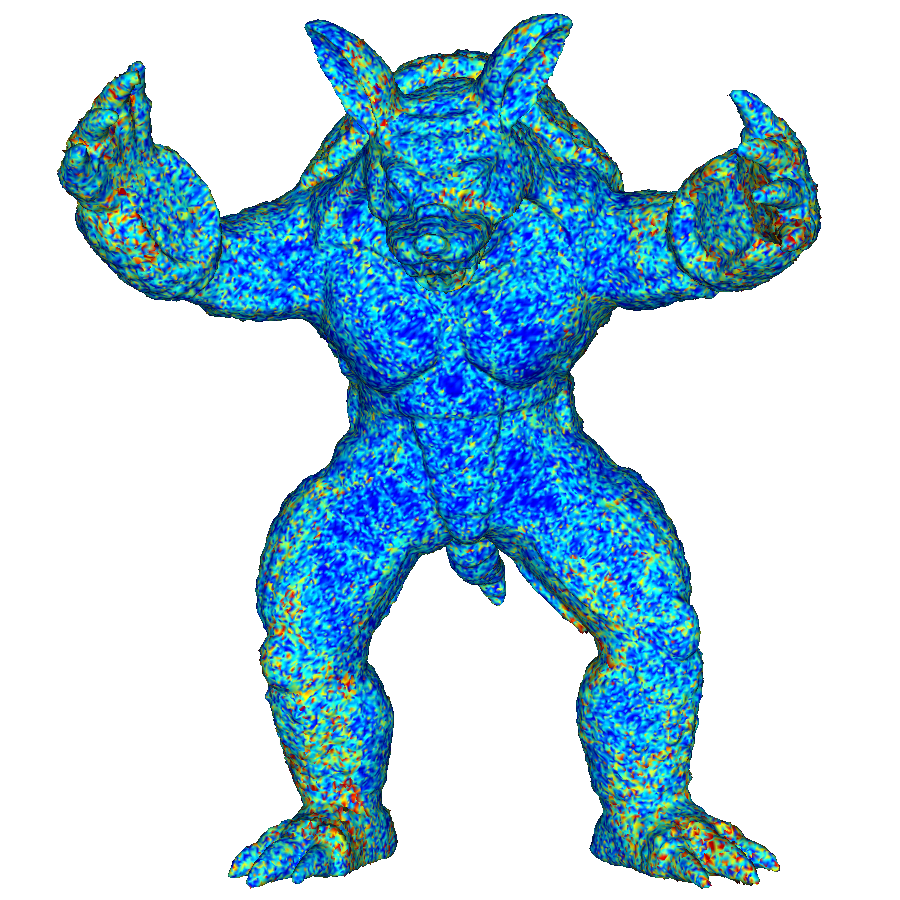
\includegraphics[width=\linewidth]{33}
        \caption{SGW, S-OMP}
    \end{subfigure}
    ~
    \begin{subfigure}{0.44\linewidth}
        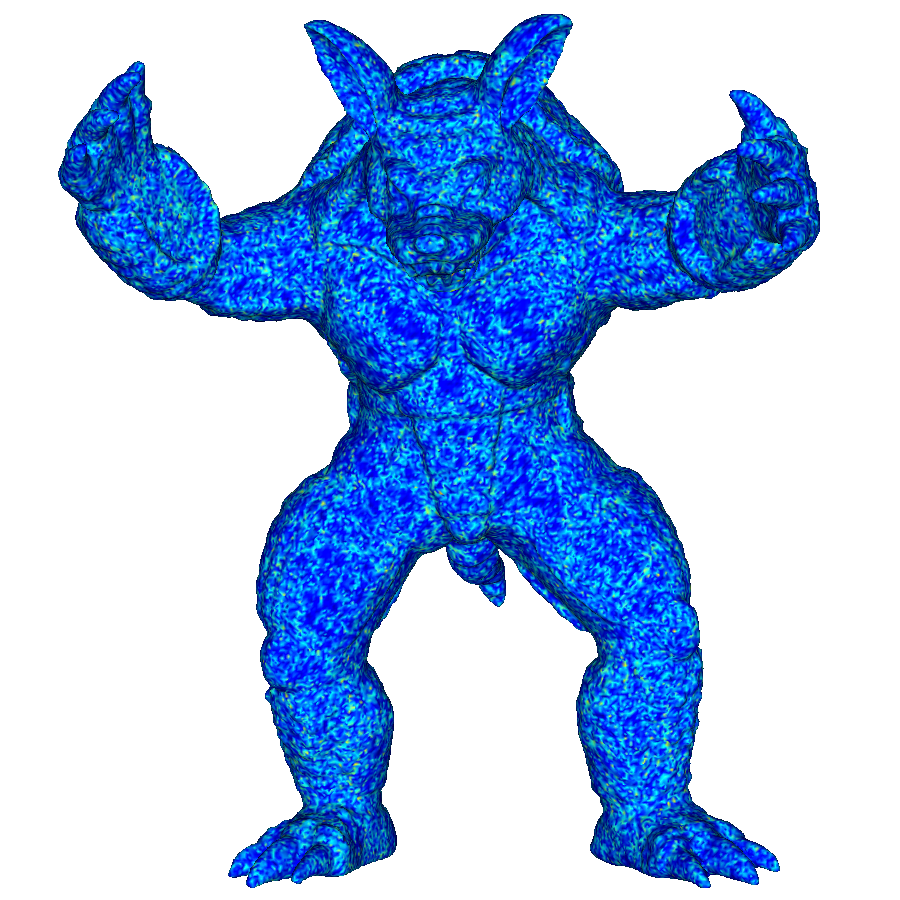
\includegraphics[width=\linewidth]{34}
        \caption{SGW+MHB, S-OMP}
    \end{subfigure}
    \\
    \begin{subfigure}{0.05\linewidth}
        (e)
    \end{subfigure}
    \begin{subfigure}{0.83\linewidth}
        \includegraphics[width=\linewidth]{35}
        %\caption{}
    \end{subfigure}
    \caption[Mesh compression performance on the armadillo model.]
    {Comparison of mesh compression performance
        for the armadillo model. (a-d) show the reconstructed meshes
        at 15\% compression ratio and visualize each vertex's
        positional error. Comparing (c) and (d), it is obvious that the SGW+MHB dictionary
        produces much smaller positional error than the SGW-only dictionary.
        (e) shows how the compression errors change with the compression
        ratio.}
    \label{fig:armadilloeval}
\end{figure}

In all our tests, we compare the compression performance between the
classical spectral compression method based on MHB coefficient
truncation \cite{Karni2000} and our sparse approximation
compression method employing three different dictionaries: (1) S-MP
with the MHB-only dictionary; (2) S-OMP with the SGW-only dictionary;
(3) S-OMP with the SGW+MHB dictionary.

\begin{table}[th] 
\centering
\begin{tabular}{ |c|c|c|c|c| }
\hline
Model (\#vertices) & Ratio & Error & Error Decrease & Timing (s) \\ 
\hline
\multirow{2}{*}{Cow (4,315)} & 20\% & 1.91e-3 & 18.0\% & 3.4 \\
                             & 40\% & 1.12e-3 & 27.5\% & 10.5 \\
\hline
\multirow{2}{*}{Fandisk (6,475)} & 20\% & 1.09e-3 & 11.6\% & 7.2 \\
                                 & 40\% & 5.74e-4 & 28.1\% & 18.9 \\
\hline
\multirow{2}{*}{Centaur (15,768)} & 20\% & 1.03e-3 & 20.3\% & 19.6 \\
                                  & 40\% & 5.89e-3 & 37.7\% & 50.3 \\
\hline
\multirow{2}{*}{Armadillo (172,974)} & 20\% & 2.26e-3 & 9.4\% & 178.0 \\
                                     & 40\% & 1.76e-3 & 15.7\% & 354.5 \\
\hline
\end{tabular}
\caption[Statistics of compression errors and running times using different dictionary.]
{Statistics of compression errors and
    running times using the S-OMP algorithm with SGW+MHB dictionary
    (on a machine with quad-core 2.4GHz processor and 16G RAM).
    The ``Error Decrease'' column shows the decrease of compression
    error compared with the MHB truncation method.}
\label{tab:stat}
\end{table}

Fig.~\ref{fig:partitions} shows the original meshes and their
partitioning used in our experiments, including a ``cow'', a
``fandisk'', a ``centaur'', and a ``armadillo'' model. All meshes are
scaled to have unit surface area. The evaluation results are shown in
Fig.~\ref{fig:coweval}, Fig.~\ref{fig:fandiskeval},
Fig.~\ref{fig:centaureval}, and Fig.~\ref{fig:armadilloeval},
respectively. For each 3D mesh, we compute the approximation at
specified compression ratios in the ranges between 5\% and 80\%. The
overall compression quality is measured by the combined geometric and
differential error (see Eq.~(\ref{eq:metric})) w.r.t. the original
mesh. Table~\ref{tab:stat} documents the compression errors and timing
of S-OMP with SGW+MHB dictionaries, and compares the errors with the
MHB coefficient truncation method.

From the experimental results, we see that, with a properly chosen
dictionary, simultaneous sparse approximation can generate
higher-fidelity mesh compression than the MHB truncation method at the
same compression ratio. The SGW functions are a viable choice for
efficient mesh approximation, but the performance of a SGW-only
dictionary degenerates significantly when the required compression
ratio is small or the mesh is large, which is especially evident in the armadillo
model (Fig.~\ref{fig:armadilloeval}). A dictionary combining SGW and MHB
overcomes this deficiency, and its performance in mesh approximation
is consistently superior to the MHB truncation method.

\section{Chapter Summary}

In this chapter, we have developed an algorithm for sparse approximation
of 3D shapes. We employed the spectral graph wavelets (SGW) to
construct the redundant dictionary of shape bases, and used
simultaneous orthogonal matching pursuit to seek a sparse
representation of the input mesh. The use of spatially-localized
wavelets makes our algorithm very suitable and powerful for better
approximating shapes with many local and fine geometric features.
Through comprehensive experiments we have demonstrated the superiority
of our algorithm for approximating complex 3D objects at different
compression ratio settings towards sparse representation.

As for the future work, we plan to investigate other
improved formulations of graph wavelets as basis vectors to enhance
the expressive power of dictionary. For example, it is more desirable
to have data-specific, anisotropic wavelets that are adaptive to shape
features such as sharp corners and edges, which can further facilitate
more efficient and sparse representation of shape geometry. We also
plan to explore faster sparse approximation algorithms such as
stagewise orthogonal matching pursuit (StOMP)~\cite{Donoho2012} to
arrive at better time performance. 
\graphicspath{{fig-inpainting/}}
\chapter{Surface Inpainting}
\label{chap:inpainting}

\section{Introduction}
In principle, surface inpainting refers to the completion or recovery of
missing shape geometry based on the shape information that is currently
available. The most prominent application of surface inpainting is mesh repair.
Due to factors such as occlusions, low reflectance, and quality limitations of
scanning equipments, 3D models generated from range scanners often contain
holes that need to be filled; sometimes the source model itself has missing
pieces and requires digital repair to attain a complete model. Another common
application of surface inpainting is to remove geometric features because of
shape editing needs. This is achieved by replacing the unwanted shape regions
with inpainting patches.

From the statistical point of view, surface inpainting can be viewed as an
estimation problem which infers the missing geometry from the observable shape,
and the inpainting result is determined by the statistical model we have
adopted. Generally speaking, there is no universally acceptable ``correct''
estimation; selecting the best inpainting is usually subjective or dependent on
the requirement of downstream applications.

Most existing surface inpainting methods tackle the problem only in
the mesh domain. These methods typically employ some geometric
constraints as heuristics to ensure that the obtained inpainting patch
is visually pleasing and blend naturally with its neighboring
geometry. The primary issue of geometry-constrained inpainting is that
these methods only utilize the shape information in the vicinity of
missing regions rather than consider the model in question in its
entirety.

Our new surface inpainting method documented is inspired
by the theory of sparse signal recovery and compressed sensing. The
intuition is that for a meaningful 3D model, even though its global
geometry is a high-dimensional signal, it most likely has a
low-dimensional intrinsic structure. That is to say, the
high-dimensional shape signal actually lives in a low-dimensional
subspace, which can be captured by a sparse coefficient representation
in some transformed (e.g., Fourier) domains. In another word, the
coordinate function of a shape with $N$ vertices can be decomposed as or
well approximated by the linear combination of $k\ll N$ basis signals.
According to the compressed sensing theory, the sparse coefficient
representation can be recovered from partial measurements as long as
the signal is sufficiently sparse and the sensing matrix satisfies
certain properties~\cite{Candes2006}.

The critical idea of our new inpainting algorithm is to estimate the
spectral coefficient representation of the shape geometry from partial
observations by imposing sparsity constraints on the reconstructed
coefficients, exploiting the fact that most 3D models are highly
compressible with respect to their Laplacian eigenfunctions~\cite{Karni2000}.
To the best of our knowledge, the utility of Laplacian eigenbasis towards
the shape inpainting application has not yet been explored in the past.
The estimation problem can be formulated with a data term strongly emphasizing
fidelity to the observations and a penalty term constraining sparsity of the
representation. Thus, the surface inpainting could be transformed to a
sparse signal recovery problem and can be solved by either $l_0$ or
$l_1$ optimization techniques. Such effort represents our first
attempt towards technical innovation.

The primary advantage of our method is that the inpainting takes into
account the information of all the remaining shape instead of only the
vicinity of missing regions. Rather than directly estimating the
missing geometry, we actually estimate the reconstruction coefficients
of the whole original shape. Since the mesh Laplacian basis functions are
smooth and have global support, the reconstructed inpainting shape is
naturally smooth and globally coherent with a simple intrinsic
structure.

The main contributions of this work are:
\begin{itemize}

\item We introduce a new surface inpainting framework based on
  representations in the transformed domain and sparsity constraints
  on reconstruction coefficients. This framework can make use of the
  information of the whole remaining shape and inpainting results
  tend to be simple and globally coherent.

\item We study the sparsity of 3D shapes with respect to their
  Laplacian eigenbases and show their effectiveness in surface
  inpainting.

\item We demonstrate the high performance of our inpainting method
  with several examples in hole filling and mesh editing.

\end{itemize}


\section{Related Work}
\label{sec:related}

\subsection{Surface Inpainting}

Many methods have been proposed in the research literature dealing
with the general problem of surface inpainting, bearing different
names such as hole filling, mesh completion, and surface restoration.
We refer readers to~\cite{Attene2013} for a recent survey of popular
algorithms for hole filling and mesh completion.

One simple approach for surface inpainting is by filling the missing region
with an inpainting patch that interpolates the surrounding geometry. The
interpolating patch may be generated with simple polynomial
functions~\cite{Wang2007}, triangular B-splines~\cite{Pfeifle1996}, or radial
basis functions~\cite{Branch2006}, and are generally smooth and continuous
across the boundaries. The interpolation-based approaches, however, only work
well with disk-like holes and are not suitable for filling regions with
complex boundaries.

Typical mesh-based hole filling algorithms have two steps: (1) Find an
initial triangulation of the missing region defined by the hole
boundary; (2) Optimize the inserted mesh to improve its fairness and
coherence with surrounding shapes. In \cite{Liepa2003}, Liepa
performed hole triangulation with a dynamic programming technique
taking into account the dihedral angles and areas of the created
triangles. The inserted mesh is then optimized with Laplacian
smoothing to improve fairness. In \cite{Zhao2007}, surface holes are
patched by an advancing-front mesh generation method, and the vertex
positions are optimized by solving a Poisson equation based on the
desirable triangle normals computed from boundary vertices. In \cite{Bac2008},
the coordinates of the inserted vertices are optimized by minimizing the
discrete thin-plate energy.
In \cite{Li2010}, \cite{Wang2012} and \cite{Ngo2013}, complex holes are
first partitioned into sub-holes by feature curves extended from the
existing parts; typical hole-filling then can be performed on these
sub-holes which are much more planar.

Another class of inpainting algorithms are based on variational
methods. The basic idea is to iteratively evolve the inpainting shape
by optimizing a functional that constrains certain geometric
properties of the inserted mesh, e.g., positions, areas, tangency, and
curvatures. In \cite{Pernot2006}, Pernot et al. developed a hole
filling algorithm which minimizes the variational involving curvature
between the surrounding and inpainted geometry. In
\cite{Caselles2008}, the completing surface is chosen such that a
power of the mean curvature is minimized. In \cite{Clarenz2004},
Clarenz et al. proposed a shape restoration algorithm by computing the
$l_2$-gradient flow of the Willmore energy which ensures the
continuity of the normal field.

Finally, a large number of mesh inpainting methods can be classified as
exemplar-based or template-based. The basic idea is to find a known patch or a
template model that has similar context with the damaged or missing region and then
adapt the selected patch for inpainting. Symmetry-guided methods
\cite{PaulyMitraWallnerEtAl2008, Sharf2004, Park2005, LiYinWeiEtAl2011}
take advantage of intrinsic shape symmetry to repair damaged regions by
transplanting similar regions from the object itself; the pitfall is that it
only works when the damaged region's corresponding symmetric counterpart exists
and is not missing or damaged. Template-guided methods \cite{Kraevoy2005, GalShamirHassnerEtAl2007, ZhangYuManheinEtAl2015, WeiYuLiEtAl2011,Pauly2005}
conduct mesh completion by matching the incomplete region with a template model
which may be deformed to adapt to the context. The main challenges are:
(1) Suitable template model may not be available in the template database;
(2) Inpainting results can be affected by cross-shape parameterization.

\subsection{Sparse Signal Recovery and Inpainting}

Recent years have witnessed a surge in the research of sparsity-based
signal recovery. The fundamental idea is that a sufficiently sparse
signal can be reliably reconstructed from partial measurements by
exploiting the sparsity cue.

Sparse signal recovery has seen most success in compressed sensing
applications, where the measurement/sensing matrix is typically chosen
as a normalized random matrix which satisfies the restricted isometry
property with high probability. For the inpainting problem, the
measurement is expressed as a mask matrix, which is not strictly a
valid compressed sensing process. Nonetheless, we can still take
advantage of the sparsity constraints to recover the original signals
in many situations.

For image inpainting and restoration tasks, many algorithms based on
 sparse representation have been published. In \cite{Guleryuz2006} and
\cite{Guleryuz2006a}, Guleryuz proposed an algorithm for image
recovery based on adaptive sparse representation. In \cite{Elad2005},
images are decomposed into texture and cartoon components, each of
which is sparse with respect to a particular dictionary; the missing
parts then can be easily reconstructed. In \cite{Fadili2005} and
\cite{Fadili2009}, Fadili et al. formulated image inpainting as a
maximum-likelihood estimation problem with a sparsity-promoting prior
penalty imposed on the reconstructed coefficients. A similar
formulation is proposed in \cite{Cai2008} where images have sparse
framelet representations and the incomplete image can be restored via
an iterative shrinkage algorithm. This formulation balances the
sparsity of coefficients, fidelity to the existing data, as well as
the smoothness of the solution. In \cite{Ogawa2011}, Ogawa et al.
proposed an image recovery algorithm based on sparse representation,
in which the low-dimensional subspaces optimal for targeted missing
textures are adaptively selected.

There have been very few works on the sparsity-induced recovery of
signals defined on graphs. In \cite{Zhu2012}, Zhu
and Rabbat proposed to use the dictionary of graph Laplacian
eigenfunctions to recover smooth and sparse graph signals and applied them
to the reconstruction of wireless sensor networks data from partial
node readings. To the best of our knowledge, our method is the first
of such attempts to tackle the problem of geometry
inpainting/completion via sparse signal recovery.

\section{Variational Inpainting Model}
\label{sec:inpaint:model}

The problem of mesh signal inpainting can be stated as follows.
Consider a triangle mesh $M=\{V,E\}$ with $n$ vertices, where $V$ and
$E$ denote the set of vertices and edges, respectively. Let
$\mathbf{f}\in\mathbb{R}^n$ be a vector signal defined on the mesh
vertices. Assume the signal values at a subset of vertices $V'\subset
V$ are already known, the goal of inpainting is to compute a
reasonable estimate of the remaining signal values at $V - V'$. For
the problem of inpainting surface geometry, the mesh signal is the
coordinate function and the unknown parts correspond to surface holes.

Assume the number of known vertices is $|V'|=n'$. We can define the
$n' \times n$ projection matrix $P$ as
\begin{equation}
P(i,j) = \left\{
    \begin{array}{l l}
    1 & \quad \text{if $v_j$ is the $i$th element of $V'$}\\
    0 & \quad \text{otherwise.}
    \end{array}\right.
\end{equation}

Denote the observable parts of $\mathbf{f}$ to be $\mathbf{f'} \in
\mathbb{R}^{n'}$, which should satisfy $\mathbf{f}' = P\mathbf{f}$,
the general inpainting problem can be formulated as a constrained
optimization problem
\begin{equation}
\label{eq:inpainting}
\hat{\mathbf{f}} = \arg\min_{\mathbf{f}} \text{Pr}(\mathbf{f}) \quad \text{s.t.} \quad \|P\mathbf{f} - \mathbf{f'}\|_2^2 < \epsilon,
\end{equation}
or equivalently as a penalized maximum-likelihood estimation problem
\begin{equation}
\label{eq:inpainting2}
\hat{\mathbf{f}} = \arg\min_{\mathbf{f}} \text{Pr}(\mathbf{f}) + \lambda \|P\mathbf{f} - \mathbf{f}'\|_2^2,
\end{equation}
where the data term $\|P\mathbf{f} - \mathbf{f}'\|_2^2$ emphasizes
fidelity to the available observations, while $\text{Pr}(\hat{f})$ is
a prior regularizing certain properties of the reconstructed signal.

Traditionally, priors are chosen to optimize the fairness of the
inserted mesh or its coherence with the surrounding geometry. For
example, a commonly-adopted prior for surface optimization is
$\text{Pr}(\mathbf{f})=\|L\mathbf{f}\|_2^2$ which aims to maximize the
smoothness of the estimated signal, generating the so-called
\emph{least-squares meshes} \cite{Sorkine2004}. Here $L$ is the
Laplace operator of the shape.

Instead of computing the approximate signal $\hat{\mathbf{f}}$ in the
mesh domain directly, we may first estimate the original signal's
representation in some transformed domains. Consider a dictionary $D$
of $m$ atoms, where each atom is an elementary signal defined on the
mesh; written in the matrix form,
$D=(\mathbf{d_1},\ldots,\mathbf{d_m}), \mathbf{d_i}\in
\mathbb{R}^{n\times 1}$. The original signal $f$ may be represented as
the linear combination of columns in $D$
\begin{equation}
\mathbf{f} = D\mathbf{\alpha} = \sum_{i=1}^{m}\alpha_i\mathbf{d_i},
\end{equation}
where $\mathbf{\alpha} = (\alpha_1,\ldots,\alpha_m)^T$ is the
coefficient representation of $\mathbf{f}$ w.r.t. the dictionary $D$.

Obviously, if we can estimate the coefficient representation of the
whole original signal from partial measurements $\mathbf{f}'$, then we
also obtain an inpainting of the missing signal values. If we know in
advance that the coefficients of representation of $\mathbf{f}$
satisfy certain statistical properties, we can estimate the
coefficients by imposing a prior on $\mathbf{\alpha}$
\begin{equation}
\label{eq:inpainting3}
\hat{\mathbf{\alpha}} = \arg\min_{\mathbf{\alpha}} \text{Pr}(\mathbf{\alpha}) \quad \text{s.t.} \quad \|PD\mathbf{\alpha} - \mathbf{f'}\|_2^2 < \epsilon,
\end{equation}
The complete original signal can then be estimated as
$\hat{\mathbf{f}}=D\mathbf{\hat{\alpha}}$.


\section{Sparsity-Based Surface Inpainting}

The fundamental idea of our sparsity-based surface inpainting method is that,
for most natural shapes, although the surface geometry is a high-dimensional
signal, it actually lives in a low-dimensional subspace and has a sparse
representation in some transformed domains. Hence, we can set the sparsity of
coefficients as the prior in Eq.~\ref{eq:inpainting3} to estimate the
coefficient representation of the global shape and recover the missing
geometry. As long as the ``complexity'' of the original shape is much smaller
than the number of available observations, we have a good chance to obtain a
plausible restoration.

In this section, we first discuss the sparsity of shape geometry w.r.t. the
mesh Laplacian eigenbasis, demonstrating the potentials of Laplacian
eigenfunctions for sparsity-based geometry processing. Then we propose a
sparsity-constrained formulation for the problem of surface inpainting with
known connectivity. Finally, we extend our inpainting method to hole
filling-in where mesh connectivity is nonexistent in the missing regions in
the first place.

\subsection{Laplacian Eigenbasis}

For a discrete mesh, its graph Laplacian matrix $L$ is typically
defined as
\begin{equation}
L(i,j) = \left\{
    \begin{array}{l l}
    1 & \quad \text{if $(v_i, v_j) \in E$} \\
    0 & \quad \text{otherwise.}
    \end{array}\right.
\end{equation}

The set of eigenfunctions of L, $\Phi = \{\phi_i\}_{i=1}^n$, are commonly
referred to as Laplacian eigenbasis or manifold harmonic basis
(MHB)~\cite{Vallet2008}. The Laplacian eigenfunctions are analogous to
the classic Fourier basis in Euclidean space and have the following similar
properties:
\begin{itemize}
\item Functions in $\{\phi_i\}$ all have global support on the mesh.
\item Functions in $\{\phi_i\}$ exhibit wave-like periodical
  oscillations on the mesh with different frequencies corresponding to
  the eigenvalues $\{\lambda_i\}$.
\item $\{\phi_i\}$ form a complete, orthonormal basis of the
  square-integrable function space $L^2(M)$ defined on the mesh.
\item $\{\phi_i\}$ induce a spectral transform: Any signal $f\in
  L^2(M)$ have a unique decomposition w.r.t. $\{\phi_i\}$
      $$f=\sum_{k=1}^n \tilde{f}(k) \phi_k = \sum_{k=1}^n \langle f,\phi_k \rangle \phi_k,$$
      in which $\tilde{f}(k)$ denotes the $k$th spectral/Fourier
      coefficient.
\end{itemize}

The aforementioned attractive properties make Laplacian eigenfunctions
potentially efficient for representing shape signals defined on
meshes. In \cite{Karni2000}, Karni and Gotsman utilized the truncated
spectral coefficients for compressed representation of mesh geometry, which
is very similar to the JPEG format for image compression.
In \cite{Ben-Chen2005}, Ben-chen and Gotsman further proved that the
Laplacian eigenbasis is the optimal basis for mesh compression in the
mean square error (MSE) sense, provided that the distribution of the
vertex coordinates satisfy certain natural assumptions.

The spectral mesh compression method introduced in \cite{Karni2000} basically
computes the linear approximation of mesh geometry expanded on its Laplacian eigenbasis. In linear
approximation, spectral coefficients are always added from low-frequency to high-frequency, regardless of
their respective contributions to the original signal. Better coefficient sparsity can be achieved
through nonlinear approximation by prioritizing coefficients of larger magnitude.

\begin{figure}
    \centering
    \begin{subfigure}[b]{0.23\linewidth}
        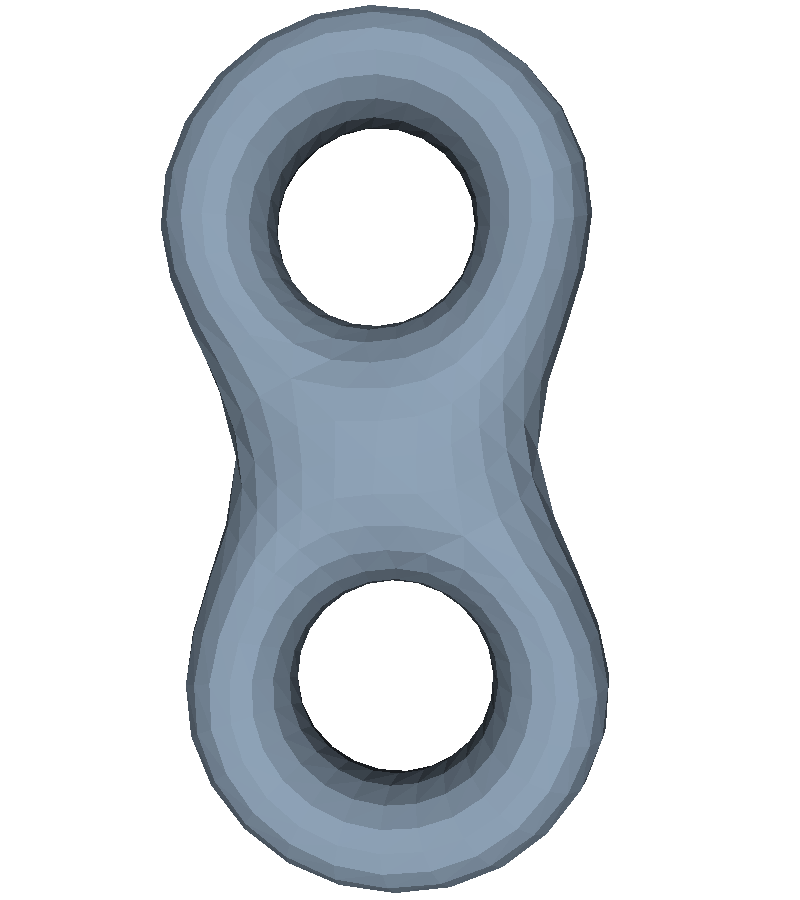
\includegraphics[width=\linewidth]{FIG1}
        \caption{} \label{fig:eight}
    \end{subfigure}%
    ~
    \begin{subfigure}[b]{0.35\linewidth}
        \includegraphics[width=\linewidth]{FIG2}
        \caption{} \label{fig:eight:coord}
    \end{subfigure}
    ~
    \begin{subfigure}[b]{0.35\linewidth}
        \includegraphics[width=\linewidth]{FIG3}
        \caption{} \label{fig:eight:spectral:coeff}
    \end{subfigure}%
    \\
    \begin{subfigure}[b]{0.4\linewidth}
        \includegraphics[width=\linewidth]{FIG4}
        \caption{} \label{fig:eight:spectral:energy}
    \end{subfigure}
    ~
    \begin{subfigure}[b]{0.4\linewidth}
        \includegraphics[width=\linewidth]{FIG5}
        \caption{} \label{fig:eight:spectral:approx:error}
    \end{subfigure}
    \caption[Approximation of the double-torus model with Laplacian eigenbasis.]
      {Approximation of the double-torus model with the Laplacian
      eigenbasis. (a) Original shape; (b) Vertex coordinate functions;
      (c) Spectral coefficients of the coordinate functions w.r.t. the
      Laplacian eigenbasis; (d) Ratios of spectral energy contained in
      the first $k$ coefficients; (e) Approximation error of the mesh
      geometry using the first $k$ coefficients.}
\label{fig:spectral}
\end{figure}

As an example, Fig.~\ref{fig:spectral} shows the power of Laplacian
eigenbasis for shape approximation. Fig.~\ref{fig:spectral}(b)-(c)
visualize the mesh coordinate functions of the example mesh and their
spectral transform coefficients, respectively. We can easily see that
the coordinate functions have very dense support in the natural graph
basis, but can be sparsely represented in the spectral/Fourier domain
in the sense that the majority of spectral coefficients are almost 0.
Moreover, the few significant coefficients are mostly concentrated in
the low-frequency end, especially for a smooth shape model.

Fig.~\ref{fig:spectral}(d) shows the spectral energies contained in
the first $k$ coefficients (linear approximation) and the first $k$
most significant coefficients (nonlinear approximation). We see that
the vast majority of spectral energy are captured by the first few
significant coefficients.

Fig.~\ref{fig:spectral}(e) shows how the mesh reconstruction error
changes with the number of coefficients being used. In this example,
we see that the approximation error becomes negligible using only
about 20 non-zero coefficients.

\subsection{Surface Inpainting}

In the previous section, we have shown that the geometry of a 3D shape
generally has a sparse representation w.r.t. its Laplacian
eigenbasis. Hence, we can set the Laplacian eigenvector as the
reconstruction dictionary and use the sparsity of coefficients as a
prior to estimate the representation of missing shape geometry.

Following the formulation in Sec.~\ref{sec:inpaint:model}, surface inpainting
can be rewritten as the following sparse approximation problem
\begin{equation}
\label{eq:sa}
\hat{\mathbf{\alpha}} = \arg\min_{\mathbf{\alpha}} \|\mathbf{\alpha}\|_0 \quad \text{s.t.} \quad \|P\Phi\mathbf{\alpha} - \mathbf{x}'\|_2^2 < \epsilon,
\end{equation}
\begin{equation}
\hat{\mathbf{x}} = \Phi \mathbf{\alpha}.
\end{equation}
Here the pseudo-norm $\|\mathbf{\alpha}\|_0 = \#\{ i : \alpha_i \neq
0\}$ denotes the support of $\mathbf{\alpha}$, which counts the number
of non-zero components of $\mathbf{\alpha}$, $\Phi$ denotes the
dictionary matrix comprising the Laplacian eigenfunctions, and
$\hat{\mathbf{x}}$ and $\mathbf{x}'$ represent the estimated and
observable coordinate functions, respectively.

We should note that, since the Laplacian eigenbasis constitute a
complete dictionary, Eq.~\ref{eq:sa} is solvable even if we set
$\epsilon=0$, in which case the reconstructed shape will exactly
match the known geometry. However, strictly sparse signals are rare in
real life. It is much more likely that the unknown shape geometry is
\emph{compressible} or \emph{weakly sparse} w.r.t. the dictionary of
Laplacian eigenvectors, i.e., the nonlinear approximation
errors observe a power law decay as the number of participating basis vectors
increases~\cite{Starck2010}. In practice, we set $\epsilon > 0$ to
trade off exact reproduction for a sparser $\alpha$, i.e., allowing the
reconstructed signal to have small discrepancies with the observation.

Solving $l_0$ optimization is an NP-hard problem in nature.
Fortunately, under certain conditions, greedy algorithms such as
orthogonal matching pursuit (OMP) and its variants can generate the
exact sparse solution or a good enough
approximation~\cite{Needell2010,Tropp2007}.

Another approach to find an approximated solution to Eq.~\ref{eq:sa}
is to relax the highly discontinuous $l_0$ norm with $l_1$ norm, i.e.
\begin{equation}
\label{eq:bpdn}
\hat{\mathbf{\alpha}} = \arg\min_{\mathbf{\alpha}} \|\mathbf{\alpha}\|_1 \quad \text{s.t.} \quad \|P\Phi\mathbf{\alpha} - \mathbf{x}'\|_2^2 < \epsilon,
\end{equation}
or equivalently,
\begin{equation}
\label{eq:bpdn2}
\hat{\mathbf{\alpha}} = \arg\min_{\mathbf{\alpha}} \|P\Phi\mathbf{\alpha} - \mathbf{x}'\|_2^2 + \lambda\|\mathbf{\alpha}\|_1.
\end{equation}

The estimation problem then becomes convex and solvable. There are
several readily available algorithms for solving $l_1$ optimization,
e.g., interior point method~\cite{Kim2007}, iteratively reweighted
least squares (IRLS)~\cite{Holland1977}, least angle regression
(LARS)~\cite{Sorkine2004}, and iterative
shrinkage-thresholding~\cite{Daubechies2004}.

For the task of surface inpainting, we find that $l_1$ optimization algorithms tend to be
more robust and generally produce better inpainting results than greedy algorithms. In this work,
we use the l1\_ls solver introduced in \cite{Kim2007} which implements a fast interior-point method
for solving $l_1$-regularized least-square problems like Eq.~\ref{eq:bpdn2}.

As an example, Fig.~\ref{fig:cube:random:inpaint} demonstrates the
potentials of our sparsity-based inpainting method. We randomly label
40\% of vertices of the original cube model as missing vertices, and
use the coordinates of the remaining vertices to estimate the spectral
coefficient representation of the original shape by solving
Eq.~\ref{eq:bpdn}. Fig.~\ref{fig:cube:random:inpaint}(b) shows the
shape reconstructed from the estimated spectral coefficients.
Fig.~\ref{fig:cube:random:inpaint}(c)-(d) shows the spectral
coefficients computed from the original x-coordinate function and the
coefficients estimated by our sparsity-based method, respectively. In
this example, our method recovers the sparse coefficient
representation in a very precise way.


\subsection{Filling Surface Holes}
\label{sec:inpaint:holefilling}

One of the most important technical elements of our surface inpainting
method is the dictionary of global shape basis, which are determined by
the global mesh connectivity. For some applications such as repairing
damaged surface regions, the mesh connectivity of the region to be
repaired is already known in advance before reconstruction and we may
not need to modify it. For hole filling applications, however, the
inpainting regions are completely blank without any inside
information. It is imperative to establish interior mesh connectivity,
by way of vertex insertion and patch triangulation, before our surface
inpainting method can be applied.

Obviously, how a patch (to be used to cover the hole region) is
triangulated directly influences the final inpainting result in our
framework. In general, a good patch triangulation should ensure the
vertex density of the inserted mesh to be consistent with the
remaining mesh. In this work, we adopt the algorithms proposed by
Liepa in \cite{Liepa2003} for hole triangulation and refinement.
Algorithm~\ref{algo:holefilling} summarizes the pipeline of our
sparsity-based hole filling method.

\begin{algorithm}
\caption{Sparsity-Based Hole Filling}
\label{algo:holefilling}
\begin{algorithmic}[1]
  \REQUIRE Input mesh $M$
\STATE Identify surface holes,
\STATE Triangulate and refine holes using the algorithms described in
  \cite{Liepa2003},
\STATE Compute the mesh Laplace matrix $L$ and the Laplacian eigenbasis dictionary $\Phi$,
\FOR{coordinate $\mathbf{x}$, $\mathbf{y}$, and $\mathbf{z}$}
\STATE Compute the spectral representation $\mathbf{\alpha}$ of the global coordinates by solving Eq.~\ref{eq:bpdn},
\STATE Reconstruct the coordinates of the inserted mesh with $\Phi\mathbf{\alpha}$,
\ENDFOR
\end{algorithmic}
\end{algorithm}

\subsection{Remarks on Dictionary}
\label{sec:inpaint:remark}

Although the dictionary of Laplacian eigenvectors in general has strong
compressive power for encoding shape geometry, it also has some limitations.
Similar to Fourier basis, the Laplacian eigenvectors are most suitable for
representing smooth signals or globally repetitive features, but are generally
not optimized for encoding shapes with many local sharp features. In the image
domain, other than 2D Fourier basis, people have developed various types of
harmonic basis (e.g., wavelet, curvelet, ridgelet, etc) for efficient encoding
of images of different properties. For example, the ridgelets are especially
efficient in representing piecewise smooth images with global straight
edges~\cite{Fadili2012}. In the mesh domain, however, we do not have such
diverse harmonic basis to choose from, which for now limits the power of
sparsity-based methods.

Another issue is related to the ratio of Laplacian eigen-decomposition.
Computing the full set of Laplacian eigenvectors of a large mesh is
extremely time consuming, generally infeasible for meshes with more than a few
thousand vertices on a regular PC. Fortunately, for our surface inpainting
applications, it is actually not necessary or even desirable to compute the
full set of eigenvectors. On the one hand, for smooth shapes, the spectral
energy is overwhelmingly concentrated on the low-frequency end, and a
dictionary composed of only low-frequency eigenvectors can well approximate the
shape geometry with very little error. On the other hand, the high-frequency
Laplacian eigenvectors are less stable than the low-frequency ones, and
including them in the dictionary may cause overfitting and result in worse
inpainting results, since the high-frequency eigenvectors are more correlated
with local geometric details than with the overall structure of the shape. In
our experiments, we find that the best inpainting results are usually achieved
with a dictionary of 20\% to 50\% total eigenvectors.

\begin{figure}
    \centering
    \begin{subfigure}[b]{0.36\linewidth}
        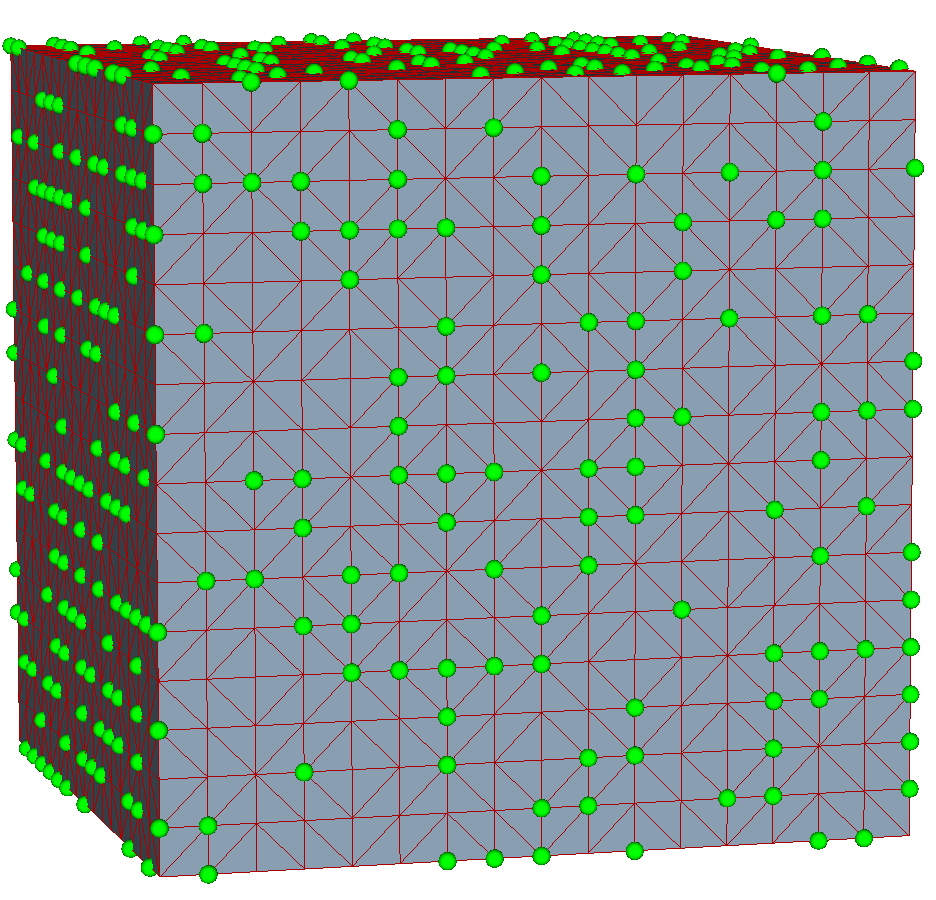
\includegraphics[width=\linewidth]{FIG6}
        \caption{}
    \end{subfigure}%
    ~
    \begin{subfigure}[b]{0.36\linewidth}
        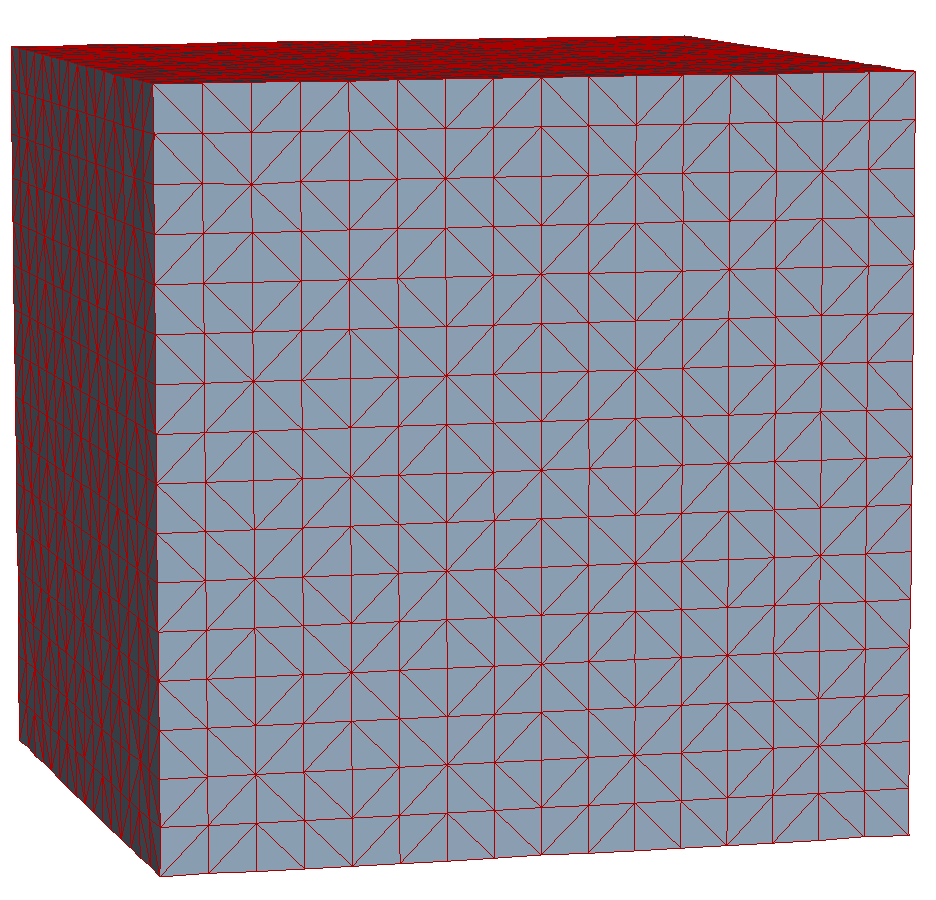
\includegraphics[width=\linewidth]{FIG7}
        \caption{}
    \end{subfigure}%
    \\
    \begin{subfigure}[b]{0.4\linewidth}
        \includegraphics[width=\linewidth]{FIG8}
        \caption{}
    \end{subfigure}%
    ~
    \begin{subfigure}[b]{0.4\linewidth}
        \includegraphics[width=\linewidth]{FIG9}
        \caption{}
    \end{subfigure}%
    \caption[Estimating Laplacian eigenbasis coefficients with partial cube model.]
      {Estimating the Laplacian eigenbasis coefficients of the
      cube model with 40\% random missing vertices. (a) Original shape model;
      green dots denote vertices that are labelled as missing. (b) The
      reconstructed shape using our inpainting method. (c) The
      coefficient representation of the original shape's
      x-coordinates. (d) Estimated coefficient representation of the
      x-coordinates inferred from the information of available
      vertices. }
\label{fig:cube:random:inpaint}
\end{figure}

\begin{figure}
  \centering
    \begin{subfigure}[b]{0.23\linewidth}
        \includegraphics[width=\linewidth]{FIG10}
        \caption{20\% vertices missing.}
    \end{subfigure}
    ~
    \begin{subfigure}[b]{0.23\linewidth}
        \includegraphics[width=\linewidth]{FIG11}
        \caption{Shape recovered from (a).}
    \end{subfigure}
    ~
    \begin{subfigure}[b]{0.23\linewidth}
        \includegraphics[width=\linewidth]{FIG12}
        \caption{50\% vertices missing.}
    \end{subfigure}
    ~
    \begin{subfigure}[b]{0.23\linewidth}
        \includegraphics[width=\linewidth]{FIG13}
        \caption{Shape recovered from (c).}
    \end{subfigure}
\caption[Recovery of the bunny model with random missing vertices.]
{Recovery of the bunny model with 20\% and 50\% random missing vertices.}
\label{fig:bunny:recovery}
\end{figure}

\begin{figure}
  \centering
    \begin{subfigure}[b]{0.23\linewidth}
        \includegraphics[width=\linewidth]{FIG14}
        \caption{20\% vertices missing.}
    \end{subfigure}
    ~
    \begin{subfigure}[b]{0.23\linewidth}
        \includegraphics[width=\linewidth]{FIG15}
        \caption{Shape recovered from (a).}
    \end{subfigure}
    ~
    \begin{subfigure}[b]{0.23\linewidth}
        \includegraphics[width=\linewidth]{FIG16}
        \caption{50\% vertices missing.}
    \end{subfigure}
    ~
    \begin{subfigure}[b]{0.23\linewidth}
        \includegraphics[width=\linewidth]{FIG17}
        \caption{Shape recovered from (c).}
    \end{subfigure}
\caption[Recovery of the horse model with random missing vertices.]
{Recovery of the horse model with 20\% and 50\% random missing vertices.}
\label{fig:horse:recovery}
\end{figure}

\begin{figure}
  \centering
    \begin{subfigure}[b]{0.23\linewidth}
        \includegraphics[width=\linewidth]{FIG18}
        \caption{20\% vertices missing.}
    \end{subfigure}
    ~
    \begin{subfigure}[b]{0.23\linewidth}
        \includegraphics[width=\linewidth]{FIG19}
        \caption{Shape recovered from (a).}
    \end{subfigure}
    ~
    \begin{subfigure}[b]{0.23\linewidth}
        \includegraphics[width=\linewidth]{FIG20}
        \caption{50\% vertices missing.}
    \end{subfigure}
    ~
    \begin{subfigure}[b]{0.23\linewidth}
        \includegraphics[width=\linewidth]{FIG21}
        \caption{Shape recovered from (c).}
    \end{subfigure}
\caption[Recovery of the fandisk model with random missing vertices.]
{Recovery of the fandisk model with 20\% and 50\% random missing vertices.}
\label{fig:fandisk:recovery}
\end{figure}

\begin{figure}
  \centering
    \begin{subfigure}[b]{0.23\linewidth}
        \includegraphics[width=\linewidth]{FIG22}
        \caption{20\% vertices missing.}
    \end{subfigure}
    ~
    \begin{subfigure}[b]{0.23\linewidth}
        \includegraphics[width=\linewidth]{FIG23}
        \caption{Shape recovered from (a).}
    \end{subfigure}
    ~
    \begin{subfigure}[b]{0.23\linewidth}
        \includegraphics[width=\linewidth]{FIG24}
        \caption{50\% vertices missing.}
    \end{subfigure}
    ~
    \begin{subfigure}[b]{0.23\linewidth}
        \includegraphics[width=\linewidth]{FIG25}
        \caption{Shape recovered from (c).}
    \end{subfigure}
\caption[Recovery of the centaur model with random missing vertices.]
{Recovery of the centaur model with 20\% and 50\% random missing vertices.}
\label{fig:centaur:recovery}
\end{figure}

\begin{figure}
    \centering
    \begin{subfigure}[b]{0.23\linewidth}
        \includegraphics[width=\linewidth]{FIG26}
        \caption{}
    \end{subfigure}%
    ~
    \begin{subfigure}[b]{0.23\linewidth}
        \includegraphics[width=\linewidth]{FIG27}
        \caption{}
    \end{subfigure}
    ~
    \begin{subfigure}[b]{0.23\linewidth}
        \includegraphics[width=\linewidth]{FIG28}
        \caption{}
    \end{subfigure}
    ~
    \begin{subfigure}[b]{0.23\linewidth}
        \includegraphics[width=\linewidth]{FIG29}
        \caption{}
    \end{subfigure}
\caption[Geometry repair of the damaged cube model.]
        {Geometry repair of the cube model by replacing the selected damaged regions (marked in yellow) with an inpainting patch.
         (a) The damaged model; (b) Repaired with Laplacian regularized least square smoothing~\cite{Nealen2006};
         (c) Repaired with thin-plate energy minimization~\cite{Bac2008};
         (d) Repaired with our inpainting method. In (b)-(d), the per-vertex error (compared with the ground truth) is color-coded.}
\label{fig:repair:cube}
\end{figure}

\begin{figure}
    \centering
    \begin{subfigure}[b]{0.23\linewidth}
        \includegraphics[width=\linewidth]{FIG30}
        \caption{}
    \end{subfigure}%
    ~
    \begin{subfigure}[b]{0.23\linewidth}
        \includegraphics[width=\linewidth]{FIG31}
        \caption{}
    \end{subfigure}
    ~
    \begin{subfigure}[b]{0.23\linewidth}
        \includegraphics[width=\linewidth]{FIG32}
        \caption{}
    \end{subfigure}
    ~
    \begin{subfigure}[b]{0.23\linewidth}
        \includegraphics[width=\linewidth]{FIG33}
        \caption{}
    \end{subfigure}
    \caption[Geometry repair of the damaged epcot model.]
    {Geometry repair of the damaged epcot model. (a) The original epcot model;
    (b) The damaged model (damaged region is marked in yellow); (c) Repaired with thin-plate
    energy minimization~\cite{Bac2008}; (d) Repaired with our inpainting method. In (c) and (d),
    the per-vertex error (compared with the ground truth) is color-coded. }
\label{fig:repair:epcot}
\end{figure}

\begin{figure}
    \centering
    \begin{subfigure}[b]{0.35\linewidth}
        \includegraphics[width=\linewidth]{FIG34}
        \caption{}
    \end{subfigure}%
    ~
    \begin{subfigure}[b]{0.35\linewidth}
        \includegraphics[width=\linewidth]{FIG35}
        \caption{}
    \end{subfigure}
    \\
    \begin{subfigure}[b]{0.35\linewidth}
        \includegraphics[width=\linewidth]{FIG36}
        \caption{}
    \end{subfigure}
    ~
    \begin{subfigure}[b]{0.35\linewidth}
        \includegraphics[width=\linewidth]{FIG37}
        \caption{}
    \end{subfigure}
    \caption[Geometry repair of the damaged wolf model.]
    {Geometry repair of the damaged wolf model.
         (a) The original wolf model; (b) Damaged model with significant noise in the region marked in yellow;
         (c) Repaired with Laplacian regularized least square smoothing~\cite{Nealen2006};
         (d) Repaired with our inpainting method. In (c) and (d), the per-vertex inpainting error (compared with the ground truth)
          is color-coded. }
\label{fig:repair:wolf}
\end{figure}

\begin{figure}
    \centering
    \begin{subfigure}[b]{0.45\linewidth}
        \includegraphics[width=\linewidth]{horse_error_vs_ratio}
        \caption{Horse model}
    \end{subfigure}%
    ~
    \begin{subfigure}[b]{0.45\linewidth}
        \includegraphics[width=\linewidth]{fandisk_error_vs_ratio}
        \caption{Fandisk model}
    \end{subfigure}
    \caption[Inpainting errors given different ratios of randomly missing vertices.]
    {Inpainting errors given different ratios of randomly missing vertices using our method. 
    The horse model uses 2,000 eigenvectors and the fandisk model uses 3,000 eigenvectors to
    construct dictionaries, respectively.}
\label{fig:error_vs_ratio}
\end{figure}

\section{Experiments}
In this section, we first evaluate the performance of our sparsity-based
inpainting algorithms on recovering missing geometry from partial observations.
Then we demonstrate how our method can be applied to repairing damaged geometry
and filling surface holes.

\subsection{Geometry Recovery}
To evaluate the performance of geometry recovery, for each testing model, we
randomly label 20\%-50\% vertices as missing and use our sparsity-based
inpainting method to estimate the original geometry based on the coordinates of
the still available vertices. The estimated coordinates are then compared with
the original coordinates.

All the testing models have been translated and scaled to be contained inside
the unit cube. The recovery error is measured as the
root-mean-square error (RMSE) of the coordinates of the missing vertices.

\begin{table}
\centering
  \begin{tabular}{|c|c|c|c|c|c|c|}
  \hline
  Mesh                     & \#vertices                 & \#eigenvectors          & \pbox{20cm}{Decomposition\\ time (s)}        & \pbox{15cm}{Missing\\ ratio} & Error  & $l_1$ time (s) \\
  \hline
  \multirow{2}{3em}{bunny} & \multirow{2}{4em}{2.5k}    & \multirow{2}{5em}{1000} & \multirow{2}{5em}{19.6}   & 0.2          & 1.9e-2 & 2.8       \\
                           &                            &                         &                           & 0.5           & 2.2e-2 & 2.1       \\

  \hline
  \multirow{2}{3em}{horse} & \multirow{2}{4em}{8.4k}    & \multirow{2}{5em}{4000} & \multirow{2}{5em}{1015.4} & 0.2          & 8.6e-3 & 19.7      \\
                           &                            &                         &                           & 0.5           & 1.0e-2 & 59.0      \\
  \hline
  \multirow{2}{3em}{fandisk} & \multirow{2}{4em}{6.5k} & \multirow{2}{5em}{3000} & \multirow{2}{5em}{445.2}   & 0.2          & 8.8e-3 & 17.4      \\
                             &                          &                         &                           & 0.5           & 1.2e-2 & 33.9      \\
  \hline
  \multirow{2}{3em}{centaur} & \multirow{2}{4em}{15.8k} & \multirow{2}{5em}{2000} & \multirow{2}{5em}{397.7}  & 0.2          & 7.1e-3 & 12.2      \\
                             &                          &                         &                           & 0.5           & 8.0e-3 & 15.0      \\
  \hline
  \end{tabular}
\caption[Geometry recovery errors and time performance.]
{Geometry recovery errors and time performance. For each model, we test the recovery performance with
20\% and 50\% randomly selected vertices labelled as missing. Each experiment has been repeated three times
and averaged on a system with quad-core 2.4GHz CPU and 16GB RAM. }
\label{tab:recovery}
\end{table}

Fig.~\ref{fig:bunny:recovery}, Fig.~\ref{fig:horse:recovery}, Fig.~\ref{fig:fandisk:recovery}, and Fig.~\ref{fig:centaur:recovery}
show some examples of geometry recovery with 20\% and 50\%  missing vertices. Fig.~\ref{fig:error_vs_ratio} shows
two examples of how the inpainting error (MSRE) changes with the ratio of vertices randomly labeled as missing. 

Table~\ref{tab:recovery} documents
the recovery errors and time performance of our tests. From the experimental results, we have the following
observations:

\begin{itemize}
  \item When the missing vertices are randomly dispersed on the shape, our
        sparsity-based method can reliably recover the missing coordinates
        with great precision, even when the ratios of missing vertices are
        as high as 50\%.
  \item The $l_1$ estimation generally becomes more time consuming when the
        ratio of missing vertices increases.
  \item As noted in Sec.~\ref{sec:inpaint:remark}, using the truncated Laplacian
        eigenbasis dictionary is acceptable for restoring smooth shapes.
        However, for shapes with many edges and corners, such as the fandisk
        model (see Fig.~\ref{fig:fandisk:recovery}), our inpainting method
        cannot well preserve local discontinuities, since the high-frequency
        basis are simply not present in the truncated dictionary.
\end{itemize}

\subsection{Geometry Repair}
Our sparsity-based inpainting method is very suitable for repairing partially
damaged geometry. After manually selecting the damaged regions, we can apply
our inpainting method to estimate the original whole shape with the same
connectivity based on the remaining parts of the shape. The corrupted regions
can then be substituted by the inpainting patch.

Fig.~\ref{fig:repair:cube}, \ref{fig:repair:epcot}, and \ref{fig:repair:wolf}
demonstrate repairing damaged local geometry using our sparsity-regularized
inpainting method. The results are compared with two geometry-regularized mesh
optimization methods: Laplacian regularized least square
smoothing~\cite{Nealen2006} and thin-plate energy minimization~\cite{Bac2008}.
We can see that, although geometry-regularized methods can generate patches
that are smooth and blend well with the surroundings, they fail to recognize
the intrinsic structures of the original shapes; consequently, important
geometric features are simply smoothed out. In contrast, our
sparsity-regularized inpainting method takes into account the global shape
structures, and almost perfectly recovers the edges and corners in the cube
model (Fig.~\ref{fig:repair:cube}) and the geometric textures of the epcot
model (Fig.~\ref{fig:repair:epcot}) from partial observations.


\subsection{Hole Filling}

As introduced in Sec.~\ref{sec:inpaint:holefilling}, for general hole filling
tasks, the mesh connectivity information inside holes are probably unknown. We
must first triangulate holes in a proper way and then apply our geometry
inpainting method to optimize the newly inserted mesh. How the hole is
triangulated directly impacts the global Laplacian eigenbasis which subsequently
determine the estimated recovery.

As an example, Fig.~\ref{fig:holefilling1} compares the results of filling the
holes of a double torus model with and without original connectivity
information, using our sparsity-regularized method and the geometry-regularized
method proposed in \cite{Bac2008}. We can see that estimating with a different
connectivity significantly alters the final hole fairing results. In this
example, our method generate shapes that are more approximate to the original
shape both with the original connectivity and with the new connectivity.

\begin{figure}
\centering
    \begin{subfigure}[b]{0.3\linewidth}
    \includegraphics[width=\linewidth]{FIG38}
    \caption{}
    \end{subfigure}
    ~
    \begin{subfigure}[b]{0.3\linewidth}
    \includegraphics[width=\linewidth]{FIG39}
    \caption{}
    \end{subfigure}
    ~
    \begin{subfigure}[b]{0.3\linewidth}
    \includegraphics[width=\linewidth]{FIG40}
    \caption{Error: 0.010}
    \end{subfigure}
    \\
    \begin{subfigure}[b]{0.3\linewidth}
    \includegraphics[width=\linewidth]{FIG41}
    \caption{Error: $4.1\times 10^{-4}$}
    \end{subfigure}
    ~
    \begin{subfigure}[b]{0.3\linewidth}
    \includegraphics[width=\linewidth]{FIG42}
    \caption{Error: 0.030}
    \end{subfigure}
    ~
    \begin{subfigure}[b]{0.3\linewidth}
    \includegraphics[width=\linewidth]{FIG43}
    \caption{Error: 0.021}
    \end{subfigure}
\caption[Comparison of hole filling results using sparsity-regularized method and geometry-regularized method.]
        {Compare hole filling results using our sparsity-regularized method and the geometry-regularized method introduced in ~\cite{Bac2008}.
        The error is measured as the root-mean-squared deviation from the estimated vertices to the original shape.
        (a) The original double torus model.
        (b) The model with a hole.
        (c) Inpainted using the method in \cite{Bac2008} with the original mesh connectivity.
        (d) Inpainted using our method with the original mesh connectivity.
        (e) Inpainted using the method in \cite{Bac2008} with the mesh connectivity generated from hole triangulation and refinement.
        (f) Inpainted using our method with the same mesh connectivity as (e).}

\label{fig:holefilling1}
\end{figure}

In general cases, we cannot expect the hole filling result using our
sparsity-regularized inpainting method to precisely match the original shape
when the number of vertices and connectivity of the patching mesh, generated
from hole triangulation and refinement, are different from the original mesh.
Nonetheless, the resulting patching meshes tend to be coherent with the whole
remaining shape, thanks to the global shape awareness of our method.
Fig.~\ref{fig:holefilling2} shows two examples of filling holes utilizing our
inpainting method. The results are comparable to the geometry-regularized
surface restoration method in \cite{Bac2008}.

\begin{figure}
\centering
    \begin{subfigure}[b]{0.33\linewidth}
        \includegraphics[width=\linewidth]{FIG44}
        \caption{}
    \end{subfigure}%
    ~
    \begin{subfigure}[b]{0.33\linewidth}
        \includegraphics[width=\linewidth]{FIG45}
        \caption{}
    \end{subfigure}%
    ~
    \begin{subfigure}[b]{0.33\linewidth}
        \includegraphics[width=\linewidth]{FIG46}
        \caption{}
    \end{subfigure}
    \\
    \begin{subfigure}[b]{0.33\linewidth}
        \includegraphics[width=\linewidth]{FIG47}
        \caption{}
    \end{subfigure}%
    ~
    \begin{subfigure}[b]{0.33\linewidth}
        \includegraphics[width=\linewidth]{FIG48}
        \caption{}
    \end{subfigure}%
    ~
    \begin{subfigure}[b]{0.33\linewidth}
        \includegraphics[width=\linewidth]{FIG49}
        \caption{}
    \end{subfigure}
\caption[Hole inpainting on the bunny and hand models.]
        {Inpainting existing holes on the bunny and hand models. (a)(d) Original models with holes;
        (b)(e) Hole-filling result using our method;
        (c)(f) Hole-filling result using the method of \cite{Bac2008}.}
\label{fig:holefilling2}
\end{figure}

\section{Chapter Summary}
In this chapter, we have proposed a novel surface inpainting algorithm based on
sparse signal recovery. Instead of directly estimating the local missing
geometry, our new inpainting framework is designed to discover the coefficient
representation of the entire original shape in a transform domain. When the
shape geometry is sufficiently sparse with respect to the dictionary of
transform basis, chances are we can accurately recover this sparse
representation by imposing sparsity constraints on the coefficients given
partial observations. In our method, we adopt the mesh Laplacian eigenbasis as
dictionary, and formulate surface inpainting as a sparse signal recovery
problem. Leveraging standard $l_1$ optimization techniques, we can obtain an
estimated shape which agrees with the observable parts and are globally
coherent. For shapes that are highly compressible w.r.t. the Laplacian
eigenbasis, we have experimentally demonstrated the great potential of our
method for geometry restoration, geometry repair, and hole filling.

For the future work, we plan to extend our sparsity-based inpainting framework
by integrating geometric constraints such as curvatures and normals, which
should improve the geometric consistency of the inpainting result. We are also
interested in designing new types of shape basis and exploring more
sophisticated strategies for constructing dictionaries, e.g., dictionaries that
are adaptive to the input shape. 
\graphicspath{{fig-feature/}}
\chapter{Generalized Feature Description and Detection}
\label{chap:feature}

\section{Introduction}
Studies in feature abstraction and analysis have been gaining momentum because
features are essential for numerous downstream graphics tasks and applications
such as shape recognition, segmentation, analysis, understanding, etc
~\cite{Bronstein2011,Kin-ChungAu:2012,Song:2014:MSV}. Influenced
by the trending concept of high-level representations in computer
vision, which are based on object-wise components, more
attention has now been directed towards region-wise feature analysis in
geometry modeling. In this work, we advocate a new region-based and
user-specified type of feature as well as a novel
wavelet-inspired multi-scale and multi-level descriptor, and they
jointly enable our feature detection framework that can further
facilitate various applications.

Conventional feature descriptors are usually constructed by considering
the discontinuities of certain differential attributes of different
orders (e.g., the second-order attribute like surface curvature) that
naturally afford their discriminative power in characterizing point
features, line/curve features, small patch-based features with regular
boundaries, etc. Such descriptions have been employed in point/patch-based
recognition, point-wise correspondence, and curvature-based saliency
detection with great success. However, for more complicated applications
such as modeling by example~\cite{Funkhouser:2004}, model
composition~\cite{Kreavoy:2007}, and key component
analysis~\cite{Sipiran:2012}, the aforementioned conventional features
are usually too localized to capture the multi-scale neighboring
information, and it is desirable to have a flexible, region-induced feature
description. Furthermore, in many real-world settings, shape data may be
degraded due to acquisition imperfections and noises, necessitating the
use of region descriptors which tend to be much more robust.

Existing works related to region-wise analysis include partial matching,
shape correspondence, saliency extraction, etc. Boundaries of the regions
in question are usually confined to regular but non-adaptive
shapes~\cite{Kazhdan:2003,Mortara:03,Gatzke:2005,Kokkinos:2012}, thus
neighboring and in-between geometry information may not be fully captured.
As for region description, trending measures include the distributions of
various types of point
descriptors~\cite{Osada:2002,Ben-Chen:2008,Liu:2006} and the global
analysis of the regions based on spectral
decomposition~\cite{Hu2009,Lavoue:2012}. Some regional measures are
not discriminative enough to solely characterize the regions in question,
for which post-processing like geometric
hashing~\cite{Yehezkel:1988} or random sample
consensus~\cite{Fischler:1981} is required. Nevertheless, these settings
are not hierarchical enough to characterize the focal regions. On the
other hand, multi-scale shape analysis
methods~\cite{Rustamov2011,Sun:2009:CGF}, in spite of their great
descriptive power, have not yet been employed to construct regional
descriptions. These insights inspire us to propose a more comprehensive
and stable type of shape description that can encode the region of
interest with high discriminative power and efficiency.


\begin{figure}[!to]
\begin{center}
\includegraphics[width=1\linewidth]{Fig_1}
\end{center}
\caption[Pipeline of our generalized feature detection framework.]
{Pipeline of our feature detection and description framework.}
\label{pipeline}
\end{figure}

In this chapter, we propose a local-to-global shape feature via user
specification, introduce an informative region descriptor, and then
present a shape feature detection framework to facilitate a host of
graphics applications. The proposed shape feature extends the
definition of conventional features to a region-wise manner in a
user-specified way (as highlighted in Fig.~\ref{pipeline}). To encode
user-specified features, we proactively seek an informative regional
descriptor constructed in a multi-scale and multi-level way. Our
descriptor takes advantage of the bi-harmonic distance field and the
SGWs. The stability and robustness of bi-harmonic distance field
guarantee the technically-sound foundation for the whole descriptor.
SGWs naturally accommodate local and global geometry with a
multi-scale solution, and such solution is consistent across multiple
levels. We devise a new statistical method based on the decomposition
coefficients of the shape signal, enabling the joint analysis of the
underlying geometry together with different shape signals. In order
to comprehensively characterize the shape features, we also
incorporate the contour-centered geometric statistics into our
descriptor. All of these enable our feature detection framework as
shown in Fig.~\ref{pipeline}. We quantify each model's regions of
interest around central points (or point samples) according to the
user-specified feature scope on the query model. Then descriptors are
constructed on candidate regions across different models, which is
equivalent to transform each region into the high-dimensional feature
space. After the region-wise feature space is constructed, various
analytical tasks can be performed. The primary contributions of this
work can be summarized as follows:

\begin{itemize}
\item We propose to define a generalized shape feature type via user
    specification, which is geometry-aware and is the organic coupling
    of local and global description. Also, it is a fundamental tool
    that can help unite different types of graphics applications.

\item Our region-based descriptor is primarily built upon the SGWs
    that are both multi-scale and multi-level in nature, elegantly
    integrating both local (differential) and global (integral)
    information. We also introduce the contour-centered geometric
    statistics to enhance the descriptor's discriminative power.

\item We develop a feature detection framework, which can integrate
    different types of state-of-the-art region descriptors and further
    facilitate widespread graphics applications including partial
    matching, coarse-to-fine recognition, model recognition, etc.

\end{itemize}

\section{Related Work}
\label{sec:RW}

This section will briefly review prior research related to region
analysis and the latest progresses on SGWs.

\textbf{Region-wise Description and Detection.} We first review how
current methods define boundaries for given regions. Broadly speaking,
they characterize a local neighborhood around a central point in two
ways. The first is based on Euclidean distance, such as
spheres~\cite{Kazhdan:2003}, blowing bubbles~\cite{Mortara:03},
rings~\cite{Gatzke:2005}, shape context~\cite{Kokkinos:2012} or priori
decompositions~\cite{Gal2006,Itskovich2011}. The second is to use
geodesic distance like geodesic fans~\cite{Zelinka:2004} and spiral
pathway~\cite{Lavoue:2011}. The shapes of region boundaries defined by
the above methods are mostly restricted to regular formats, and such
nonadaptive neighborhoods cannot precisely reflect the local
geometrical or topological distortions. Region-wise descriptors can be
roughly divided into two categories: point-based and region-based
methods. Point-based methods provide the quantitative measure by
organizing single-valued point signatures into certain kinds of
distributions. Various kinds of point descriptors have been
incorporated in this manner, e.g., the shape index
(SI)~\cite{Toldo:2009}, shape diameter function
(SDF)~\cite{Shapira:2010}, heat kernel signature
(HKS)~\cite{Bronstein:2013}, Zernike
moments~\cite{Maximo:2011:RRI:2027471}, etc. Region-based methods
analyze the entire focal region through spectral
decomposition~\cite{Hu2009,JiangZZ:13}, which can robustly depict the
intrinsic geometry. However, due to the instability of local Laplacian
decomposition, these methods usually cannot well handle small and
complex regions.

\textbf{Region-based Partial Matching and Correspondence.} In
literature, region analysis has been discussed mainly in the research
of partial matching problems, and several categories of techniques
have been employed. Skeletal-graph-based approaches such
as~\cite{Biasotti:2006} couple geometry and structure in a single
skeletal descriptor based on the theory of Reeb graph. The main
drawback is that sub-parts cannot be recognized automatically.
Multi-criterion optimization
approaches~\cite{Bronstein:2008,Castellani:2008,Lavoue:2011} try to
match subparts by striking balance between significance and
similarity criteria. This type of methods require the knowledge of
correspondence between shapes, otherwise, it can only be solved by
alternating between correspondence and part area, which is
time-consuming. Bag-of-words (BoWs) technique has been
adopted~\cite{Zaharescu2009,Bronstein:2010:CVPR} to represent a shape or a
subpart as a collection of local feature signatures quantized in some
vocabularies of ``geometric words''. If the geometric vocabulary is
sufficient and the shapes have significant common parts, it is
possible to compare partially-similar shapes, otherwise, these
methods oftentimes fail to function properly. Furthermore, improper
additions of the spatial information and imprecise binning process
may lead to the averaging-off effects of geometric information. The
concept of non-point-wise correspondence was first proposed
in~\cite{Bronstein:2013} by using region-wise local descriptors and
optimizing over the integration domain upon which the integral
descriptors of the two parts match. This method can exactly match
fragments to entire shapes, however, since it utilizes the absolute
values in calculation like integration, it cannot deal with the
partially similar correspondence. Besides, many of the above
approaches rely heavily on exact or meaningful shape decomposition
process as in~\cite{Itskovich2011,Lavoue:2012}, which is
computationally expensive and significantly influences the final
correspondence results. Also, in order to achieve meaningful results,
many approaches utilize time-consuming post-processing like
in~\cite{Gal2006} and~\cite{Itskovich2011}. So it requires more
effective and generalized region detection techniques to help speed
up and improve the precision of the partial matching and
correspondence processes.

\begin{figure*}
\begin{center}
\includegraphics[width=0.68\textwidth]{Fig_2}
\end{center}
\caption[Illustration of the steps of our feature detection framework.]
  {The functional pipeline of our feature detection framework.
  (a)-(c) show the user's inputs in the specification process, red
  arrows in (a) and (b) denote the specified point of interest and
  contour scope, respectively. The bottom row shows the specified
  shape feature (e) and analogous feature regions (d) (we only
  display three cases here).}
\label{specification}
\end{figure*}

\section{Local-to-global Shape Feature Definition}
\label{sec:GF}

In this section, we introduce the definition process of the proposed
novel shape feature, which generalizes conventional features (e.g.,
point, line, or patch features) to a local-to-global level via user
specification. Our shape feature is extracted via the bi-harmonic
distance field~\cite{Lipman:2010}, which is robust, globally
``shape-aware'', parameter-free, and widely used in geometry
processing. Among these attractive properties, the consecutive
depicting power inspires us to incorporate it for integrating
multi-scale regional information that is required for subsequent
analysis. In addition, the cross-sections of contours in the
bi-harmonic distance field naturally form boundaries for
user-specified features, thus avoiding the shape decomposition
process.

Our shape feature is a user-specified partial region with two
parameters: the point of interest and the contour scope, both of
which can be determined using a simple user-interactive process. The
point of interest is the relative center of the feature, it can either
be picked directly on the mesh, as shown in
Fig.~\ref{specification}(a), or be automatically initialized as the
extreme point of a function defined on the surface. In order to specify
the contour scope of the point of interest, we should first introduce
the metric with which we set the scope, namely, the bi-harmonic
distance field.

Let us consider a 3D mesh represented as a graph $M = (V;E)$ with
vertices $V$ and edges $E$, where $V = \{v_1,v_2,...,v_n\}$ and $n$ is
the number of the vertices. A vector-valued function $f \colon
\textbf{V} \rightarrow \mathbb{R}^q $ defined on $V$ can be
represented as an $n \times q$ matrix, where the $i$-th row represents
the function value at $v_i$, we denote it as $f(i)$. According
to~\cite{Lipman:2010}, the bi-harmonic distance between vertex $v_i$
and $v_j$ can be expressed as
\begin{equation}
\label{eq:bd}
D_{bh}(i,j)^2=\sum_{k=1}^{m}\frac{(\chi_k(i)-\chi_k(j))^2}{\lambda_k^2},
\end{equation}
where $\{\lambda_k\}$ and $\{\chi_k(\cdot)\}$ are, respectively, the
first $m$ non-zero eigenvalues and the corresponding eigenfunctions of
the Laplacian-Beltrami operator with ``cotangent formula''
discretization~\cite{Meyer2003}.

For each vertex, Eq.~(\ref{eq:bd}) defines a diffusion field around
it. We compute the diffusion field of the specified interest point
(denoted as $v_s$) and then construct a set of contours
(Fig.~\ref{specification}(b)) across the entire model with contour
points located on the edges of the mesh model. These contours can very
well reflect the changes locally around the central point and
characterize the corresponding global structures, and these will be
discussed later. In order to make the setting of parameters more
stable, we normalize the original models using a unit box. Then the
total number of the contours distributed in the diffusion field can be
set empirically to the integer nearest to $max(D_{bh}(s,\cdot))/0.05$,
which is dense enough to depict the diffusion field. Then the user can
choose one of the contours to set the scope of the feature (as shown
in Fig.~\ref{specification}(b)) and denote it as $S_{s}$.
Fig.~\ref{specification}(c) illustrates the feature defined with the
red boundary.

Our shape features can be located anywhere and vary spatially in scale
depending on specific applications. They integrate the local and global
geometry, which affords their great potential in bridging differential
and integral geometry information.

\section{Multi-level And Multi-scale Shape Description}
\label{sec:Des}

Our novel descriptor primarily make use of the statistics
of SGWs coefficients. As a supplement, contour-based statistics are also
included the descriptor to achieve better discriminative power.

\subsection{SGW-based Description}

As mentioned in Chapter~\ref{chap:background}, spectral graph wavelet transform (SGWT)
defines a new type of wavelet analysis on graphs by performing scaling of mother wavelet
in the Fourier domain instead of the spatial domain. The SGWs are expressed as bivariate
kernel functions expanded on the manifold harmonic basis
\begin{equation}
\label{eq:SGW}
\Psi_{t}(i,j)=\sum_{k=0}^{n-1}g(t\lambda_k) \chi_k(i)\chi_k(j),
\end{equation}
where $g$ is the real-valued wavelet generating kernel and $t$ is the
scale parameter. The $i$th row of $\Psi_{t}(\cdot,\cdot)$
\begin{equation}
\label{eq:SGW_vert}
\psi_{t,i}(\cdot) = \Psi_{t}(i,\cdot)=\sum_{k=0}^{n-1}g(t\lambda_k) \chi_k(i)\chi_k(\cdot),
\end{equation}
is the spectral wavelet spatially-localized at $v_i$, and in the
frequency domain, localized at scale $t$. It should be noted that
we choose to use the geometric mesh Laplacian for more geometric-aware
description, instead of the combinatorial Laplacian originally used
in~\cite{Hammond2011}.

Multi-scale SGWs can well represent both the high frequency and low frequency
geometric information around the index point.  Suppose we
compute the spectral wavelets at $J$ different scales $\{t_1,t_2,...,t_J\}$,
and adopt the same formulation of generating kernel functions used
in~\cite{Hammond2011}, given by
\begin{equation}
g(x)=\left\{
\begin{array}{lcl}
x^2                &      & {if\  x<1}\\
-5 +11x-6x^2 +x^3  &      & {if\  1 \leq x \leq 2}\\
4x^{-2}            &      & {if\  x>2}\\
\end{array} \right.,
\end{equation}
and the $J$ scales are selected to be logarithmically equally spaced
between the minimum scale $t_J = 2/\lambda_{max}$ and the maximum
scale $t_1=40/\lambda_{max}$, where $\lambda_{max}$ is the upper bound
of the Laplacian eigenvalues. The settings of $t_1$ and $t_J$
guarantee that $g(t_1 x)$ has power-law decay for $x>\lambda_{min}$
and $g(t_J x)$ has monotonic polynomial behavior for $x<\lambda_{max}$.

Using the above formulations, we can easily obtain the wavelet
coefficients of a given function centered on a specific vertex $v_i$ as
\begin{equation}
\label{eq:WMD}
W_f(t,i) = \langle \psi_{t,i},f \rangle = \sum_{l=0}^{n-1}g(t\lambda_l)\hat{f}(l)\chi_l(i),
\end{equation}
where
\begin{equation}
  \hat{f}(l) = \langle \chi_l,f \rangle.
\end{equation}

Here, the signal function $f$ can be any kind of surface signal
depending on the downstream application. For example, mean curvature,
characterizing detailed local distortions, is a good choice for the
recognition of repetitive features within individual models and the
detection of similar features across models with different poses.
For coarse-to-fine recognition, the HKS is more favorable thanks to
its robustness to noise. The coefficients $W_f$
obtained from the spectral wavelet transform is the inner product of the signal
function and the corresponding wavelet at scale $t$ and location $i$.
It is an encoding of the signal at that particular scale, i.e.,
it describes the original signal in certain frequency with respect to
the local geometry and topology. Repeating this process for $J$
scales (as shown in Fig.~\ref{wmd}(a)-(d) with 4 scales), the collection of
coefficients obtained comprises our multi-level and multi-scale descriptor.

\begin{figure}[!to]
\begin{center}
\includegraphics[width=0.9\linewidth]{Fig_4}
\end{center}
\caption[Statistics on wavelet decomposition coefficients.]
  {Statistics on signal's wavelet decomposition coefficients
  ($W_f(\cdot,t)$). (a)-(d) list $t$ from small ($t_1$) to large
  ($t_4$) value, corresponding to the decomposed signals varying from
  high to low frequencies. (e) illustrates the composition of
  statistics based on $W_f$ within one feature region.}
\label{wmd}
\end{figure}

Instead of using $W_f$ directly as descriptors like in \cite{Li:2013}, 
we incorporate it into our descriptor by taking advantage of the
consecutive depicting power of the bi-harmonic distance field. In
order to comprehensively describe the geometric information contained
within the feature, we divide the feature region into thinner bands
with more contours as shown in Fig.~\ref{specification}(c)-(e). 
The number of dense contours may be set automatically as the integer nearest 
to $S_{s}/0.025$, and such dense contours can elaborately depict and 
organize the inner geometrical information within the feature
region. Fig.~\ref{wmd}(e) illustrates the setup of our SGW-based statistical
bands based on $W_f$, where different layers convey multi-level (from
high to low frequency) information and different bands (denoted in
yellow and green) in-between contours encode multi-scale information.
By stretching the ``matrix-like" statistic (as in Fig.~\ref{wmd}(e))
into a high dimensional vector, we obtain the descriptor of $v_s$,
denoted as $D_s$, given by
\begin{equation}
\label{eq:Des}
\hspace{-1.2mm}
D_s=[\underline{W_{t_1}^{b_1},...\ ,W_{t_1}^{b_L}},\\
\underline{W_{t_2}^{b_1},...\ ,W_{t_2}^{b_L}},\\
\underline{...}\ , \\
\underline{W_{t_J}^{b_1},...\ ,W_{t_J}^{b_L}}],
\end{equation}
where $W_{t_i}^{b_j}$ denotes the statistic of $W_f$ with scale $t_i$
on the $j$-th band, and $L$ is the number of contours. Here
$W_{t_i}^{b_j}$ can be expressed as the 1-norm of $W_f(t_i, \cdot)$
over the $j$-th band
\begin{equation}
\label{eq:WMD_sta}
W_{t_i}^{b_j} = \sum_{p \in b_j}| W_f(t_i,p)|,
\end{equation}
where $p$ is the vertex index, $p \in b_j$ denotes $p$ is a vertex
located on the $j$-th band.

In Fig.~\ref{wmd}, we observe that information contained in $W_f$ of
different time scales corresponds to the fine-to-coarse multi-level
information, and the statistics on the bands convey the near-to-far
multi-scale knowledge. These collectively make use of SGWs' power in
integrating geometric information. In addition, we notice that
descriptors based on $W_f$ are scale-invariant as long as SGWs are
normalized.

\subsection{Contour-based Multi-scale Statistics}

\begin{figure}[!to]
\begin{center}
\includegraphics[width=0.8\linewidth]{Fig_5}
\end{center}
\caption[Contour-based distance distribution.]
  {Contour-based distance distribution. The zoomed-in part
  shows the distances under current consideration when performing
  statistical calculation.}
\label{Descriptor}
\end{figure}

The contours of bi-harmonic distance field encode rich information of
local-to-global geometric variation. So we further introduce the
perimeters of contours and the distance distribution of contour points
to help characterize the focal region's shape in an orderly and
quantitative manner.

For a specified feature and its corresponding contours, we first
calculate contours' perimeters and concatenate them as
$\{p^{c_1},p^{c_2},...,p^{c_L} \}$, where $c_i$ denotes the index of
the $i$-th contour. Then, for each contour, we compute the Euclidean
distances between the contour points and their barycenter (as shown in
Fig.~\ref{Descriptor}), and further evaluate the probability
distribution of the distances. We denote the distance-related
statistics as $\{ds^{c_1},ds^{c_2},...,ds^{c_L} \}$. Here, $ds^{c_i}$
is a vector stacking up the probability distribution of the distances
concerning the $i$-th contour. We uniformly separate the distance
values into $M$ bins, ranging from zero to the maximum value after
removing the top and bottom 5\% to rule out possible outliers. Then
its stack pattern is
\begin{equation}
  ds^{c_i}=[\frac{num(b_1)}{num(c_i)},\frac{num(b_2)}{num(c_i)},...,\frac{num(b_M)}{num(c_i)}],
\end{equation}
where $num(b_j)$ is the number of points with distance values falling
in the $j$-th bin and $num(c_i)$ is the number of points on the $i$-th
contour. For multiple contours with the same value, they should be
considered as a whole when performing statistical calculation.

These two measurements help describe the shape of the bi-harmonic
distance field completely and identify the details of shape's
distortion. The purpose of introducing the distance distribution is
to distinguish between different contours with the same perimeters.

\subsection{Informative Region-based Descriptor}

So far, the separate parts of our descriptor have all been introduced.
Now, it sets the stage for us to integrate them together to form our
final informative hi-dimensional descriptor as
\begin{equation}
\label{eq:desFinal}
\begin{aligned}
  \hspace{-0.5mm}
  D_s =  [\omega_s*(W_{t_1}^{b_1},...\ ,W_{t_J}^{b_L}),\\
  \omega_p*(p^{c_1},...\ ,p^{c_L}),\\
  (ds^{c_1},...\ ,ds^{c_L})],
\end{aligned}
\end{equation}
where $\omega_s$ and $\omega_p$ are weights to adjust the
contributions of the three parts in the descriptor. The settings of
these weights will be detailed in Section~\ref{sec:Exp}.

Our descriptor integrates the attractive properties of both SGWs and
contour-based measurements. From the viewpoint of feature mapping,
SGWs establish a powerful foundation for hierarchical representation
of the geometrical and topological details. Our design of the
regional description encodes the shape feature in the aspects of both
``breadth'' and ``depth'', paving the way for our feature detection
framework.

\section{Feature Detection Framework}
\label{sec:Framework}

Using the same way to define feature regions around candidate points
and formulate the corresponding descriptions, descriptors concerning
candidate regions on the same model or different models in the
database can be easily computed for analytical purposes.

\subsection{Constructing Descriptors over Shapes}

To construct descriptors on candidate regions on one or more models,
the central points and contour scopes should also be determined first.
As for the central points, we implement the farthest-point-sampling
strategy~\cite{Moenning:2003} to uniformly extract points on the mesh
model (as shown in Fig.~\ref{Sampling}). This strategy ensures not
only the uniform distribution of the candidate points, but also the
inclusion of the end points, which are interesting alternatives for
user's selection. However, we want to mention that the sampling
process is optional, and users could either pick the desired sampling
methods or simply use all the vertices as candidates according to
specific applications.

Then the construction of descriptors across versatile shapes is based
on the knowledge of the shape feature defined. That is, candidate
regions are determined automatically according to the contour scope of
the shape feature specified. Suppose that $v_{s}$ and $v_{i}$ are
respectively the interest point and one of the candidate points. Then
the scope of $v_{i}$ is set as
$S_{s}*max(D_{bh}(i,\cdot))/max(D_{bh}(s,\cdot))$ and this can help
ensure the robustness of our method for deformable models.  With the
region scope determined, the construction of the corresponding
descriptor is conducted in the same way as the specified feature (in
Section~\ref{sec:Des}), which is detailed in
Algorithm~\ref{alg:Framwork}.

\begin{figure}[!to]
\begin{center}
\includegraphics[width=0.9\linewidth]{Fig_6}
\end{center}
\caption[Point sampling on the horse and Santa models.]
  {Sampling results on horse and Santa models using the
  farthest-point-sampling strategy. Only part of the sampling points
  are shown for visual clarity.}
\label{Sampling}
\end{figure}

With each candidate region equipped with a high-dimensional
descriptor, our key task is to analyze the similarity in the
descriptor space. We shall first introduce the proper measurements
for this new space. It has been found that both $L1$ and $L2$ norms
are discriminative enough to measure the distance between any two
descriptors, representing the corresponding regions. As alternatives,
the covariance distance and $\chi{2}$ distance are also tested to be
good choices for comparing the distributions' similarities.

\subsection{Feature Detection and Framework Properties}

Here, we detail the effectiveness of our feature detection framework
together with several of its attractive properties and more results
will be shown in Section~\ref{sec:Exp}. It shall first be emphasized
that high sampling rates always lead to dense distribution of the
candidate points, thus several neighboring points may have similar
diffusion regions, and this will lead to multiple detected results
that are in the vicinity of each other. Therefore we empirically
reject candidate regions that have more than $50\%$ overlaying with
the afore-ranked regions. This strategy can ensure the uniqueness of
the detected features as well as the broader coverage of all relevant
feature regions, and also make our approach robust to different
sampling processes.

\begin{figure}[!to]
%\begin{center}
\includegraphics[width=0.85\linewidth]{Fig_7}
%\end{center}
\caption[Detection of repetitive features with different scales.]
  {Detection of repetitive features with different scales. The
  first row shows the specified features and the second row shows the
  detected results within the bear model. Yellow points on query
  models denote the specified points of interest.}
\label{scales}
\end{figure}


\begin{algorithm}
\caption{Construction of Descriptors over Shapes.}
\label{alg:Framwork}
\begin{algorithmic}[1]
\REQUIRE User-specified interest point $v_{s}$ and contour index $n_{s}$;
\ENSURE  Descriptors of the specified feature ($D_{s}$) and all
         the other candidate regions ($\{D_{i}\}$);
\STATE Conduct the eigen-decomposition on all models;
\STATE Compute the $W_f$ of each point using Eq.~(\ref{eq:WMD});
\STATE Compute the bi-harmonic distance of $v_{s}$, denoted as $D_{bh}\{s,\cdot\}$;
\STATE Uniformly construct  $max(D_{bh}(s,\cdot))/0.05$ contours across the entire model;
\STATE With user's specification of the contour number ($n_{s}$), compute the corresponding value as $S_{s}$;
\STATE For any candidate point $v_{i}$, compute its bi-harmonic distance $D_{bh}\{s,\cdot\}$,
       and set its region scope as $S_{s}*max(D_{bh}\{i,\cdot\})/max(D_{bh}\{s,\cdot\})$;
\STATE Reconstruct $S_{s}/0.025$ contours on the specified feature and all the candidate feature regions;
\STATE Compute the SGWs-based and contour-related measurements using Eq.~(\ref{eq:desFinal});
\STATE Return $D_s$ and $\{D_{i}\}$.
\end{algorithmic}
\end{algorithm}

We first show a simple feature detection result within the bear model
as displayed in Fig.~\ref{scales} (here, mean curvature is chosen as
the signal function). The top row shows the features specified with
different scales and the second row shows the detected results. It can
be observed that the detected similar feature regions are affected by
the specification of the feature scope (the selected contour indices
here are 2, 3, and 6, respectively). Though small-scale query leads to
rather trivial outcomes, the most similar parts are still among the
top-ranked results. Furthermore, it is obvious that larger scales can
lead to more accurate results thanks to added information. The
analogous feature regions defined (proportional to the specified
feature) and the corresponding descriptors jointly ensure the accuracy
of the detection of the repetitive feature regions.

Our shape feature and its description possess many attractive
properties like being concise to store, fast to compute, and efficient
to match, etc. Here, we demonstrate two more desirable properties that
can facilitate various practical tasks.

\textbf{Isometry-invariance.} We verify the property of
isometry-invariance through tests carried on three categories of
models in different poses. These models are chosen from the SCAPE and
TOSCA databases. As visualized in Fig.~\ref{pose-human}, we
deliberately specify features on the human arm containing the elbow,
dog leg with elbow and finger with knuckle to validate the property.
The models in Fig.~\ref{pose-human}(b) are the deformed ones showing
the top-2 most similar feature regions detected on each of them (red
and orange highlight the first and second one, respectively). The
top-2 detected results are shown here since our approach is capable
of identifying similar regions, but distinguishing between symmetric
parts is beyond the technical scope of this work. The retrieved
results empirically prove that our region-based descriptor is
isometry-invariant, which is inherited from the properties of graph
wavelets and bi-harmonic distance field.

\begin{figure}[!to]
%\begin{center}
\includegraphics[width=1\linewidth]{Fig_8}
%\end{center}
\caption[Illustration of the isometry-invariance property.]
  {Illustration of isometry-invariance. (a) Query. (b) Detected
  results on deformed models with red and orange denoting the top-2
  similar regions.}
\label{pose-human}
\end{figure}

\textbf{Robustness to Noise.} We add 0.5 (of the mesh's mean edge
length) noise to the query models as shown in Fig.~\ref{noise}(a) and
set the signal as HKS. We selectively enlarge the SGWs-related part
of our descriptor to combat noise. The features are specified on these
noisy models as shown in Fig.~\ref{noise}(b). From the detection
results displayed in Fig.~\ref{noise}(c), it can be observed that even
with large noise, our approach can still recognize the intrinsic
geometric characteristics of the features and identify the
corresponding similar features, including the ball shape on the elk
model and the bended handle of the kettle model from the shape
database, thanks to the robustness and stability of bi-harmonic
distance field and HKS. The robustness of our approach is of great
significance in practical applications as will be demonstrated in
Section~\ref{sec:Exp}.

\section{Experimental Results and Discussions}
\label{sec:Exp}

\begin{figure}[!to]
%\begin{center}
\includegraphics[width=0.95\linewidth]{Fig_9}
%\end{center}
\caption[Coarse-to-fine recognition on elk and kettle models.]
  {Coarse-to-fine recognition on elk and kettle models with 0.5
  (mean edge length) noise. (a) Noisy model. (b) Specified features.
  (c) Recognized regions.}
\label{noise}
\end{figure}

\begin{table}
\centering
\caption{Run Time for Constructing Descriptors}
  \label{table:time}
  \renewcommand{\arraystretch}{1.3}
\begin{tabular}{p{0.18\textwidth}p{0.18\textwidth}p{0.12\textwidth}p{0.12\textwidth}p{0.12\textwidth}}
\hline
\multirow{2}{*}{Model} &
\multirow{2}{*}{\# vertices} &
\multicolumn{3}{c}{Timing (min)} \\
\cline{3-5}
&\multicolumn{1}{c}{} & Eigen &  $W_f$ & Total\\
\hline
Dinosaur   & 14K & 0.17 & 0.14 & 0.33 \\
Dog       & 26K & 0.30 & 0.35 & 0.69 \\
Armadillo & 34K & 0.38 & 0.48 & 0.97 \\
Santa     & 75K & 0.93 & 1.23 & 2.32\\
Dragon & 430K & 5.51 & 8.16 & 14.15\\
\hline
\end{tabular}
\end{table}

In this section, we demonstrate the performance of our approach via
experiments in various aspects. All the experiments were conducted on
a 3.5GHz Intel(R) Core(TM) i7 computer with 16GB memory. We used the
cusparse and cublas libraries in CUDA to help reduce the computational
time for wavelet transform significantly. For instance, for the SHREC
2007 partial retrieval dataset, in which the average model size is 18K
vertices, the whole process of constructing descriptors on one model
takes an average of 0.38 minutes, and the whole database costs 114
minutes with $20\%$ sampling rate for each model. More timing details
concerning versatile models are shown in Table~\ref{table:time}.

\subsection{Parameter Evaluation}

There are several parameters in our approach, most of them can be set
automatically or empirically set as constants. Two parameters, the
sampling rate and the signal function, could be tuned according to
specific applications' requirements for better results.

\textbf{Parameters in the Construction of Descriptors.} For the
SGWs-related part of the descriptor, we calculate bi-harmonic
distances and graph wavelets using the first 300 eigenvalues of each
model, and they only need to be computed once. The number of graph
wavelets' time scales is set to be 5, which can well represent the
frequency information. We empirically set the number of the bins in
distance distribution to be 10, and it has been tested to be
sufficient to characterize the structure features. The weights
$\omega_s$ and $\omega_p$ are automatically set (based on the mean
scale of each part) to balance the three parts that comprise the
descriptor. Fig.~\ref{ws} demonstrates the function of graph
wavelets by comparing the retrieval results with $ws = 0$ and
$w_s \neq 0$ on SHREC database and the corresponding constructed
database (note that each model is added with 0.5 mean-edge-length
noise as shown in Fig.~\ref{ws}(a)). The relevant number is the
number of retrieved models that contain partial regions that match
the query region (here, ant head and plane tail). It clearly shows
that graph wavelets holds the power to characterize the focus regions
discriminatively and robustly. Therefore, we selectively enlarge the
weight of SGWs-related part ($w_s$) to combat the disadvantages of
the other parts in specific applications.

\begin{figure}[!to]
%\begin{center}
\includegraphics[width=0.9\linewidth]{Fig_10}
%\end{center}
\caption[Retrieval results on the SHREC database.]
    {Retrieval results (on the SHREC database) with $ws = 0$ (red line)
    and $w_s \neq 0$ (blue line), and dash lines show the results on
    noisy models.}
\label{ws}
\end{figure}

\textbf{Sampling Rate.} The setting of sampling rate depends on
specific applications. Even when the sampling rate is decreased to
$5\%$, our sampling strategy still ensure the inclusion of endpoints.
It should be noted that if the application requires high-precision
detection, all the vertices of the model could be taken into
consideration. For the feature detection framework, the sampling rate
of $20\%$ can meet almost all the needs in our experiments.

\textbf{Signal Selection.} The signal function influences SGW-related
statistics directly. Therefore, signal selection is among the key
problems that should be considered. In principle, the selection
depends on specific applications as analyzed in Section~\ref{sec:Des}.
Furthermore, some applications require the signal to be intrinsic, for
which signals like Gaussian curvature, thickness, etc. are expected to
perform better.

\subsection{Repetitive Feature Detection within Certain Model}

Repetitive feature detection is of great importance to applications,
such as self-symmetry detection~\cite{Gal2006} and non-local
processing propagation~\cite{Maximo:2011:RRI:2027471}. We randomly
select some regions of interest to be the shape features as
illustrated in Fig.~\ref{detect_self} (in red). The specified features
show that our diffusion-manner demarcation can well cover the interest
regions of any kind of shapes if only the interest points and scopes
are chosen properly. The detection results show that our descriptor
can reliably locate the repetitive feature regions within the dragon
model even with large deformations, and it can effectively distinguish
between the lumpy local shape of dinosaur's tail from its cylinder-like
legs, etc. It very well demonstrates that our SGW-centered descriptor
can depict the local details and reflect multi-scale geometric
distortions thanks to its gradational construction.

\begin{figure}[!to]
\begin{center}
\includegraphics[width=0.9\linewidth]{Fig_11}
\end{center}
\caption[Repetitive feature detection within one model.]
  {Repetitive feature detection within one model. Red
  denotes query feature and blue denotes some detected
  results.}
\label{detect_self}
\end{figure}

\subsection{Feature Detection in Database}

The performance of our feature detection framework is evaluated on
the SHREC 2007 watertight retrieval benchmark, which contains 20
categories and each consists of 20 meshes. In order to demonstrate
that our framework is not restricted to the segmentation-based regions
like four-legs, we test three kinds of artificial models and each of
the query model is unique without any transformed equivalent in the
dataset.

We deliberately specify features on kettle, glasses, and chair as
shown in Fig.~\ref{detect_database_1}(a). The slab of the chair is a
vivid example, and the existing methods based on segmentation cannot
achieve such trans-boundary shapes. It's obvious that the top-4
similar parts in Fig.~\ref{detect_database_1}(b) resemble the query
region very well, which validates that our descriptor based on the
continuously distributed contours could characterize the focal region
thoroughly. The feature detection process has the ability to correctly
identify the most similar parts with equal-proportional scales thanks
to the stable characteristic of bi-harmonic distance. By examing which
models in the database contain the similar shapes such as kettle base,
eyeglasses or slab of chair, our framework can facilitate co-analysis
across models and enable search-based shape modeling.


\begin{figure}[!to]
%\begin{center}
\includegraphics[width=0.95\linewidth]{Fig_12}
%\end{center}
\caption[Feature detection on the SHREC 2007 watertight retrieval
  database.]
  {Feature detection on the SHREC 2007 watertight retrieval
  database.}
\label{detect_database_1}
\end{figure}

\subsection{Comparisons and Discussion}
\label{sec:App}

Due to the unique technical strategy of our feature description and
detection, there is no existing work that is directly comparable with
ours. From the perspective of applications, partial matching appears
to be the most relevant one. Therefore, we first compare our approach
with five popular existing methods in partial matching or shape
retrieval based on region description. These methods can all properly
fit into our framework and make effective comparisons. They are
\begin{itemize}
\item D2 Shape Distribution (D2): statistics of distances between any
      random pair of points on the region~\cite{Osada:2002}.
\item Conformal Factors (CF): statistics of conformal geometric factors
      of points on the region~\cite{Ben-Chen:2008}.
\item Zernike Moments based signature (ZM): local shape signature based
      on transformation of Zernike Moments~\cite{Maximo:2011:RRI:2027471}.
\item Local SDF Signature (SDF): statistics of points' Shape Diameter
      Function~\cite{Shapira:2010}.
\item Patch Spectral Geometric Features (PS): normalized spectra of patch
      spectrum decomposition~\cite{Hu2009}.
\end{itemize}
The above methods induce the direct geometric measurement (D2), intrinsic
curvature-related measurement (CF), heightmap-based measurement (ZM),
volume-based measurement (SDF), and spectral-analysis measurement (PS),
respectively.

\begin{figure}[!to]
\includegraphics[width=1\linewidth]{Fig_13}
\caption[Precision plots of different detection methods.]
    {Precision plots of different detection methods. (a)-(c) show
    results of different queries. (d) shows the average P-R graph on SHREC
    watertight database.}
\label{PR}
\end{figure}

\begin{table}
\centering
\caption[Precisions of different detection methods.]
 {Precisions of different detection methods.}
  \label{table:precision}
  \renewcommand{\arraystretch}{1.3}
\begin{tabular}{p{0.14\textwidth}|p{0.08\textwidth} p{0.08\textwidth}|p{0.08\textwidth}p{0.08\textwidth}|p{0.08\textwidth}p{0.08\textwidth}}
\hline %\hline
\multirow{2}{*}{Method} &
\multicolumn{2}{c|}{Ant Head} &
\multicolumn{2}{c|}{Plane Tail} &
\multicolumn{2}{c}{Human Leg} \\
\cline{2-7}
& 15 & 30 & 15 & 30 & 30 & 60\\
\hline
Ideal & 100\% & 66.7\% & 100\% & 66.7\%  & 100\% & 66.7\% \\
D2 & 26.7\% & 30.0\% & 26.7\% & 23.3\%  & 40.0\% & 41.7\% \\
CF & 33.3\% & 30.0\% & 53.3\% & 56.7\%  & 46.7\% & 48.3\% \\
ZM & 53.3\% & 43.3\% & 53.3\% & 53.3\%  & 46.7\% & 50.0\% \\
SDF & 46.7\% & 56.7\% & 46.7\% & 50.0\% & 50.0\% & 58.3\% \\
PS & 80.0\% & 60.0\% & 46.7\% & 43.3\%  & 73.3\% & 60.0\% \\
\textbf{Ours} & \textbf{93.3\%} & \textbf{63.3\%} & \textbf{80.0\%} & \textbf{60.0\%}  & \textbf{86.7\%} & \textbf{63.3\%}\\
\hline
\end{tabular}
\end{table}

\begin{figure*}
\begin{center}
\includegraphics[width=0.95\linewidth]{Fig_14}
\end{center}
\caption[Comparisons of different detection methods for partial matching.]
 {Comparisons of different detection methods for partial
  matching. The queries are ant head, human leg, and plane tail.}
\label{comparison}
\end{figure*}

We conduct comparison tests on SHREC 2007 watertight database as well
as the McGill database that contains 255 objects divided into ten
classes and the intra-class variations consist of non-rigid transforms
applied to models. By setting proper parameters in the above methods,
effective results are achieved. Fig.~\ref{PR} shows the detection
results of all methods concerned. (a)-(c) are the detection results
with the queries of ant head, plane tail, and human leg.  In the SHREC
database, every category contains 20 different models, so we retrieve
the top 20 results of ant head and 40 for human leg, since left and
right legs of human are documented separately (we call it the
multiple-region case). (d) shows the average PR graph based on all
queries without multiple regions.

Table~\ref{table:precision} details the precisions of different
detection methods. The precision is computed as the ratio of relevant
number to the retrieved number (the second line shows the retrieved
number for each query).  Table~\ref{table:precision} and
Fig.~\ref{comparison} collectively show that each method has its own
strength in describing some specific kind of shape. D2 is excellent
in describing regular shapes, such as spheres, because the histogram
statistics sometimes have the averaging effect on the spatial
information, and the ant head with two tentacles makes it difficult
for D2 to depict. CF, which integrates the gaussian-curvature
knowledge, performs well in characterizing highly-curved region such as
the plane tails. ZM is suitable for depicting small patches, as for
large feature regions it works better in detecting highly curved ones.
SDF takes into account the volume-based information and the region's
area ratio knowledge, so it performs well for cylinder-like shape, but
not for local complex shapes. PS performs very well in most cases except
for the relatively small and complex structure like plane tails due to
the instability of regional Laplacian decomposition. In contrast, our
method performs stably with high precision in detecting various types
of feature regions across different models.

Moreover, we conduct the comparison with two most related works that
cannot fit into our feature detection framework, namely,
Gal's~\cite{Gal2006} and Itskovich's works~\cite{Itskovich2011}.
Since these two works obtain the feature regions by decomposition
process and clustering of the pre-divided patches, there inevitably
exist over-segmentation phenomenon as shown in the zoomed-in part of
Fig.~\ref{Gal}. In comparison, our method can flexibly specify the
interesting feature region and exactly detect the similar regions with
the proper scales.

\subsection{Applications}

Our feature detection framework enjoys plenty of desirable properties
as demonstrated in Section~\ref{sec:Framework}. They can further
facilitate a host of applications as will be shown and analyzed.

\begin{figure}[!to]
\includegraphics[width=0.98\linewidth]{Fig_15}
\caption[Comparisons of detecting complex feature regions.]
  {Comparison on detection of complex feature regions. Figure
  $(a)$ and $(b)$ are cited from the corresponding works. On each
  model, the flower inside the yellow circle is the query region.}
\label{Gal}
\end{figure}

\textbf{Partial Matching and Restoration.} We analyze the combined
models from SHREC 2007's partial retrieval dataset, which comprises
the SHREC 2007's watertight dataset and a query set of 30 models.
Each combined model is obtained by merging or removing several
subparts of models belonging to the watertight dataset. Existing
algorithms concerning partial matching consider the retrieval of the
query set models as a big challenge.  We demonstrate that our
framework provides a powerful tool to restore the combined models,
thus can effectively aid the matching and recognition. As the three
cases shown in Fig.~\ref{partial-query}, choosing proper interest
points (yellow points in (a)) and contour scopes could give rise to
diffusion regions that cover large scale of the searched models.
After completing the detecting process in the watertight database,
the original model can be recognized as shown in (b), and (c) shows
another two detected models containing the top-ranked similar feature
regions. Moreover, if conventional point-wise correspondence is
required for downstream tasks, we can further achieve this goal
easily. Since our feature is defined in a diffusion manner, after the
similar region is matched, the exact point matching can be obtained
by shrinking the diffusion region back to its source point, thus
helping the conventional point-based correspondence and other complex
partial matching tasks.

\begin{figure}[!to]
\includegraphics[width=0.95\linewidth]{Fig_16}
\caption[Partial shape matching and restoration.]
 {Partial matching and restoration on the SHREC's partial query
  dataset. (a) Combined models with query regions in red. (b) Restored
  models.  (c) Another two models containing the top-ranked similar
  feature regions.}
\label{partial-query}
\end{figure}

\textbf{Model Recognition.} Another immediate application is model
recognition based on key components as suggested
in~\cite{Sipiran:2012}. The feature detection framework is much more
powerful and does not need the complex process of finding key
components as in~\cite{Sipiran:2012}.  Fig.~\ref{recognition}(a) shows
the query models, on which we selectively specify three or four
features that are considered to be essential for characterizing the
armadillo and horse model. The whole shape similarity is computed as
the sum of the distances between the specified feature regions of the
query model and the corresponding regions of the target model.
Apparently, specifying more feature regions can achieve more precise
results. The ranked retrieval results in Fig.~\ref{recognition}(b)
show that our method can correctly retrieve the relevant models from
the database even when the models are somewhat incomplete (like the
first recognized armadillo model).

\begin{figure}[!to]
\begin{center}
\includegraphics[width=1\linewidth]{Fig_17}
\end{center}
\caption[Model recognition by identifying multiple components.]
 {Model recognition by identifying multiple components of
 interest. (a) Query models with 3 or 4 specified features.
  (b) Top three recognized models.}
\label{recognition}
\end{figure}

\textbf{Other Potential Applications.} Many more practical applications
could potentially benefit from the attractive properties of our
approach. For example, thanks to the robustness demonstrated in
Section~\ref{sec:Framework}, our framework can serve as the foundation
for search-based modeling and coarse-to-fine part replacement that
frequently relies upon the conventional denoising processes in the
pre-processing stage. The reliability demonstrated in the test of
repetitive feature detection shows that our detection results could
potentially help with the recognition of repeated patterns,
cut-and-paste editing, and self-symmetry detection.

\section{Chapter Summary}
\label{sec:feature:sum}

In this chapter, we have detailed the description and detection of our
proposed generalized local-to-global features on 3D geometric models,
which organically couple both local (differential) and global
(integral) geometric attributes. The multi-scale and multi-level
descriptor based on SGWs has exhibited its potential in depicting any
user-specified feature region and distinguishing among descriptor
vectors in the corresponding region-wise descriptor space.
Furthermore, our novel descriptor is comprising many desirable
properties which can facilitate a host of graphics applications, as
showcased in our comprehensive experiments. Extensive comparisons with
other state-of-the-art techniques/methods have demonstrated certain
key advantages of our method in terms of geometry-awareness,
reliability, robustness, etc.

One of our future work is to make the user interface and functionality
more flexible and intuitive, e.g., allowing users to sketch the boundary of
intended feature region. We also plan to to incorporate more powerful
analytical tools into the descriptor space for improved performance.
Finally, we intend to broaden the application scope of the proposed shape features
to support feature-centric registration, structure-driven co-segmentation
and high-fidelity model production. 
\graphicspath{{fig-matching/}}
\chapter{Shape Correspondence and Retrieval}
\section{Introduction}
\emph{TODO.}

\section{High Order Shape Matching}

The heat-kernel-induced signatures and distances are well suited for corresponding points on deformable shapes.
For better feature points correspondence, other than considering the similarity of point heat kernel signatures
and pair-wise heat kernel distances, we additionally take into account the compatibility of the heat kernels across
more than two points by conducting high-order graph matching on the manifold. The heat kernel tensor (HKT) is a
high-order potential of geometric compatibility of feature tuples on manifolds. To facilitate the matching process,
we further build up a two-level hierarchy via feature clustering. This simple hierarchy greatly reduces the search
space of HKT, and therefore the computation time.

Geometric relations among features are extremely important on deformable shapes, and collectively they are much
more reliable than single feature point in shape matching. Therefore, we adopt the advanced tensor
matching~\cite{Duchenne:CVPR:2011}, and transplant it to manifolds via a diffusion-driven relation measure, given by
\begin{equation}
d_{t}(x,y)=\frac{1}{4}(-t\log h_{t}(x,y))^{1/2}.
\end{equation}
Here, $h_t(x,y)$ denotes the heat kernel from point $x$ to $y$ at time $t$
\begin{equation}
h_t(x,y)=\sum_{l=0}^{\infty}e^{-\lambda_l t}\phi_l(x)\phi_l(y),
\end{equation}
where $\lambda_l$ and $\phi_l$ are the $l$-th eigenvalue and eigenfunction of the Laplace-Beltrami operator. When $t\to 0$, $d_{t}(x,y)$ is indeed a metric and converges to the geodesic between $x$ and $y$.

\begin{figure}
\centering
\includegraphics[width=0.98\linewidth]{triangle}
\caption[HKT for feature matching.]
{HKT for shape matching. Three candidate matches $(i,j,k)$ form two ``triangles''. Some outlier features are circled.}
\label{fig:triple}
\end{figure}

We consider two partial shapes $M_{1}$ and $M_{2}$ with overlaps and boundary changes. Let $N_{1}$ be the number of features extracted on $M_{1}$, and $N_{2}$ be the one on $M_{2}$. A pair $i=(i_{1},i_{2})$ denotes a candidate match with a point $i_{1}$ from $M_{1}$ and $i_{2}$ from $M_{2}$. The problem of matching point sets is equivalent to finding an assignment matrix $X_{N_{1}\times N_{2}}$, such that

\begin{equation}
\label{eq:X}
X_{i_{1},i_{2}}=
\begin{cases}
1 & \mbox{$i_{1}$ matches $i_{2}$} \\
0 & \mbox{otherwise}
\end{cases}  \mbox{, with }\sum_{i_{2}}X_{i_{1},i_{2}} \leq 1.
\end{equation}

Note that there may be outliers in the feature set. As shown in Fig.~\ref{fig:triple}, some outliers are circled. For an outlier $i_1$, there is no match in the second feature set, i.e., $\sum_{i_{2}}X_{i_{1},i_{2}}=0$. We adopt the tensor formulation~\cite{Duchenne:CVPR:2011} for high-order graph matching on manifold. Specifically, we consider a tuple of three candidate matches $(i,j,k)$ without conflicts, i.e., $i_{1}\neq j_{1}\neq k_{1}$ and $i_{2}\neq j_{2}\neq k_{2}$. They may form two ``triangles'' by connecting them with $d_t$, as shown in Fig.~\ref{fig:triple}. Since small heat kernels are error-prone, we select large heat kernels with a threshold $\epsilon_h(t)=10^{-6}$. In the case when the three points do not form a triangle, we simply drop this tuple.

The tuple of candidate matches is then embedded into a 3D space by three angles of this triangle. The distance in the embedded space is given by
\begin{equation}
d_{\theta}(i,j,k)=\|\theta_{i_{1},j_{1},k_{1}}-\theta_{i_{2},j_{2},k_{2}}\|_{2},
\end{equation}
where $\theta_{i_{1},j_{1},k_{1}}$ is a vector comprising three angles of the triangle formed by points $i_{1},j_{1},k_{1}$, and $\|.\|_{2}$ denotes the $l^{2}$-norm. The affinity of the tuple $(i,j,k)$ without conflicts is defined as

\begin{equation}
\label{eq:entry}
\tau_{i,j,k}=e^{-d_{\theta}(i,j,k)^{2}/\sigma},
\end{equation}

where $\sigma$ is a parameter, which can be set as $\sigma=\mathrm{mean} (d_{\theta})$. For tuples with conflicts, we let their affinities equal to zero. The high-order score of assignment $X$ is defined as

\begin{equation}
\mbox{score}(X)=\sum_{i,j,k} \tau_{i,j,k} X_{i_{1},i_{2}} X_{j_{1},j_{2}} X_{k_{1},k_{2}}.
\end{equation}

We rewrite the score using tensor notation, given by

\begin{equation}\label{eq:tensor}
\mbox{score}(X)=T\otimes_{1}X\otimes_{2}X\otimes_{3}X,
\end{equation}

where $\otimes_{d}$ denotes the tensor product in $d$ dimension. We call $T$ the \emph{heat kernel tensor}, as it utilizes heat kernels to form the tensor. The HKT can be fused with different order of potentials. Here, the HKT is a $3rd$-order tensor with entries $\tau_{i,j,k}$ defined in Eq.~(\ref{eq:entry}). The final results are obtained according to their matching scores subject to conflict constraints in Eq.~(\ref{eq:X}).

\begin{figure}
\centering
\includegraphics[width=0.7\linewidth]{cluster}\\
\caption[Matching hierarchy.]
{Matching hierarchy. Extracted features are clustered into sub-graphs.}
\label{fig:cluster}
\end{figure}

For articulated shapes, we design a two-level hierarchy to improve the time performance by
reducing the searching space. Articulated shapes with long branches can be easily segmented
using some low frequency eigenfunctions of the Laplace-Beltrami operator. In the upper
level, we find centers of clusters as the local extrema of the first two non-trivial
Laplace-Beltrami eigenfunctions, and remove redundant ones that are very close to selected
centers. In the lower level, extracted shape features are then clustered into sub-graphs
based on their heat kernels to the cluster centers. The goal of the upper-level matching
is to reduce the searching space, and it can be skipped whenever necessary.

The cluster centers comprise a hyper-graph in the upper level of the hierarchy, as shown in Fig.~\ref{fig:cluster}. In the hyper-graphs with hyper-nodes (cluster centers), we compute their HKT. We release conflicting constraints by allowing candidate matches that have matching scores greater than $80\%$ of the maximal one. This will prune diverse sub-graphs, and reduce the search space of HKT. At the lower level, we run HKT in each cluster. For the high-order optimization in Eq.~(\ref{eq:tensor}), we use the tensor power iteration with $l^{1}$-norms of columns. The complexity of one power iteration is $O(m)$, where $m$ is the number of non-zero elements in the tensor. We restrict the number of triangles (i.e., non-zero elements) to $64N_1$ by randomly selecting tuples. As a result, the computation of HKT is very efficient.

We conduct various experiments to demonstrate the performance, including scale change
(Fig.~\ref{fig:scale}), noise/topology change (Fig.~\ref{fig:noise})), and
large deformation  (Fig.~\ref{fig:deform}).

\begin{figure}
\centering
\includegraphics[width=0.9\linewidth]{scale_new}
\caption[Matching deforming shapes with scale changes.]
{Matching deforming shapes with scale changes.}
\label{fig:scale}
\end{figure}

\begin{figure}
\centering
\includegraphics[width=0.45\linewidth]{noise1a}
\includegraphics[width=0.45\linewidth]{noise2a}\\
\caption[Matching with noise and topology changes.]
{Matching with noise (\emph{Left}) and topology changes (\emph{Right}).}
\label{fig:noise}
\end{figure}

\begin{figure}
\centering
\includegraphics[width=0.9\linewidth]{deform}
\caption{Selected frames of matching objects with large deformations.}
\label{fig:deform}
\end{figure}


\section{Hierarchical Shape Registration}

We improve the registration algorithm in \cite{Hou:2011:TVCG} by implementing
a hierarchical corresponding process. The central idea is to generate correspondences
in multiple levels in a coarse-to-fine manner, with additional features incrementally
inserted in each level. The registration starts from the coarsest resolution. Registration
results obtained in one level serve as references for the registration in the next level.
We adopt the heat kernel coordinates for local shape parameterization, giving rise to a
complete solution capable of registering partial shapes undergoing isometric deformation
with higher accuracy.

A common and effective approach to dense correspondence is first matching a small number of pre-selected feature points, and then using the matched features as references for dense correspondences. Features, encoding important information of shapes, can be used to parameterize the shapes and serve as anchors to bootstrap the matching of the rest points. In general, it is necessary to have a fairly large number of matched features to obtain dense correspondence of good quality. Otherwise, the feature-based parameterization may have difficulty in discriminating nearby elements, especially in parts of shapes that are far away from any features. However, automatically finding and matching a large number of features is very difficult and error-prone. Even in the case of user-assisted feature matching, one would prefer a small set of matched features, since manually corresponding many features is burdensome and time-consuming.

\begin{figure}
\centering
  \includegraphics[width=\linewidth]{pipeline}
  \caption{Pipeline overview of our hierarchical registration framework.}
\label{fig:pipe}
\end{figure}

As illustrated in Figure \ref{fig:pipe}, the main steps of our method are: (1) Detect and match features to get a small initial set of feature matches; (2) Construct hierarchical structures of input shapes; (3) Perform registration at the coarsest level using the initial feature set; (4) Select some newly registered points as additional features; (5) Perform registration at the next level using results from the previous level and the expanded set of feature references; (6) Repeat step (4) and (5) until all valid points are registered.

The rationale of our approach is that distinguishing elements that are distant from each other on the surface is much more accurate than nearby elements. Even with a small number of features, we can achieve very good registration on a heavily downsampled version of the original shapes. The registration result of a coarse resolution can serve as seed correspondences when performing registration in a finer level. The large number of available seeds significantly reduce the chances of correspondences being trapped in an incorrect location. Moreover, the multi-resolution process enables us to pick additional features from already registered points. This greatly enhances the discriminative strength as the meshes become more refined.

%-------------------------------------------------------------------------
\begin{figure}
\centering
  \includegraphics[width=0.2\linewidth]{comp1}
\hspace{10pt}
  \includegraphics[width=0.2\linewidth]{comp2}
\hspace{10pt}
  \includegraphics[width=0.2\linewidth]{comp3}
\hspace{10pt}
  \includegraphics[width=0.2\linewidth]{comp4}\\
(a)\hspace{0.21\linewidth}(b)\hspace{0.21\linewidth}(c)\hspace{0.21\linewidth}(d)
  \caption[Steps of hierarchical registration algorithm.]
  {Major steps of our hierarchical registration algorithm. The blue shape is the source and the red one is the target. We use a three level hierarchy in this example. (a) Initial feature correspondences; (b) Coarse registration result (Third level); (c) Expanded feature correspondences (Third level); (d) Final registration result.}
\label{fig:components}
\end{figure}

\textbf{Hierarchical registration.}
Given a source shape $S$ and a target shape $T$, both represented as triangular meshes, and let $V^S=\{s_i\}$ and $V^T=\{t_i\}$ be their respective vertex sets, the objective of dense registration is to find an optimal mapping $\tau: V^S \to V^T$. In practice, we represent the registration results as a set of correspondences $R=\{v^S_i, v^T_i\}$. When the shapes in question are not complete, some vertices in $V^S$ may not have correspondences in $R$.

\textbf{Initial feature detection and matching.}
The goal of this step is to obtain a small feature correspondence set $C^*$.
In this work, we adopt the heat kernel signature (HKS) \cite{Sun:2009:CGF}
to extract multi-scale features and spectral graph matching
method \cite{Leordeanu:2005a:ICCV} to match them.

\textbf{Multiresolution Structure.}
Once we obtained features correspondence set $C^*$, we can use it as reference to propagate the correspondences by searching in the vicinity of already matched vertices, until every source vertex is mapped to a vertex in the target shape \cite{Hou:2011:TVCG,Huang:2008:CGF}. However, when the size of $C^*$ is small, simple propagation approaches often cannot produce satisfactory registration. On one hand, with insufficient features as anchors, it is difficult to distinguish nearby vertices no matter what kind of parameterization scheme we employ. On the other hand, since the sources for propagation are few, wrong correspondences are more likely to accumulate following a mismatch.

To address this issue, instead of computing registration in a single run, we perform it hierarchically in a coarse-to-fine manner. We construct a multi-resolution structure of the original shapes, and in each level we only register vertices that belong to the current resolution. Given a triangular mesh $M_0=(V_0,F_0)$ and constants $d, m \in\mathbb{Z}$, we downsample $M$ and obtain the mesh hierarchy $\{M_0,M_1,\ldots,M_m\}$. Assume $M_i=(V_i,F_i)$ and $n_i = |V_i|$, we enforce that $n_{i+1}=n_i/d$. We adopt the method in \cite{Garland:1999} for mesh downsampling. In our implementation, we select $d=4$.

\textbf{Correspondence Propagation and Feature Expansion.}
Let both the initial correspondence set $R_{m+1}$ and initial feature set $C_{m+1}$ be $C^*$. In level $l$, we input the previous level's registration result $R_{l+1}$ and feature set $C_{l+1}$. The goal is to find the $l$-th level correspondence set $R_l$ that registers meshes $S_l$ and $T_l$, with an augmented feature set $C_l$.

For each vertex $x$ in $S_l$ and $T_l$, we compute its heat kernel coordinates
\begin{equation}
\HKC(x)=(h_t(x,c_1),\dots,h_t(x,c_z)) \mbox{, } c_i\in C_{l+1}.
\end{equation}

Inheriting $R_{l+1}$ as the initial correspondence set, we propagate correspondence to match the rest vertices in $S_l$ and $T_l$. We use a heap to determine the order by which the vertices in $S_l$ are processed, prioritizing on the magnitude of HKC. For an already matched pair $(s_j, t_j)$ and one of $s_j$'s immediate neighbor $s_i$, we search for $s_i$'s best correspondence $t_i \in V^T_k$ in the neighborhood of $t_j$, and add $(s_i,t_i)$ into the correspondence set. $t_i$ is selected using the following criterion
\begin{equation}
t_i=\argmin_{t\in n(t_j,T_k)}\|{\HKC}_S(s_i)-{\HKC}_T(t)\|_2
\end{equation}
where $n(t_j,T_k)$ represent the set of $t_j$'s neighboring vertices in $T_k$, and $\HKC_S$ and $\HKC_T$ denote the heat kernel coordinates of points on $S$ and $T$.

The correspondence propagation continues until all vertices in $S_k$ have been matched and we get the correspondence set $\{(s_i,t_i)\} \subset V^S_{m-1} \times V^T_{m-1}$. Note that for each correspondence $(s_i,t_i)$, the endpoint $t_i$ actually represent a set of vertices $K(t_i)$ in the original mesh $T_0$. To find the precise correspondence of $s_i$ in the original target mesh, we search $K(t_i)$ and replace $t_i$ with $t_j \in K(t_i)$ if $t_j$ is closer to $s_i$ in the embedding space. The result is the $l$-th level correspondence set $R_k$ that relates points $s_i \in S_k$ to $t_i \in T_0$. For each correspondence $(s_i,t_j)$, we assign a matching score
\begin{equation}
score(s_i,t_j)=\exp(-\|{\HKC}_S(s_i)-{\HKC}_T(t_j)\|_2).
\end{equation}

We then select from $R_l$ some vertex pairs as new features and insert them into the feature set. These new added feature pairs should be both reliable (having great matching score) and not in the $\delta$-neighborhood of any existing feature points. The expanded feature set $C_l$ enables a more discriminative HKC in the next level. We carry on this process from the coarsest level to the finest level until we obtain the final registration set $R_0$ between the original meshes $S_0$ and $T_0$. 
Fig.~\ref{fig:components} shows the major steps of our algorithm.

\begin{figure}\centering
  \includegraphics[width=0.45\linewidth]{face_cmp}
  ~
  \includegraphics[width=0.45\linewidth]{horse_cmp}
  \\
  \includegraphics[width=0.45\linewidth]{cat_cmp}
  ~
  \includegraphics[width=0.45\linewidth]{man_cmp}
\caption[Registration results using multi-resolution method.]
 {Some registration results using our multi-resolution method (\emph{Left}) and the single-resolution method \cite{Hou:2011:TVCG} (\emph{Right}). Large colored dots represent matched features.}
\label{fig:results}
\end{figure}

\section{Bag-of-Feature-Graphs Shape Retrieval}

We present a new paradigm, called bag-of-feature-graphs (BoFG), for non-rigid shape retrieval. The basic idea is to represent a shape by constructing graphs among its features, which significantly reduces the number of points involved in computation. Given a vocabulary of geometric words, for each word the BoFG builds a graph that records spatial information of features, weighted by their similarities to this word. This eliminates unlikely points in a word category, during shape comparison. Feature graphs are governed by their affinity matrices of weighted heat kernels, whose eigenvalues form a concise shape descriptor. Given a vocabulary of geometric words, corresponding to each word we build a graph that records spatial information between features, weighted by their similarities to this word. Specific characteristics of the BoFG include:
\begin{itemize}
\item It is concise by significantly reducing the number of points involved in representation, and thus, is fast to compute.
\item It explicitly records spatial information among features.
\item It is representative, since features are salient points
containing important information of the shape.
\item Graphs have different dominating features associated with corresponding words. This greatly improves the accuracy of shape comparison by eliminating unlikely word-distributions.
\end{itemize}

\begin{figure}
\centering
\includegraphics[width=0.9\linewidth]{bowm}\\
BoW vector (V$\times$1)\\
\includegraphics[width=0.35\linewidth]{gorilla}
\hspace{20pt}
\includegraphics[width=0.38\linewidth]{ssbowm}\\
\hspace{30pt} Shape \hspace{46pt} SS-BoW matrix (V$\times$V)\\
\includegraphics[width=0.3\linewidth]{bofgm_1}
\includegraphics[width=0.3\linewidth]{bofgm_2}
\includegraphics[width=0.3\linewidth]{bofgm_3}
\dots\\
BoFG matrices ($|$F$|$$\times$$|$F$|$)
\caption{Different representations of a given shape.}
\label{fig:represent}
\end{figure}

We first revisit the shape google originally introduced in \cite{Ovsjanikov:2009}. It utilize a HKS-based BoW. The HKS descriptor $K(x)$ is a vector of HKS sampled at different values of $t$. Let $\textbf{W}=\{W_1,\dots,W_V\}$ be a vocabulary of geometric words with size $V$. The words $\{W_i\}$ are representative HKS vectors in the descriptor space clustered by the k-means algorithm. For each point $x$, the shape google computes its word distribution $\Theta(x)=[\theta_1(x),\dots,\theta_V(x)]^T$. The similarity of $x$ and word $W_i$ is given by

\begin{equation}\label{eq:similar}
\theta_i(x)=c(x)e^{-\frac{\|K(x)-W_i\|^2}{2\sigma^2}},
\end{equation}
where $\sigma$ is a parameter, and $c(x)$ is a constant for normalization. The BoW descriptor of a surface $M$ is computed by integrating word similarities over the entire shape

\begin{equation}
f(M)=\int_M\Theta(x)d\mu(x),
\end{equation}
where $\mu(x)$ denotes the surface area of $x$. As shown in Fig.~\ref{fig:represent}, the BoW descriptor is a V$\times$1 vector that measures the frequencies of words appearing on the shape. The shape google also introduced a SS-BoW descriptor, given by

\begin{equation}
F(M)=\int_{M\times M}\Theta(x)\Theta^T(y)h_t(x,y)d\mu(x)d\mu(y).
\end{equation}

As shown in Fig.~\ref{fig:represent}, it is a V$\times$V matrix that measures frequencies of word pairs. Assume the time complexity for computing a HKS descriptor is O(D). For a shape with N points, the time complexity of BoW is O(ND), and SS-BoW is O(N$^2$D) which is quadratic to N.

According to the Informative Theorem in \cite{Sun:2009:CGF}, the HKS contains all the information of heat kernels. Thus, the SS-BoW has no more geometry information than the BoW before integration. For the ease of comparison, the shape google highly suppresses the geometry information by computing the frequencies of words or word-pairs on the shape. It ends up with concise descriptors for comparison, yet completely loses spatial information. Besides, the shape-google algorithms are time-consuming, since they are working on all the points in the data. The BoW needs computing HKS values of all points, while the SS-BoW needs computing all point-to-point heat kernels. Assume the time complexity for computing a HKS descriptor is O(D). For a shape with N points, the time complexity of BoW is O(ND), and SS-BoW is O(N$^2$D) which is quadratic to N.

To reduce the complexity of the shape google, one needs to reduce the number of points involved in representing the shape. A straightforward solution is to select feature points, which keep most information of the shape geometry. Because of the multi-scale property, HKS features contain geometry information ranging from points in small scales to the entire shape in large scales. However, one concern is that a reduced number of points may not be sufficient to faithfully represent the shape. Therefore, instead of counting word frequencies, we construct graphs on detected features, giving rise to a bag-of-feature-graphs (BoFG) paradigm. The graphs encode spatial relations between features, which contain much more geometry information in representing the shape.

We adopt weighted heat kernel matrices to capture global structures of graphs. Specifically, for a shape $M$ with feature set $F$, only points $x\in F$ are involved in computing word distributions $\Theta(x)$, which reduces much computation. Features are vector-quantized by a fuzzy classification, which assigns $\theta_i(x)$ portion of similarity to word $W_i$ in the distribution of feature $x$. The distribution $\Theta(x)$ is computed by Eq.~(\ref{eq:similar}) with $\sigma$ set as a quarter of the average distance of words in the vocabulary. This fuzzy classification reduces ambiguities in graph comparison, and also avoids misclassification in a hard quantization. For a geometric word $W_i$, we construct a matrix $G_i$, whose entry $G_i(x,y)$ with $(x,y)\in F\times F$ is computed by,
\begin{equation}
G_i(x,y)=\theta_i(x)\theta_i(y)h_t(x,y).
\end{equation}
It is the heat kernel between $x$ and $y$ weighted by their similarities to the geometric word $W_i$.

The matrix set $\textbf{G}(M)=\{G_1,\dots,G_V\}$ comprises a BoFG representation of the shape $M$. As shown in the bottom row of Fig.~\ref{fig:represent}, matrices characterize spatial information of features assigned to different word categories. The near-zero entries in a matrix indicate they are hardly classified to this category, and therefore, not considered in this graph. It contains all the geometric information of features in a multi-scale way, which faithfully characterizes the shape. The computation complexity for this matrix representation is O($|$F$|^2$D), as the computed heat kernels can be shared by all matrices. Considering the size of feature set is always much less than the total number of points on the shape, the BoFG is much faster than the shape google.

\begin{figure}
\centering
\includegraphics[width=0.9\linewidth]{eigen}
\caption[Nonrigid shapes and their BoFG descriptors.]
{Some non-rigid shapes and their BoFG descriptors.}
\label{fig:eigen}
\end{figure}

The mechanism of shape retrieval is to build concise BoFG descriptors of shape models in a database in an off-line process, and retrieve related shapes for a query by the approximate nearest neighbor (ANN) search. The BoFG descriptor consists of significant eigenvalues of BoFG matrices. Each $G_i$ is a real symmetric matrix, whose eigenvalues are all real and eigenvectors are perpendicular to each other. We choose its six largest eigenvalues denoted as $S_i(M)$, which contributes to a 6V$\times$1 vector $[S_1(M),\dots,S_V(M)]^T$ as a concise descriptor. This reduces the dimension of the matrix by multi-dimensional scaling (MDS) \cite{Bronstein2006}. Fig.~\ref{fig:eigen} shows some non-rigid shapes and their BoFG descriptors. The deformed cat-models have very similar BoFG descriptors, while the horse-model has a quite different one. It projects the matrix to its main directions with coordinates leaving in $S_i(M)$, which are stable to a small amount of outliers. Then, we define the similarity distance between two shapes $M_1$ and $M_2$ as
\begin{equation}
d(M_1,M_2)=\sum_{i=1}^{V}\|S_i(M_1)-S_i(M_2) \|_2.
\end{equation}

The above distance is based on one-scale heat kernels, which can be easily extended to multi-scale by averaging distances of heat kernels at different values of $t$.

\section{Chapter Summary}
\emph{TODO.} 
\chapter{Conclusion and Future Work}

\section{Conclusion}
This dissertation presents our research work on shape modeling and 
analysis based on spectral representations and sparsity-driven algorithms. 
Our proposed methods provide solutions to a wide range of shape modeling 
problems with competitive performance, demonstrating the great potential
of spectral methods and sparse representations in the mesh domain.

We present an innovative approach to 3D mesh compression
by incorporating redundant spectral graph wavelets in dictionary design and using
greedy pursuits to find compressed coefficient approximation.

By formulating surface inpainting as a sparse signal recovery problem,
we propose a novel variational approach for surface inpainting, integrating data fidelity
constraints on the shape domain with coefficient sparsity constraints on the
transformed domain.

We propose a novel informative shape descriptor that combines SGW coefficients and
contour-based statistics for better characterization of feature shape regions. Based on
this descriptor, we develop a generalized feature detection framework, which can integrate different
types of regional descriptors to facilitate widespread applications including partial matching and
model recognition.

We develop an effective feature-driven articulated shape correspondence
algorithms. For coarse matching, we adopt
tensor-based high-order graph matching to maximizes the
geometric compatibility between features tuples, and for dense matching,
we present a hierarchical shape registration algorithm, generating
correspondence in multiples levels in a coarse-to-fine manner.

We develop effective feature-driven articulated shape
correspondence and retrieval algorithms based on 
isometry-invariant spectral representations. For coarse 
matching, we adopt tensor-based high-order graph matching to 
maximizes the geometric compatibility between features tuples, 
and for dense matching, we present a hierarchical shape 
registration algorithm, generating correspondence in multiples 
levels in a coarse-to-fine manner. Using the Bag-of-Feature-Graph (BoFG) 
descriptor for shape retrieval, we significantly reduce the number of 
pointed required for computing distributions in comparisons with 
more traditional Bag-of-Features descriptors. 

\section{Future Work}

There are many possible extensions and improvements related to our current research 
work in spectral representations and sparse modeling. Here we introduce some 
potential topics. 

\subsection*{Shape Editing}

Classical Laplacian mesh editing~\cite{Botsch2008} can be written as a regularized least square
problem. Taking the $x$-coordinate for example, soft constraint Laplacian mesh editing
constructs the new coordinate function by solving the following optimization problem
\begin{equation}
\min_\mathbf{x'} \sum_{j\in C} (x'_j - c_j)^2 + \gamma\|L\mathbf{x'}-L\mathbf{x}\|_2^2,
\end{equation}
where $L$ denotes Laplacian operator, $C$ represents the set of handle vertices, $c_j$ denotes the
coordinate of the handle vertex indexed at $j$, and $\mathbf{x'}$ and $\mathbf{x}$ represent the
original and deformed coordinates, respectively. This formulation ensures that the deformed shape
will preserve the second-order differential geometric information of the original shape while
conforming to the constraints of new handle positions.

Let function $\mathbf{f}=\mathbf{x'}-\mathbf{x}$ and denote the values of $\mathbf{f}$ at
handle vertices as $d_j = c_j - x_j, j\in C$. The optimization problem can be rewritten as
\begin{equation}
\label{eq:laplace-editing}
\min_\mathbf{f} \sum_{j\in C} (f_j - d_j)^2 + \gamma \mathbf{f}^T L^2 \mathbf{f}.
\end{equation}

Expanding $\mathbf{f}$ w.r.t. the Laplacian eigenbasis $\mathbf{\Phi}=\{\mathbf{\phi_k}\}$
as $\mathbf{f}=\sum_k a_k \mathbf{\phi_k}$, Eq.~\ref{eq:laplace-editing} changes to
\begin{equation}
\label{eq:Laplace-editing2}
\min_\mathbf{f} \sum_{j\in C} (f_j - d_j)^2 + \gamma \sum_k \lambda_k^2 a_k^2,
\end{equation}
where $\{\lambda_k\}$ denote the Laplacian eigenvalues.

Analyzing Eq.~\ref{eq:Laplace-editing2}, we can see that the formulation of Laplace
editing penalizing high frequency components (corresponding to larger
$\lambda_k$)~\cite{Rustamov:2009:ICMS}.

Replacing the bi-Laplacian in Eq.~\ref{eq:laplace-editing} with a spectral graph wavelet kernel
$W$ affords flexible design choices regarding the dominating frequencies. Suppose
$W=\mathbf{\Phi}g(t\Lambda)\mathbf{\Phi^T}$, where $g(\cdot)$ is the spectral domain generator
function. Instead of preserving the differential or Laplacian coordinates, we may choose
to preserve wavelet coefficients of different scales after deformation. The spectral expansion
of the optimization problem then becomes
\begin{equation}
\label{eq:sgw-editing}
\min_\mathbf{f} \sum_{j\in C} (f_j - d_j)^2 + \gamma \sum_k g(t\lambda_k) a_k^2.
\end{equation}

Clearly, changing the generator function $g(\cdot)$ or the scale parameter $t$ will
influence the contribution of components of different frequencies in the final reconstruction.

\subsection*{Sparse Representation Learning}
Our current research focuses on reconstructive sparse models with predefined dictionaries
composed of analytical functions such as wavelets. Nevertheless, sparse representations have
also great potential for pattern recognition, as most meaningful high-dimensional
signals probably reside in some low-dimensional subspace which can be better revealed by proper
sparse models.

To construct a highly discriminative sparse models, predefined dictionaries are usually not
sufficiently expressive. To improve the sparsity and discriminative power, a dictionary learned from
the data set is much preferred. Given training signals $\{y_i\}_{i=1}^N$, a dictionary that
minimize the overall coefficient sparsity of the training signals can be formulated as follows:
\begin{equation}
\label{eq:dictionary-learning}
\hat{D}=\arg\min_D\sum_{i=1}^N \min_{x_i}\{\|Dx_i - y_i\|_2^2 + \lambda\|x_i\|_1\}.
\end{equation}
The dictionary learning can be handled by algorithms such as K-SVD~\cite{Aharon2006}.

After the dictionary $D$ is learned, for an input signal $y$, a sparse coefficient
representation $\hat{x}$ can be easily computed with respect $D$ using
common $l_1$ formulation:
\begin{equation}
\hat{x} = \arg\min_{x} \{\|Dx - y\|_2^2 + \lambda\|x\|_1\}.
\end{equation}

For shape signals, we cannot directly apply the dictionary learning formulation in
Eq.~\ref{eq:laplace-editing}, since different models generally have vastly different
graph structures and cannot be easily corresponded. Nevertheless, we can design feature
descriptors as a proxy instead of processing shape signals directly. A highly discriminative
sparse model in the descriptor space has great potential in classification and retrieval of
shape features or whole shapes.

\subsection*{General Graph Signal Analysis}




\phantomsection
\addcontentsline{toc}{chapter}{Bibliography}
\bibliographystyle{plain}
\bibliography{references}

\end{document} 